%========== Compiler Directives ==========
% !TeX program = lualatex                                   
% !TeX encoding = utf8
% !TeX spellcheck = english

%========== Document settings ==========
\documentclass[11pt,a4paper,twoside,openany]{report}
\setlength\textwidth{145mm}
\setlength\textheight{247mm}
\setlength\oddsidemargin{14.2mm}
\setlength\evensidemargin{0mm}
\setlength\topmargin{0mm}
\setlength\headsep{0mm}
\setlength\headheight{0mm}
\let\openright=\cleardoublepage

%========== Language settings ==========
\usepackage[main=british,czech]{babel}

%========== Packages =============
\usepackage{thesis-package}

%========== Date format ===============
\newdateformat{monthyeardate}{\monthname[\THEMONTH] \THEYEAR}

%========== Bibliography ==========
\addbibresource{bibliography.bib}

%========== Draft settings ==========
\usepackage{lipsum}
\newlength{\twosubht}
\newsavebox{\twosubbox}

\makeindex[intoc]
\makenomenclature
\renewcommand{\nomname}{Glossary of Symbols}

\begin{document}

\pagenumbering{gobble}

%========== Title page ==========
% Suppress displaying the page number on the title page + count the following page as page 1 (not used)
\begin{titlepage}
    % Define a new command for horizontal lines, change thickness here
\newcommand{\HRule}{\rule{\linewidth}{0.5mm}}
\center

%========== Header ==========
\textsc{\LARGE Czech Technical University in Prague,\\Faculty of Electrical Engineering}\\[1.5cm]
\textsc{\Large Master's thesis}\\[0.5cm]

%========== Title ==========
\HRule\\[0.6cm]
{\huge\bfseries Dual Circularly Polarized Waveguide Antenna}\\[0.3cm] % Title of your document
\HRule\\[1.5cm]

%========== Authors ==========
\begin{minipage}{0.45\textwidth}
    \begin{flushleft}
        \large
        \textit{Author}\\
        M. \textsc{Šimák}\\
        \textsc{Department of Electromagnetic Field}
    \end{flushleft}
\end{minipage}
~
\begin{minipage}{0.45\textwidth}
    \begin{flushright}
        \large
        \textit{Supervisor}\\
        doc. Ing. P. \textsc{Hazdra}, Ph.D.\\
        \textsc{Department of Electromagnetic Field}
    \end{flushright}
\end{minipage}

%========== Logo ==========
% Position at 3/4 of the screen
\vfill\vfill\vfill

\includegraphics[width=0.3\textwidth]{src/ctu_logo_black.jpg}

%========== Date ==========
\vfill\vfill
{\large\monthyeardate\today}
% Push the date up 1/4 of the remaining page
\vfill
\end{titlepage}

%========== Blank page ==========
\newpage\blankpage

% %========== Assignment ==========
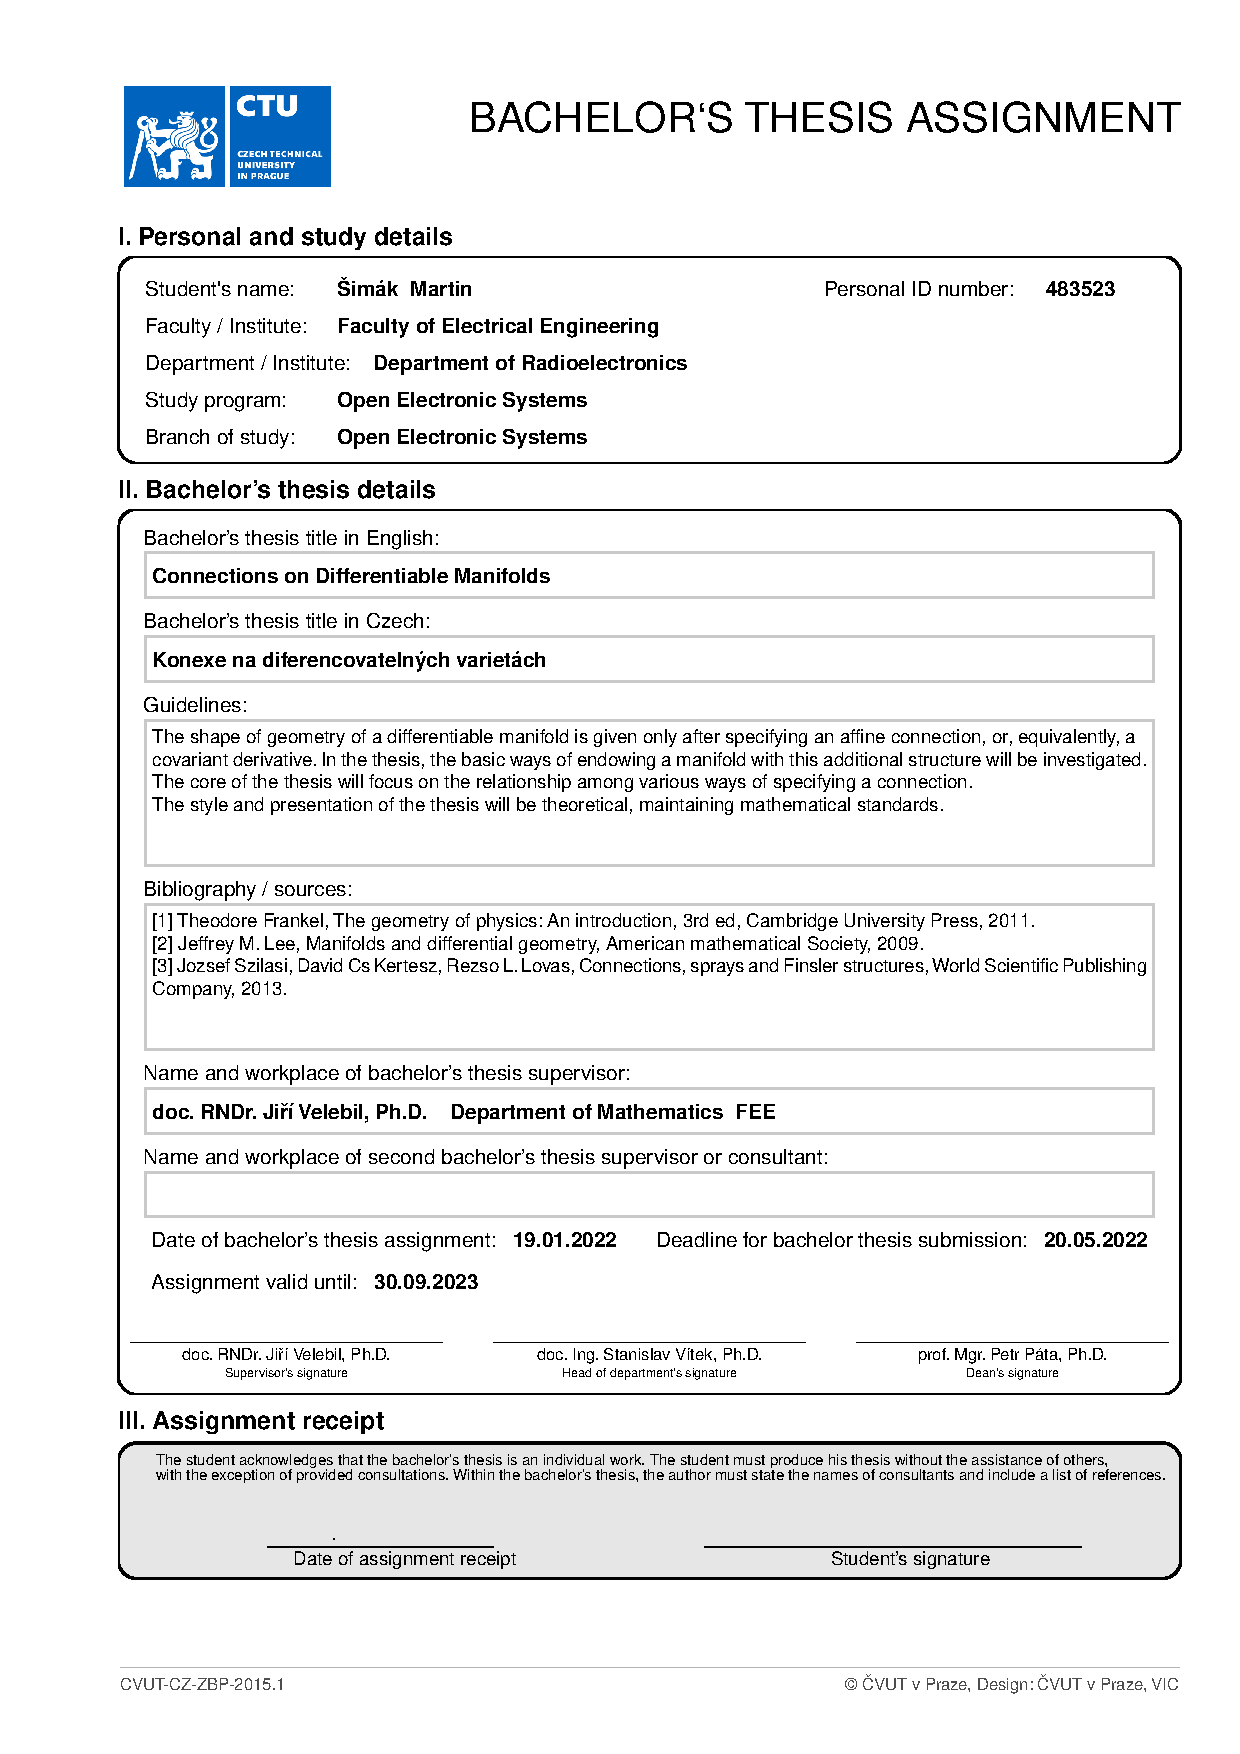
\includepdf[pages=-]{src/assignment.pdf}

% Start counting pages in roman numerals
\pagenumbering{roman}

% %========== Declaration ==========
% \clearpage
\vspace*{\fill}
\noindent\textbf{Declaration}\\[0.25cm]
I declare that I completed the presented thesis independently and that all used sources are quoted in accordance with the Methodological instructions that cover the ethical principles for writing an academic thesis.\\
\hrule\vspace*{1cm}
\begin{otherlanguage}{czech}
    \noindent\textbf{Prohlášení}\\[0.25cm]
    Prohlašuji, že jsem předloženou práci vypracoval samostatně a že jsem uvedl veškeré použité informační zdroje v souladu s Metodickým pokynem o dodržování etických principů při přípravě vysokoškolských závěrečných prací.\\
    \begin{center}
        \begin{minipage}{0.45\textwidth}
            \begin{flushleft}
                V Praze \hdashrule{3cm}{0.5pt}{2pt}
            \end{flushleft}
        \end{minipage}
        ~
        \begin{minipage}{0.45\textwidth}
            \begin{flushright}
                \noindent\begin{tabular}{c}
                    \\
                    \hdashrule{4cm}{0.5pt}{2pt}\\
                    Martin Šimák
                \end{tabular}
            \end{flushright}
        \end{minipage}
    \end{center}
\end{otherlanguage}
\clearpage

% %========== Acknowledgements ==========
% \clearpage
\vspace*{\fill}
\noindent\textbf{Acknowledgements}\\[0.25cm]
Above all, I would like to thank my supervisor, doc. Ing. Pavel Hazdra, Ph.D., for his professional help, willingness, and reliable correspondence throughout our collaboration, which took place remotely during my double degree program in cooperation with the National Taiwan University of Science and Technology. I would also like to thank my supervisor, Ding-Bing Lin, who is responsible for the content of this thesis at the partner university, for his initiative and valuable assistance, especially in the design production. Last but not least, I would like to thank all my loved ones who supported me from afar throughout my studies, especially my family and friends. Special thanks go to Ester \foreignlanguage{czech}{Jančaříková} for standing by me and helping me through difficult times.\\
\hrule\vspace*{1cm}
\begin{otherlanguage}{czech}
    \noindent\textbf{Poděkování}\\[0.25cm]
    Především bych rád poděkoval svému vedoucímu, doc. Ing. Pavlu Hazdrovi, Ph.D., za jeho odbornou pomoc, vstřícnost, a ochotu v podobě spolehlivé korespondence během spolupráce, která probíhala distančně v rámci mého studia double degree programu ve spolupráci s National Taiwan University of Science and Technology. Dále děkuji svému vedoucímu Ding-Bing Linovi, který odpovídá za náplň této práce na partnerské univerzitě, za jeho iniciativu a cennou pomoc, zejména při výrobě návrhu. V neposlední řadě bych rád poděkoval všem svým blízkým, kteří mě na dálku podporovali během celého studia, zejména své rodině a přátelům. Zvláštní poděkování na závěr potom patří Ester Jančaříkové za to, že stála při mě a byla mi oporou v nelehkých chvílích.
\end{otherlanguage}
\clearpage

% %========== Abstract ==========
% \clearpage
\noindent\textit{Title:}\\
\textbf{Dual Circularly Polarized Waveguide Antenna}\\[0.25cm]
\textit{Author:} Martin Šimák\\[0.25cm]
\textit{Study programme:} Electronics and Communications\\[0.25cm]
\textit{Supervisor:} doc. Ing. Pavel Hazdra, Ph.D., Department of Electromagnetic Field FEE\\[0.25cm]
\textit{Abstract:}\\
This thesis details the design, simulation, fabrication, and measurement of a novel dual circularly polarized antenna operating in the $\frequencyrange$ band. The system comprises a square waveguide polarizer with chamfered corners, a dual-coaxial feed, and a conical horn antenna. The polarizer generates right-hand and left-hand circular polarization by selectively exciting one of the two fundamental modes of the square waveguide. The dual coaxial feed provides the necessary excitation. The conical horn, designed using Antenna Magus and adapted to the polarizer, achieves a target gain of $\qty{15}{dBi}$. CST Studio Suite was used for electromagnetic simulations, while Python with SciPy enabled dynamic optimization for enforcing geometric constraints. The fabricated antenna's measured performance closely aligns with simulations, demonstrating an axial ratio below $\qty{5}{dB}$ across the band and a measured gain of approximately $\qty{18}{dBi}$ at the centre frequency. This work contributes to a compact, manufacturable, dual circularly polarized antenna design with potential applications in satellite communications, radar, and other wireless systems.\\[0.25cm]
\textit{Keywords:} circular polarization, waveguide polarizer, dual-feed, conical horn antenna, hexagonal waveguide, eigenmode analysis, electromagnetic simulation\\[0.5cm]
\begin{otherlanguage}{czech}
    \noindent\textit{Název práce:}\\
    \textbf{Duálně kruhově polarizovaná vlnovodová anténa}\\[0.25cm]
    \textit{Autor:} Martin Šimák\\[0.25cm]
    \textit{Studijní program:} Elektronika a komunikace\\[0.25cm]
    \textit{Vedoucí:} doc. Ing. Pavel Hazdra, Ph.D., Katedra elektromagnetického pole FEL\\[0.25cm]
    \textit{Abstrakt:}\\
    Tato diplomová práce popisuje návrh, simulaci, výrobu a měření duální kruhově polarizované antény pracující v pásmu $\frekvencnipasmo$. Systém se skládá ze čtvercového vlnovodného polarizátoru se zkosenými rohy, dvojitého koaxiálního napájení a kuželové antény. Polarizátor generuje pravotočivou a levotočivou kruhovou polarizaci selektivně buzené jedním ze dvou základních módů čtvercového vlnovodu. Potřebné buzení zajišťuje duální koaxiální napájení. Kuželová anténa navržená pomocí programu Antenna Magus a přizpůsobená polarizátoru dosahuje cílového zisku $\qty{15}{dBi}$. Pro elektromagnetické simulace byla použit software CST Studio Suite, zatímco Python s použitím knihovny SciPy umožnil dynamickou optimalizaci pro vynucení geometrických omezení. Naměřený výkon zhotovené antény se přesně shoduje se simulacemi a vykazuje osový poměr pod $\qty{5}{dBi}$ v celém pásmu a naměřený zisk přibližně $\qty{18}{dBi}$ na střední frekvenci. Tato práce přináší kompaktní, vyrobitelnou konstrukci duální kruhově polarizované antény s potenciálním využitím v satelitní komunikaci, radarové technice a dalších bezdrátových systémech.\\[0.25cm]
    \textit{Klíčová slova:} kruhová polarizace, vlnovodný polarizátor, duální napájení, kuželová anténa, hexagonální vlnovod, analýza vlastních módů, elektromagnetická simulace\\[0.5cm]
\end{otherlanguage}
\clearpage

% Start counting pages in arabic numerals
\pagenumbering{arabic}

%========== Table of contents ==========
\tableofcontents

%========== List of figures ==========
\listoffigures

%========== Introduction ==========
\chapter*{Introduction}
\label{chapter:introduction}
\addcontentsline{toc}{chapter}{\nameref{chapter:introduction}}

\lipsum[1-2]
% Do not write a couple of words on literature survey. Present the difference construction and design choices, compare them both theoretically and by the results presented in gathered papers, but in their respective sections of the design process. Use them a nice foreword for each of the parts, going through existing approaches.

Say a few words about the simulation software of choice:
\begin{itemize}
    \item CST Studio Suite~\parencite{cst},
    \item Antenna Magus~\parencite{antenna-magus},
    \item MATLAB~\parencite{matlab}.
\end{itemize}

% Mentioned used optimization method: \emph{Nelder-Mead method}, also called the \emph{downhill simplex algorithm}.

% Maybe chat about frequency band.

% Throughout the theoretical chapter, I omit using the common \emph{del}, or \emph{nabla}, notation for the vector differential operator $\nabla$ which gives rise to the formally proper differential operators of gradient ($\nabla$), divergence ($\nabla\cdot$), curl ($\nabla\times$), and sometimes even the Laplace operator ($\nabla\cdot\nabla$ or $\nabla^2$). Instead, I will use the standard notations of $\Grad$, $\Div$, $\Curl$, and $\Delta$, respectively. While I am aware of the mnemonic merits it brings when working in coordinates, this does not come to fruition as I do not carry out any computations in this text. On the other hand, there are various reasons to avoid it, such as that it promotes a notational ambiguity with the covariant derivative used in differential geometry, or to distinguish the individual operators at first sight better.
% \nomenclature{$\Grad$}{gradient }%
% \nomenclature{$\Div$}{divergence }%
% \nomenclature{$\Curl$}{curl }%
% \nomenclature{$\Delta$}{Laplace operator }%

\paragraph*{Synopsis.} In \textbf{\cref{chapter:electrodynamics}}, \lipsum[4]

\paragraph*{Methodology.} \lipsum[4]


%========== Chapter 1: Electrodynamics of guided waves ==========
\chapter{Electrodynamics of guided waves}
\label{chapter:electrodynamics}
This chapter establishes the theoretical foundation for the analysis and design of a waveguide-based antenna system. Beginning with Maxwell's equations and general description of electromagnetic fields in various settings relevant to this work, the wave equations governing guided waves are derived, and their solutions are analysed to elucidate the behaviour of electromagnetic fields within waveguides. This analysis provides a framework for understanding the operation of structures designed in the following chapters. While focusing on the essential elements of waveguide theory, this chapter provides a comprehensive treatment of the subject and establishes the notation used throughout this work.

The exposition endeavours to take inspiration and build upon the foundations laid in~\parencite{balanis:advanced-engineering-electromagnetics,griffiths:introduction-to-electrodynamics,zangwill:modern-electrodynamics}, incorporating personal insights and notational preferences to present a cohesive theoretical framework for further chapters.

\section{Fundamentals of electrodynamics}
\label{section:fundamentals-of-electrodynamics}
In this section, the fundamental principles of electromagnetism are presented, starting with Maxwell's equations, which encapsulate the relationships between electric and magnetic fields and their sources. The response of different materials to these fields is then explored through the introduction of \emph{constitutive relations}. Finally, the focus is shifted to the behaviour of electromagnetic fields at material boundaries, providing essential \emph{boundary conditions} for solving electromagnetic problems.

\subsection{Maxwell's equations}
\label{subsection:maxwells-equations}
The differential form of Maxwell's equations, as presented below, constitutes the cornerstone of classical electromagnetism, providing a complete%
    \footnote{For actual completeness, save for some special properties stemming from interactions in matter, the equations must also be supplemented by the Lorentz's force law $\vec F = q(\vec E + \vec v \times \vec B)$.}
framework for analysing electromagnetic phenomena at any point in space and time. These equations summarize the relations between \emph{electric field}~$\vec E$ and \emph{magnetic field}~$\vec B$ and their sources due to charge densities~$\rho$, current densities~$\vec J$, or the changing of the fields themselves. To ensure the validity of these expressions, let us assume that the field vectors are well-behaved functions, exhibiting continuity and possessing continuous derivatives. This assumption holds for most electromagnetic systems, with exceptions arising at interfaces between distinct media where abrupt changes in charge and current densities may occur.

\begin{subequations}
    \label[pluralequation]{subeq:maxwell-general}
    \noindent\centering
    \begin{minipage}{0.45\textwidth}
        \begin{align}
            \label{eq:maxwell-general-div-e}
            \div\vec E &= \frac1{\epsilon_0}\rho_{\mathrm e},
        \\
            \label{eq:maxwell-general-curl-e}
            \curl\vec E &= -\mu_0\vec J_{\mathrm m} - \partial_t\vec B,
        \end{align}
    \end{minipage}
    \hfill
    \begin{minipage}{0.45\textwidth}
        \begin{align}
            \label{eq:maxwell-general-div-b}
            \div\vec B &= \mu_0\rho_{\mathrm m},\vphantom{\frac1{\epsilon_0}}
        \\
            \label{eq:maxwell-general-curl-b}
            \curl\vec B &= \mu_0\vec J_{\mathrm e} + \mu_0\epsilon_0\partial_t\vec E,
        \end{align}
    \end{minipage}
    \nomenclature{$\partial_\xi$}{partial derivative w.r.t. variable $\xi$ }%
    \nomenclature{$\vec E$}{electric field }%
    \nomenclature{$\vec B$}{magnetic field }%
    \nomenclature{$\rho_{\mathrm e}$}{electric charge density }%
    \nomenclature{$\rho_{\mathrm m}$}{magnetic charge density }%
    \nomenclature{$\vec J_{\mathrm e}$}{electric current density }%
    \nomenclature{$\vec J_{\mathrm m}$}{magnetic current density }%
    \bigskip
\end{subequations}

There is one oddity about \cref{subeq:maxwell-general} and that is the inclusion of the magnetic charge density $\rho_{\mathrm m}$ and magnetic current density $\vec J_{\mathrm m}$ which are part of the \enquote{generalized concept}. Although these quantities, in spite of diligent search, were never physically observed, their introduction establishes a pleasing balance in Maxwell's equations while being theoretically sound as well. This concept is further utilized when solving advanced physical problems in applied physics and engineering. This is facilitated by the introduction of equivalent magnetic charge and current which can be used to conveniently express fields as if generated by these fictitious sources, especially in problems where the exact form of the electromagnetic field would otherwise be complicated to elucidate.

Mathematically, \cref{subeq:maxwell-general}, like any differential equations, form a complete problem only when supplemented with suitable boundary conditions in a more traditional sense, such as behaviour of the vector fields \enquote{in infinity}. These are typically \enquote{obvious} from the problem-solving context, e.g., fields vanishing at large distance from localized charge distribution, etc.

\subsection{Electromagnetic properties of matter}
Although Maxwell's equations in their fundamental form \eqref{subeq:maxwell-general} provide a complete description of electromagnetic phenomena, an alternative formulation offers a more convenient approach for analysing materials susceptible to electric and magnetic polarization.

Within such media, the total electric charge density~$\rho_{\mathrm e}$ can be expressed as a sum of the \emph{free charge} density~$\rho_{\mathrm f}$, which constitutes the \emph{actual source} charge,%
    \footnote{It is important to reinforce the idea that the magnetic charge and current are fictitious \enquote{source} quantities. Therefore, they are already, by definition, purely \emph{free} quantities.}
and the \emph{bound charge}~$\rho_{\mathrm b}=-\div\vec P$, produced by an electric polarization~$\vec P$ of the material. Moreover, changing electric fields also induce changing polarization, producing \emph{polarization current}~$\vec J_{\mathrm p}=\partial_t\vec P$ which add to the \emph{free current}~$\vec J_{\mathrm f}$. Similarly to electric polarization, a magnetic polarization~$\vec M$ results in a bound current~$\vec J_{\mathrm b}=\curl\vec M$. These effects, inherently connected to the susceptibility of materials to be polarized, hence influence the total electromagnetic field in their vicinity. This led to the introduction of auxiliary field quantities that account for the presence of such media\\
\begin{subequations}
    \label[pluralequation]{subeq:auxiliary-fields}
    \noindent\centering
    \begin{minipage}{0.45\textwidth}
        \begin{align}
            \label{eq:eq:auxiliary-field-d}
            \vec D &= \epsilon_0(\vec E + \vec P)\vphantom{\frac{1}{\mu_0}},
        \end{align}
    \end{minipage}
    \hfill
    \begin{minipage}{0.45\textwidth}
        \begin{align}
            \label{eq:eq:auxiliary-field-h}
            \vec H &= \frac{1}{\mu_0}\vec H - \vec M.
        \end{align}
    \end{minipage}
    \nomenclature{$\vec D$}{auxiliary electric field }%
    \nomenclature{$\vec H$}{auxiliary magnetic field }%
    \bigskip
\end{subequations}\\

This approach allows for expressing Maxwell's equations in a form that directly relates the electric and magnetic fields to the free charge and free current, which are sources that can be controlled directly. Using the field quantities defined by \cref{subeq:auxiliary-fields}, Maxwell's \cref{subeq:maxwell-general} read\\
\begin{subequations}
    \label[pluralequation]{subeq:maxwell-general-matter}
    \noindent\centering
    \begin{minipage}{0.45\textwidth}
        \begin{align}
            \label{eq:maxwell-general-matter-div-d}
            \div\vec D &= \rho_{\mathrm f},
        \\
            \label{eq:maxwell-general-matter-curl-e}
            \curl\vec E &= -\vec J_{\mathrm m} - \partial_t\vec B,
        \end{align}
    \end{minipage}
    \hfill
    \begin{minipage}{0.45\textwidth}
        \begin{align}
            \label{eq:maxwell-general-matter-div-b}
            \div\vec B &= \rho_{\mathrm{m}},
        \\
            \label{eq:maxwell-general-matter-curl-h}
            \curl\vec H &= \vec J_{\mathrm f} + \partial_t\vec D,
        \end{align}
    \end{minipage}
    \bigskip
\end{subequations}

While \cref{subeq:maxwell-general-matter} effectively express electromagnetic laws within media, their hybrid notation, involving both $\vec E$ and $\vec D$, and both $\vec B$ and $\vec H$, necessitates the use of \emph{constitutive relations}. These relations, which establish correspondence between the respective electric and magnetic field quantities, are material-dependent and reflect the specific response of a medium to electric and magnetic fields. In general, these relationships can be expressed as
\begin{subequations}
    \label[pluralequation]{subeq:constitutive-relations}
    \begin{align}
        \label{eq:constitutive-relation-permittivity}
        \vec D &= \hat\epsilon \ast \vec E,
    \\
        \label{eq:constitutive-relation-permeability}
        \vec B &= \hat\mu \ast \vec H,
    \end{align}
    \nomenclature{$\epsilon$}{permittivity }%
    \nomenclature{$\mu$}{permeability }%
    \index{constitutive relations}
    \index{constitutive parameters}
\end{subequations}
where $\hat\epsilon$ and $\hat\mu$ are the material's \emph{permittivity} and \emph{permeability}, respectively, and the asterisk denotes \emph{convolution}.

\begin{remark}
    In formulations of akin to \cref{subeq:maxwell-general-matter}, with emphasis on the separation of free and bound sources, some authors prefer to further dissect the free current, too. This current is generally conceptualized as the current \enquote{not directly tied to the bound charges} within a material. To name a few commonly recognized, \emph{convection current}, \emph{beam current}, or \emph{conduction current}. It is the conduction current which is, in electrical engineering, especially worth mentioning because it arises from the movement of charges, typically electrons, that can move freely throughout the material. This kinetic energy of charges in conductors is the main cause of losses in waveguides and can be expressed by
    \begin{align}
        \label{eq:constitutive-relation-conductivity}
        \vec J_{\mathrm c} &= \hat\sigma \ast \vec E,
        \nomenclature{$\sigma$}{conductivity }%
    \end{align}
    where $\hat\sigma$ is the material's \emph{conductivity}. \Cref{eq:constitutive-relation-conductivity}, together with \cref{subeq:constitutive-relations}, completes the required set of constitutive relations.
\end{remark}

The \emph{constitutive parameters} $\hat\epsilon$, $\hat\mu$, and $\hat\sigma$, generally represented as complex second-rank tensors, establish the relationship between the applied electromagnetic fields and the material's response. The functional dependencies of these tensors provide a classification scheme for material properties:
\begin{itemize}
    \item \emph{Linearity:} A material is classified as linear if its constitutive parameters are independent of the applied field strength; otherwise, it is considered nonlinear.
    \item \emph{Homogeneity:} If the constitutive parameters are invariant with respect to position within the material, it is deemed homogeneous; conversely, spatial dependence indicates an inhomogeneous medium.
    \item \emph{Isotropy:} Materials exhibiting constitutive parameters independent of the applied field's direction are classified as isotropic. Conversely, direction-dependent parameters signify an anisotropic material, with crystals being a prime example.
    \item \emph{Dispersion:} Materials whose constitutive parameters exhibit frequency dependence are categorized as dispersive. While some materials demonstrate negligible frequency dependence and can be effectively considered nondispersive, all materials encountered in practice exhibit some degree of dispersion.
\end{itemize}

\begin{example}[Constitutive relations in free space]
    In the simplest case of free space, equations~\eqref{eq:constitutive-relation-permittivity},~\eqref{eq:constitutive-relation-permeability},~and~\eqref{eq:constitutive-relation-conductivity} become
    \begin{subequations}
        \begin{align}
            \hat\epsilon &= \epsilon_0 \approx 8.854\times 10^{-12}\ \unit{F.m^{-1}},
        \\
            \hat\mu &= \mu_0 = 4\pi\times 10^{-7}\ \unit{H.m^{-1}},
        \\
            \hat\sigma &= \sigma_0 = 0\ \unit{S.m^{-1}}.
        \end{align}
    \end{subequations}
\end{example}

\subsection{Boundary conditions}
While the differential form of Maxwell's equations is a powerful tool for analysing electromagnetic fields within continuous media, material boundaries introduce discontinuities that require special treatment. These discontinuities in the fields arise at interfaces between media with different electrical properties or at surfaces carrying charge or current densities. To accurately describe the behaviour of the fields across such boundaries, Maxwell's equations in their integral form, which naturally incorporate these discontinuities, are more convenient. This form is obtained by applying integral theorems from vector calculus to \cref{subeq:maxwell-general-matter} which then take on the form of
\begin{subequations}
    \label[pluralequation]{subeq:maxwell-equations-integral}
    \begin{align}
        \label{eq:maxwell-equations-integral-div-d}
        \oint_S \vec D \cdot \d\vec a &= Q_{\mathrm{e}},
    \\
        \label{eq:maxwell-equations-integral-curl-e}
        \oint_{\partial S} \vec E \cdot \d\vec l &= -\int_S \vec J_{\mathrm m} \cdot \d\vec a - \frac{\d}{\d t}\int_S \vec B \cdot \d\vec a,
    \\
        \label{eq:maxwell-equations-integral-div-b}
        \oint_S \vec B \cdot \d\vec a &= Q_{\mathrm{m}},
    \\
        \label{eq:maxwell-equations-integral-curl-h}
        \oint_{\partial S} \vec H \cdot \d\vec l &= \int_S \vec J_{\mathrm e} \cdot \d\vec a + \frac{\d}{\d t}\int_S \vec D \cdot \d\vec a,
    \end{align}
    \nomenclature{$\partial\Omega$}{boundary of set $\Omega$ }%
\end{subequations}
\index{boundary conditions}
where $S$ is any closed surface.

Consider a boundary between two different media. The first medium is characterized by permittivity $\epsilon_1$ and permeability $\mu_1$, while the second medium is characterized by permittivity $\epsilon_2$ and permeability $\mu_2$. At this interface, electric and magnetic surface charge densities, denoted by $q_{\mathrm f}$ and $q_{\mathrm m}$, respectively, may be present. Additionally, electric and magnetic surface current densities, denoted by $j_{\mathrm f}$ and $j_{\mathrm m}$, respectively, may also exist. The general \emph{boundary conditions} for electrodynamics are then obtained by applying \cref{subeq:maxwell-equations-integral} to arbitrary surfaces encompassing a portion of the interface, yielding\\
\begin{subequations}
    \label[pluralequation]{subeq:boundary-conditions}
    \noindent\centering
    \begin{minipage}{0.45\textwidth}
        \begin{align}
            \label{eq:boundary-conditions-d-normal}
            \vec e_n \cdot (\vec D_1 - \vec D_2) &= q_{\mathrm f},
        \\
            \label{eq:boundary-conditions-e-tangential}
            -\vec e_n \times (\vec E_1 - \vec E_2) &= \vec j_{\mathrm m},
        \end{align}
    \end{minipage}
    \hfill
    \begin{minipage}{0.45\textwidth}
        \begin{align}
            \label{eq:boundary-conditions-b-normal}
            \vec e_n \cdot (\vec B_1 - \vec B_2) &= q_{\mathrm m},
        \\
            \label{eq:boundary-conditions-H-tangential}
            \vec e_n \times (\vec H_1 - \vec H_2) &= \vec j_{\mathrm f}.
        \end{align}
    \end{minipage}
    \bigskip
\end{subequations}

\section{Electromagnetic waves}
\label{section:electromagnetic-waves}
Having established the foundations of electromagnetism, the focus is now shifted to one of its most significant consequences: the existence of electromagnetic waves. In this section, the manner in which Maxwell's equations predict the propagation of these waves is explored.  The wave equations for the electric and magnetic fields are derived, revealing their interconnected nature and their ability to sustain each other even in the absence of sources. Subsequently, the simplest and most fundamental solutions to these equations, \emph{monochromatic plane waves}, are investigated. Finally, the confinement and guidance of these plane waves within conducting cavities is examined, laying the groundwork for understanding waveguides and resonant structures.

\subsection{The wave equations}
\label{subsection:the-wave-equations}
Maxwell's equations provide a comprehensive description of electromagnetic phenomena, but their coupled nature can make them challenging to solve directly. To facilitate analysis, particularly in source-free regions, it's often advantageous to decouple the equations and express them in terms of the electric and magnetic fields individually. Inside regions with no \emph{free} charge or \emph{free} current, Maxwell's \cref{subeq:maxwell-general-matter} take on the form of\\
\begin{subequations}
    \label[pluralequation]{subeq:maxwell-sourceless}
    \noindent\centering
    \begin{minipage}{0.45\textwidth}
        \begin{align}
            \label{eq:maxwell-sourceless-div-d}
            \div \vec D &= 0,
        \\
            \label{eq:maxwell-sourceless-curl-e}
            \curl \vec E &= -\partial_t\vec B,
        \end{align}
    \end{minipage}
    \hfill
    \begin{minipage}{0.45\textwidth}
        \begin{align}
            \label{eq:maxwell-sourceless-div-b}
            \div\vec B &= 0,
        \\
            \label{eq:maxwell-sourceless-curl-h}
            \curl\vec H &= \sigma\vec E + \partial_t\vec D.
        \end{align}
    \end{minipage}\bigskip
\end{subequations}\\
Furthermore, if the medium is \emph{linear} and \emph{homogeneous}, \cref{eq:maxwell-sourceless-curl-h} can be fully expressed in terms of $\vec E$. With this simplification, applying the curl to \cref{eq:maxwell-sourceless-curl-e,eq:maxwell-sourceless-curl-h} yields\\
\begin{subequations}
    \label[pluralequation]{subeq:wave-equations-lossy}
    \noindent\centering
    \begin{minipage}{0.45\textwidth}
        \begin{align}
            \label{eq:wave-equation-e}
            \Delta\vec E &= \mu\sigma\partial_t\vec E + \mu\epsilon\partial^2_t\vec E,
        \end{align}
    \end{minipage}
    \hfill
    \begin{minipage}{0.45\textwidth}
        \begin{align}
            \label{eq:wave-equation-b}
            \Delta\vec B &= \mu\sigma\partial_t\vec B + \mu\epsilon\partial^2_t\vec B.
        \end{align}
    \end{minipage}\bigskip
\end{subequations}

Therefore, electric and magnetic fields in linear homogeneous media both clearly satisfy the wave equation with a linear damping term $\mu\sigma\partial_t$, introduced by conductive losses. Moreover, in regions with $\sigma = 0$, such as free space or ideal insulators, \cref{subeq:wave-equations-lossy} simplify even more to\\
\begin{subequations}
    \label[pluralequation]{subeq:wave-equations-lossless}
    \noindent\centering
    \begin{minipage}{0.45\textwidth}
        \begin{align}
            \label{eq:wave-equation-e-lossless}
            \Delta\vec E &= \mu\epsilon\partial^2_t\vec E,
        \end{align}
    \end{minipage}
    \hfill
    \begin{minipage}{0.45\textwidth}
        \begin{align}
            \label{eq:wave-equations-b-lossless}
            \Delta\vec B &= \mu\epsilon\partial^2_t\vec B,
        \end{align}
    \end{minipage}\bigskip
\end{subequations}\\
taking on the form of classical wave equations which are ubiquitous in physics. This also immediately gives rise to the formula
\begin{align}
    v &= \frac{1}{\sqrt{\epsilon\mu}} = \frac{c}{\sqrt{\epsilon_r\mu_r}}
\end{align}
for the speed of electromagnetic waves in linear homogeneous media.

\begin{remark}
    \label{remark:nonequivalence-of-wave-equations-with-maxwells-equations}
    Compared with the original Maxwell's \cref{subeq:maxwell-general-matter}, these equations form two systems of second-order partial differential equations but are now decoupled and provide us with an additional solving method for given boundary-value problems. However, it is important to note that the wave \cref{eq:wave-equation-e,eq:wave-equation-b} were derived from Maxwell's \cref{subeq:maxwell-sourceless} by differentiation. This impedes their mathematical equivalence. More specifically, as stated in~\parencite{griffiths:introduction-to-electrodynamics}, whereas every solution to Maxwell's equations is also a solution for the wave equations, the converse is not true.
\end{remark}

\subsection{Monochromatic plane waves}
\index{monochromatic plane wave}
The electromagnetic theory presented thus far describes general vector fields that vary in space and time. However, as shown in \cref{subsection:the-wave-equations}, electromagnetic fields in source-free regions exhibit wave behaviour. Nonetheless, these time-varying vector fields remain complex and challenging to analyse in practical systems. Consider the elementary solution to the wave equation
\begin{align}
    \label{eq:monochromatic-plane-wave}
    \hat{\vec\psi}(\vec r,t) &= \hat{\vec\Psi}_0\exp\[\i\(\hat{\vec k} \cdot \vec r-\omega t\)\].
\end{align}
\nomenclature{$\vec k$}{wave vector }%
Here, $\hat{\vec k}$ is the complex \emph{wave vector} indicating the direction of wave propagation, and $\omega$ is the angular frequency of the wave. \Cref{eq:monochromatic-plane-wave} is expressed in terms of a \emph{complex wave function} with a \emph{complex amplitude} $\hat{\vec\Psi}_0 \equiv \vec\Psi_0\e^{\i\delta}$. This quantity encapsulates both the \emph{real amplitude} $\vec\Phi_0$ and the \emph{phase shift} $\delta$, of the physical wave. A sinusoidal wave representing this solution in physical reality can be extracted from \cref{eq:monochromatic-plane-wave} using the \emph{Euler's formula}, yielding
\begin{align}
    \label{eq:sinusoidal-wave}
    \vec{\psi}(\vec r, t) &= \Re\[\hat{\vec\Psi}_0\exp\[\i\(\hat{\vec k} \cdot \vec r-\omega t+\delta\)\]\] = \Re\[\hat{\vec\psi}(\vec r, t)\].
\end{align}

\begin{remark}
    Clearly, if \cref{eq:sinusoidal-wave} satisfies \cref{subeq:wave-equations-lossless} and Maxwell's equations, the same holds true for \cref{eq:monochromatic-plane-wave}, as the imaginary part differs from the real part only by the replacement of sine with cosine.
\end{remark}

\Cref{eq:monochromatic-plane-wave} serves as as an established elementary solution to the general wave equation, and hence also to \cref{subeq:wave-equations-lossless}. Substituting this solution into \cref{subeq:wave-equations-lossy}, it becomes evident that these \enquote{lossy wave equations} also admit plane-wave solutions. Furthermore, this substitution allows for the derivation of a general formula for the complex \emph{wavenumber}
\begin{align}
    \label{eq:wave-number}
    \hat k^2 = \hat{\vec k} \cdot \hat{\vec k} = \mu\epsilon\omega^2 + \i\mu\sigma\omega.
\end{align}
In the context of \cref{eq:monochromatic-plane-wave}, it is evident that the real part of the complex wavenumber $\hat k$ is the \emph{actual} wavenumber as it determines the change of phase with spatial propagation. For this reason, the real part is simply denoted $k$ and is called the \emph{phase constant}. In contrast, the imaginary part of $\hat k$ is responsible for the exponential damping, or attenuation, in conductive media, and hence is called the \emph{attenuation constant}.

Waves described by \cref{eq:monochromatic-plane-wave} are called \emph{monochromatic}, or \emph{time-harmonic}, \emph{plane}
waves. Monochromaticity refers to the fact that the wave oscillates at a single frequency $\omega$ through time, while planarity indicates that the fields are uniform over every plane perpendicular to the direction of propagation. Although less common, plane waves could alternatively be called \emph{space-harmonic},%
    \footnote{Therefore, monochromatic plane waves are something one could call \emph{spacetime-harmonic} or simply \emph{harmonic}.}
as both of these terms signify a sinusoidal dependence on a given variable. In the case of monochromaticity, the variable is time, oscillating with an angular frequency $\omega$. Similarly, planarity reflects the waveform repetition in the spatial coordinates, projected into the propagation direction, with a well-defined spatial frequency $k$.

The significance of this particular solution stems from the fact that, in practice, any wave relevant to engineering purposes can be expressed as a linear combination of these monochromatic plane waves, i.e.,
\begin{align}
    \label{eq:fourier-transform}
    \hat{\vec\psi}(\vec r,t) &= \int_{\R^3} \hat{\vec{\Psi}}_0(\vec k)\exp\[\i\(\hat{\vec k} \cdot \vec r-\omega t\)\]\,\d\vec k.
\end{align}
This superposition principle mathematically reflects the Fourier transform over every plane wave corresponding to a given frequency $\omega$. With this formally sound mathematical description, the existence of a unique linear combination for \enquote{any wave relevant to engineering purposes}, as vaguely stated above, can be rigorously established.

Indeed, since any physically realizable signal is square-integrable and has compact support,%
    \footnote{In the field of signal processing, these signal properties are often described as having \emph{finite energy} and \emph{duration}, respectively.}
the existence of its Fourier transform is guaranteed. This implication is granted by recalling that the combination of square-integrability and compact support implies, by the Cauchy-Schwarz inequality, absolute integrability which forms a sufficient condition for the existence of the Fourier transform. Therefore, any such physical signal can be confidently decomposed into a superposition of monochromatic plane waves, as expressed in equation \cref{eq:fourier-transform}. This decomposition into a unique linear combination of plane waves of different frequencies underpins much of the mathematical theory concerning Fourier analysis. For a deeper dive into the mathematical foundations of Fourier integrals,~\parencite{titchmarsh:introduction-to-the-theory-of-fourier-integrals} can be consulted. Furthermore, a formulation of Dirichlet conditions which are more attuned to signal processing applications can be found in~\parencite{oppenheim:signals-and-systems}.

Because the focus of this text is confined to signals that are physically realizable and thus possess these crucial properties, a restriction of our attention to monochromatic plane waves is justified. Therefore, fields taking on the form of
\begin{subequations}
    \label[pluralequation]{subeq:monochromatic-plane-wave-fields}
    \begin{align}
        \label{eq:monochromatic-plane-wave-e}
        \hat{\vec E}(\vec r, t) &= \hat{\vec E}_0 \exp\[\i\(\hat{\vec k} \cdot \vec r-\omega t\)\],
    \\
        \label{eq:monochromatic-plane-wave-b}
        \hat{\vec B}(\vec r, t) &= \hat{\vec B}_0 \exp\[\i\(\hat{\vec k} \cdot \vec r-\omega t\)\]
    \end{align}
\end{subequations}
are considered, where $\hat{\vec E}_0$ and $\hat{\vec B}_0$ are complex amplitudes.

As discussed in \cref{remark:nonequivalence-of-wave-equations-with-maxwells-equations}, satisfying the wave equations does not guarantee solutions to Maxwell's equations. Substituting the solutions of the wave equations into Maxwell's equations is necessary, as it might refine the solutions or yield more information. As an example, consider the plane waves in vacuum.

\begin{example}[Monochromatic plane waves in free space]
    Substituting \cref{eq:monochromatic-plane-wave-e,eq:monochromatic-plane-wave-b} for the electric and magnetic field in the free-space version of \cref{eq:maxwell-sourceless-div-d,eq:maxwell-sourceless-div-b} read
    \begin{align}
        \vec k \cdot \hat{\vec E}_0 = \vec k \cdot \hat{\vec B}_0 = 0,
    \end{align}
    \nomenclature{$\vec e_\xi$}{unit vector in the $\xi$-direction }%
    i.e., the electromagnetic fields are \emph{transverse}. Furthermore, either of \cref{eq:maxwell-sourceless-curl-e,eq:maxwell-sourceless-curl-h} yields
    \begin{align}
        \hat{\vec B}_0 &= \frac1\omega\(\vec k \times \hat{\vec E}_0\) = \frac 1c\(\vec e_k \times \hat{\vec E}_0\).
    \end{align}
    Clearly, in free space, $\vec E$ and $\vec B$ are \emph{mutually perpendicular} and \emph{in phase}, meaning their oscillations reach their peaks and troughs simultaneously.
    
    To further characterize the plane wave, a \emph{polarization vector} is introduced. This unit vector points in the direction of electric field oscillations, i.e.,
    \begin{align}
        \vec e_n \cdot \vec E &= \vec E
    &
        \norm{\vec e_n} &= 1.
    \end{align}
    \nomenclature{$\vec e_n$}{polarization vector }%
    \index{polarization vector}%
    With this definition, the complete solution to Maxwell's equations for a plane wave in free space takes the form of
    \begin{align}
        \vec E(\vec r, t) &= E_0\cos(\vec k \cdot \vec r - \omega t + \delta) \vec e_n,
    \\
        \vec B(\vec r, t) &= \frac 1c E_0\cos(\vec k \cdot \vec r - \omega t + \delta) (\vec k \times \vec e_n).
    \end{align}

    It's important to note that this transversality of the electromagnetic fields is a specific property of plane waves in free space or lossless media. When waves are confined in waveguides or propagate through lossy media, the fields generally have longitudinal components as well. This distinction arises because the boundary conditions imposed by the waveguide or the interactions with the medium can alter the field structure.
\end{example}

\subsection{Polarization}
\label{subsection:polarization}
A brief examination of the general polarization properties of monochromatic plane waves is now undertaken. For the sake of simplicity, consideration is restricted to propagation within a vacuum. Consequently, the Cartesian coordinate system is aligned such that the unit vector $e_z$ coincides with the unit vector $e_{\vec k}$ which defines the direction of propagation. The remaining real unit vectors, $\vec e_x$ and $\vec e_y$, are then defined such that $(\vec e_x, \vec e_y, \vec e_z)$ constitutes a right-handed orthogonal triad of unit vectors. Thus, the ordered set of vectors $(\vec e_x, \vec e_y)$ forms a basis for the complex amplitude of the electric field E, and the electric field can thereby be expressed as
\begin{align}
    \label{eq:polarization-e}
    \hat{\vec E}(\vec r,t) &= \[\hat E_x\vec e_x + \hat E_y\vec e_y\]\exp\[\i\phi(\vec r,t)\],
\end{align}
where
\begin{align}
    \hat E_x &= E_x\exp\(\i\delta_x\),
&
    \hat E_y &= E_y\exp\(\i\delta_y\),
\end{align}
for some real numbers $E_x$, $E_y$, $\delta_x$, and $\delta_y$, and
\begin{align}
    \phi(\vec r,t) &= \hat{\vec k} \cdot \vec r - \omega t.
\end{align}
Expressing the real part of \cref{eq:polarization-e} yields
\begin{align}
    \label{eq:polarization-e-real-part}
    \Re\[\hat{\vec E}\] &= E_x\cos\(\phi + \delta_x\)\vec e_x + E_y\cos\(\phi + \delta_y\)\vec e_y = A_x\vec e_x + A_y\vec e_y.
\end{align}
Equating the components from the second relation in \cref{eq:polarization-e-real-part} and applying goniometric identities, the following relationships are obtained:
\begin{subequations}
    \begin{align}
        \label{eq:polarization-ellipse-a}
        \frac{A_x}{E_x}\sin(\delta_y)-\frac{A_y}{E_y}\sin(\delta_x) &= \sin(\delta_y-\delta_x)\cos(\phi),
    \\
        \label{eq:polarization-ellipse-b}
        \frac{A_x}{E_x}\sin(\delta_y)-\frac{A_y}{E_y}\sin(\delta_x) &= \sin(\delta_y-\delta_x)\cos(\phi).
    \end{align}
\end{subequations}
Subsequent squaring and addition of \cref{eq:polarization-ellipse-a,eq:polarization-ellipse-b} yields
\begin{align}
    \label{eq:polarization-ellipse}
    \(\frac{A_x}{E_x}\)^2 + \(\frac{A_y}{E_y}\)^2 - 2\frac{A_x}{E_x}\frac{A_y}{E_y}\cos\(\delta\) &= \sin^2\(\delta\),
\end{align}
\index{elliptical polarization}
where $\delta \equiv \delta_y-\delta_x$. Clearly, \cref{eq:polarization-ellipse} defines an ellipse in the plane transverse to the propagation direction. Accordingly, it can be stated that the general monochromatic plane wave described in \cref{eq:monochromatic-plane-wave} exhibits \emph{elliptical polarization}. The eccentricity and orientation of the ellipse are related to the phase difference $\delta$ and the amplitude ratio $E_y/E_x$. Inspecting \cref{eq:polarization-ellipse}, two special types of polarization can be identified for specific parameter values.

\paragraph{Linear polarization.\index{linear polarization}} The first situation arises when the polarization ellipse degenerates into a straight line. This condition occurs when the electric field components are either in-phase or out-of-phase by half-wavelength, i.e.,
\begin{align}
    \label{eq:polarization-linear-condition}
    \delta = \delta_y-\delta_x = m\pi, \quad m \in \N_0.
\end{align}
This situation corresponds to \emph{linear polarization} and \cref{eq:polarization-e-real-part} is rendered as
\begin{align}
    \label{eq:polarization-linear-e}
    \Re\[\hat{\vec E}(\vec r,t)\] &= \[E_x\vec e_x \pm E_y\vec e_y\]\cos\(\phi + \delta_x\).
\end{align}

\paragraph{Circular polarization.\index{circular polarization}} The alternative scenario arises when the polarization ellipse simplifies into a circle. This simplification occurs exclusively when the orthogonal electric field components possess equal amplitude and are out-of-phase by one-quarter wavelength, i.e.,
\begin{align}
    \label{eq:polarization-circular-condition}
    E_x = E_y &= \frac{E}{\sqrt 2},
&
    \delta = \delta_y-\delta_x &= (2m+1)\frac{\pi}{2}, \quad m \in \Z.
\end{align}
This condition corresponds to \emph{circular polarization}, as the tip of the polarization vector traces a circle within every fixed transverse plane. To ascertain the direction of circular movement, the plane $z=0$ is considered. By setting $\delta_x = 0$,%
    \footnote{The choice $\delta_x=0$ is inconsequential to the resulting polarization as it depends only on the phase difference $\delta$.}
\cref{eq:polarization-e-real-part} is expressed as
\begin{align}
    \label{eq:polarization-circular-e-r0}
    \Re\[\hat{\vec E}_\pm(\vec 0,t)\] &= \frac{E}{\sqrt 2}\[\cos(\omega t)\vec e_x \pm \sin(\omega t)\vec e_y\].
\end{align}
This expression demonstrates that, when viewed from the direction defined by $\hat{\vec k}$, the electric field $\hat{\vec E}^+$ represents a circularly polarized wave with the polarization vector rotating anticlockwise, thus defining \emph{left-hand circular polarization} (LHCP). Conversely, the case of $\hat{\vec E}^-$ represents a circularly polarized wave with the polarization vector rotating clockwise, defining \emph{right-hand circular polarization} (RHCP).

The exposition given so far is aligned with Augustin-Jean Fresnel's general definition of elliptical polarization, as presented in his memoir to the French Academy of Sciences on 9 December 1822, wherein the concepts of the three types of polarization--general elliptical polarization, and its specific forms, linear and circular polarization--were coined. The following remark, however, provides an alternative, and often advantageous, approach.

\begin{remark}[Complex basis for circular polarization]
    For the electric field decomposition basis, the following complex conjugate vectors, rather than the Cartesian vectors $\vec e_x$ and $\vec e_y$, are now considered:
    \begin{align}
        \label{eq:polarization-circular-complex-vectors}
        \vec e_+ &= \frac{1}{\sqrt 2}\(\vec e_x + \i\vec e_y\),
    &
        \vec e_- &= \frac{1}{\sqrt 2}\(\vec e_x - \i\vec e_y\).
    \end{align}
    These vectors maintain orthonormality. Using this basis, it is evident that the real part of the thus formed complex electric field
    \begin{align}
        \hat{\vec E}_\pm(\vec r,t) &= E\vec e_\pm\exp\[\i\(\hat{\vec k}\cdot\vec r - \omega t\)\] = \frac{E}{\sqrt 2}\[\vec e_x \pm \i\vec e_y\]\exp\[\i\(\hat{\vec k}\cdot\vec r - \omega t\)\],
    \end{align}
    evaluated at $\vec r = 0$, is equivalent to \cref{eq:polarization-circular-e-r0}. Because the ordered set of vectors defined by \cref{eq:polarization-circular-complex-vectors} constitutes a valid basis for the transverse plane, analogous to the $(\vec e_x,\vec e_y)$ basis, the expression
    \begin{align}
        \hat{\vec E} &= \[E_+\vec e_+ + E_-\vec e_-\]\exp\[\i\phi\]
    \end{align}
    is an equivalent representation to \cref{eq:polarization-e}. Consequently, any monochromatic plane wave can be decomposed into RHCP and LHCP components, in a manner analogous to its decomposition into orthogonal linearly polarized components.
\end{remark}

\subsection{Guided waves}
The behaviour of electromagnetic waves within a waveguide is now explored. To provide a clear framework for analysis, it is assumed that the waveguide walls are perfect electric conductors (PEC), implying the absence of surface sources. This idealization leads to specific boundary conditions\\
\begin{subequations}
    \label[pluralequation]{subeq:guided-waves-boundary-conditions}
    \noindent\centering
    \begin{minipage}{0.45\textwidth}
        \begin{align}
            \label{eq:guided-waves-boundary-condition-e}
            \vec e_n \times \vec E &= 0,
        \end{align}
    \end{minipage}
    \hfill
    \begin{minipage}{0.45\textwidth}
        \begin{align}
            \label{eq:guided-waves-boundary-condition-b}
            \vec e_n \cdot \vec B &= 0.
        \end{align}
    \end{minipage}\bigskip
\end{subequations}\\
It is important to recognize that free charges and currents will be induced on the surface precisely to enforce these constraints.

Furthermore, the focus is placed on monochromatic plane waves propagating along the waveguide. This implies that the electric and magnetic fields have a harmonic time dependence with a single angular frequency $\omega$. The $\hat{\phantom{x}}$ notation is dispensed with as $\hat k$ is real for the cases of interest. The general form of the fields is then given by \cref{subeq:monochromatic-plane-wave-fields} where the $z$-axis is aligned with the waveguide's longitudinal direction. The complex amplitudes of the fields,\\
\begin{subequations}
    \label[pluralequation]{subeq:complex-amplitudes}
    \noindent\centering
    \begin{minipage}{0.45\textwidth}
        \begin{align}
            \label[pluralequation]{subeq:complex-amplitude-e}
            \hat{\vec E}_0 &= E_x\vec e_x + E_y\vec e_y + E_z\vec e_z,
        \end{align}
    \end{minipage}
    \hfill
    \begin{minipage}{0.45\textwidth}
        \begin{align}
            \label[pluralequation]{subeq:complex-amplitude-b}
            \hat{\vec B}_0 &= B_x\vec e_x + B_y\vec e_y + B_z\vec e_z,
        \end{align}
    \end{minipage}\bigskip
\end{subequations}\\
are functions of the transverse coordinates, $x$ and $y$, reflecting the spatial variations of the fields within the waveguide cross-section.

To further simplify the analysis, the waveguide is considered to be source-free, meaning that there are no free charges or currents \emph{impressed} within the waveguide itself. This allows the utilization of the simplified form of Maxwell's equations \eqref{subeq:maxwell-sourceless}. Due to the assumed linearity of the medium within the waveguide, these equations are expressed in terms of $E$ and $B$.

With these assumptions in place, the wave behaviour within the waveguide can be analysed. From \cref{eq:maxwell-sourceless-curl-e,eq:maxwell-sourceless-curl-h}, adapted for a linear medium, a set of coupled differential equations relating the transverse components of the electric and magnetic fields is obtained. These equations can be solved to express the transverse field components in terms of the longitudinal components, taking the form of\\
\begin{subequations}
    \label[pluralequation]{subeq:guided-wave-transverse-fields}
    \noindent\centering
    \begin{minipage}{0.45\textwidth}
        \begin{align}
            \label{eq:guided-wave-ex}
            E_x &= \zeta\(k\partial_xE_z+\omega\partial_yB_z\)\vphantom{\frac{\omega}{c^2}},
        \\
            \label{eq:guided-wave-ey}
            E_y &= \zeta\(k\partial_yE_z-\omega\partial_xB_z\)\vphantom{\frac{\omega}{c^2}},
        \end{align}
    \end{minipage}
    \hfill
    \begin{minipage}{0.45\textwidth}
        \begin{align}
            \label{eq:guided-wave-bx}
            B_x &= \zeta\(k\partial_xB_z-\frac{\omega}{c^2}\partial_yE_z\),
        \\
            \label{eq:guided-wave-by}
            B_y &= \zeta\(k\partial_yB_z+\frac{\omega}{c^2}\partial_xE_z\),
        \end{align}
    \end{minipage}\bigskip
\end{subequations}\\
where $\zeta = \i/((\omega/c)^2-k^2)$. Finally, substituting \cref{subeq:guided-wave-transverse-fields} into \cref{eq:maxwell-sourceless-div-d,eq:maxwell-sourceless-div-b} leads to uncoupled equations
\begin{subequations}
    \label[pluralequation]{subeq:guided-wave-longitudinal-fields}
    \begin{align}
        \label{eq:guided-wave-ez}
        \[\partial^2_x+\partial^2_y+\(\frac{\omega}{c}\)^2-k^2\]E_z &= 0,
    \\
        \label{eq:guided-wave-bz}
        \[\partial^2_x+\partial^2_y+\(\frac{\omega}{c}\)^2-k^2\]B_z &= 0.
    \end{align}
\end{subequations}
\index{Helmholtz equations}
These equations, often referred to as the \emph{Helmholtz equations}, govern the longitudinal field components and play a crucial role in determining the allowed modes of propagation within the waveguide. These modes are categorized based on the presence or absence of longitudinal components in the electric and magnetic fields. \emph{Transverse electric} (TE) waves have $E_z=0$, while \emph{transverse magnetic} (TM) waves have $B_z=0$. The simplest waves, with both $E_z=B_z=0$ are called \emph{transverse electromagnetic} (TEM) waves, but these cannot exist within a hollow waveguide due to boundary conditions.

\begin{remark}[Non-existence of TEM waves in hollow waveguides]
    \label{remark:nonexistence-of-tem-waves-in-hollow-waveguides}
    To further illustrate this point, consider the case of a waveguide with perfectly conducting walls.
    
    Beginning with the scenario where the longitudinal component of the electric field, $E_z$, is zero, it follows from \cref{eq:maxwell-sourceless-div-d} that the divergence of the electric field in the transverse plane must also be zero. Similarly, when the longitudinal component of the magnetic field, $B_z$, is zero, \cref{eq:maxwell-sourceless-curl-e} dictates that the curl of the electric field in the transverse plane must vanish.
    
    Combining these results, the complex amplitude of the electric field, $\hat{\vec E}_0$, can be expressed as the gradient of a scalar potential $\varphi$ that satisfies the Laplace's equation $\Delta\varphi = 0$. However, the boundary condition on the electric field, as expressed in \cref{eq:guided-waves-boundary-condition-e}, enforces an equipotential at the conductor surface. Since Laplace's equation admits no local extrema, the potential must be constant throughout the waveguide, leading to a zero electric field.
\end{remark}

\begin{remark}[Modal decomposition of guided waves]
    \label{remark:modal-decomposition-of-guided-waves}
    The equations for $E_z$ and $B_z$, \cref{subeq:guided-wave-longitudinal-fields}, are instances of the \emph{Helmholtz equation} with Dirichlet and Neumann boundary conditions, respectively. This mathematical structure the eigenvalue problem for the Laplace operator arising in various physical contexts.
    
    For instance, the same equation and boundary conditions govern the vertical displacements of a vibrating drumhead. In this analogy, TM modes correspond to a drumhead with fixed boundaries, while TE modes correspond to a drumhead with free boundaries. The TM case is also isomorphic to the Schr\"odinger problem for the wave functions and energy eigenvalues of a free particle in a two-dimensional box with hard walls. Seeking inspiration in these analogous problems provides useful intuition when thinking about the modal eigenfunctions and eigenvalues of a waveguide. Some key mathematical results stemming from these analogies include:
    \begin{enumerate}[label=(\alph*)]
        \item There are an infinite number of TE- and TM-mode eigenfunctions.
        \item The eigenvalues are all real and positive.
        \item The eigenfunctions can always be chosen real.
        \item The eigenfunctions form a complete set of functions.
        \item Eigenfunctions belonging to different eigenvalues are orthogonal, i.e.,
        \begin{align}
            \label{eq:mode-orthogonality}
            \int_S \[\hat{\vec E}_{0,\alpha} \times \hat{\vec B}_{0,\beta}^\ast\]\,\d S = C\delta_{\alpha\beta},
        \end{align}
        where $S$ is an arbitrary waveguide cross-section and $\delta_{\alpha\beta}$ is the Kronecker's delta distribution.
    \end{enumerate}


    Perhaps the most significant result in terms of applied electrodynamics is the completeness of the eigenfunctions, which implies that any field within a waveguide can be composed of its modes. Specifically, if $\alpha$ denotes a distinct mode%
        \footnote{For example, in the case of a rectangular waveguide, a mode is given by the combination of two integers, $m$ and $n$.}
    then any wave travelling in the positive direction (denoted by the $+$ superscript) can be decomposed as
    \begin{align}
        \hat{\vec E}^+ &= \sum_\alpha C_\alpha^+\[\hat{\vec E}_{0,\alpha} + \vec e_zE_{z,\alpha}\]\exp\(-\i k_{\alpha}z\),
    \\
        \hat{\vec B}^+ &= \sum_\alpha C_\alpha^+\[\hat{\vec B}_{0,\alpha} + \vec e_zB_{z,\alpha}\]\exp\(-\i k_{\alpha}z\).
    \end{align}
    \index{modal decomposition}
    Similarly, for the negative direction (denoted by the $-$ superscript), the decomposition is given by
    \begin{align}
        \hat{\vec E}^- &= \sum_\alpha C_\alpha^-\[\hat{\vec E}_{0,\alpha} - \vec e_zE_{z,\alpha}\]\exp\(\i k_{\alpha}z\),
    \\
        \hat{\vec B}^- &= \sum_\alpha C_\alpha^-\[-\hat{\vec B}_{0,\alpha} + \vec e_zB_{z,\alpha}\]\exp\(\i k_{\alpha}z\).
    \end{align}
    Furthermore, thanks to the mutual orthogonality of modes, the modal decomposition is uniquely given by the orthogonal projection
    \begin{align}
        C_{\alpha}^\pm &= \frac 12 \frac{\displaystyle\int_S \[\hat{\vec E}_{0,\alpha}^\ast \cdot \hat{\vec E} \pm \(\frac{\omega}{k_\alpha}\)^2 \hat{\vec B}_{0,\alpha}^\ast \cdot \hat{\vec B}\]\,\d S}{\displaystyle\int_S \hat{\vec E}_{0,\alpha}^\ast \cdot \hat{\vec E}_{0,\alpha}\,\d S}\exp\(\pm\i k_\alpha z\),
    \end{align}
    where $S$ is an arbitrary cross-section of the waveguide.
    
    These two results combined lead to a powerful conclusion: the tangential fields within an arbitrary cross-section of the waveguide fully determine the field everywhere within the waveguide. This means that if the tangential components of the electric and magnetic fields are known on a single transverse plane, the entire field distribution within the waveguide can be uniquely determined, both in the transverse plane and along the direction of propagation.
\end{remark}

\begin{example}[TE waves in a rectangular waveguide]
    \label{example:te-waves-in-a-rectangular-waveguide}
    This example delves into the specific case of TE waves within a rectangular waveguide. A waveguide with height $a$ in the $x$-direction and width $b$ in the $y$-direction is considered, the $z$-axis again being aligned with the waveguide's longitudinal direction.  The objective is to derive an expression for the longitudinal component of the magnetic field, $B_z$, using the method of separation of variables. This method involves assuming that, for every $x$ and $y$, $B_z(x,y)$ can be expressed as the product of two independent functions, $X(x)$ and $Y(y)$.

    Substituting this product into \cref{eq:guided-wave-bz} yields a differential equation that can be rearranged by dividing through by $B_z$. This rearranged equation reveals that the $x$-dependent and $y$-dependent terms must be constant, leading to two ordinary differential equations,\\
    \begin{subequations}
        \label[pluralequation]{subeq:rectangular-waveguide-te-odes}
        \noindent\centering
        \begin{minipage}{0.45\textwidth}
            \begin{align}
                \label{eq:rectangular-waveguide-te-ode-x}
                \frac1X X'' &= -k_x^2,
            \end{align}
        \end{minipage}
        \hfill
        \begin{minipage}{0.45\textwidth}
            \begin{align}
                \label{eq:rectangular-waveguide-te-ode-y}
                \frac1Y Y'' &= -k_y^2.
            \end{align}
        \end{minipage}\bigskip
    \end{subequations}\\
    Additionally, a relationship between the separation constants, $k_x$ and $k_y$, and the wave number, $k$, is established as
    \begin{align}
        \label{eq:rectangular-waveguide-te-k}
        -k_x^2-k_y^2+\(\frac\omega c\)^2 - k^2 &= 0.
    \end{align}

    \Cref{eq:rectangular-waveguide-te-ode-x} is a simple second-order ordinary differential equation, with a general solution of the form
    \begin{align}
        X(x) &= A\sin(k_xx)+B\cos(k_xx).
    \end{align}
    To determine the particular solution, boundary conditions must be applied. The boundary condition~\eqref{eq:guided-waves-boundary-condition-b} enforces the vanishing of $B_x$ at $x=0$ and $x=a$. According to \cref{eq:guided-wave-bx}, this translates to enforcing the vanishing of $\partial_xB_z = X'$ at those points. This implies $A=0$ and the separation constant $k_x$ must satisfy the condition
    \begin{align}
        \label{eq:rectangular-waveguide-te-kx}
        k_x &= \frac{m\pi}{a},\quad m \in \N_0.
    \end{align}
    Similarly, for the function $Y(y)$, the boundary condition leads to the condition
    \begin{align}
        \label{eq:rectangular-waveguide-te-ky}
        k_y &= \frac{n\pi}{b},\quad n \in \N_0.
    \end{align}
    Combining these results, the particular solution for $B_z$ takes the form of
    \begin{align}
        \label{eq:rectangular-waveguide-te-bz}
        B_z(x,y) &= B_0\cos\(\frac{m\pi}{a}x\)\cos\(\frac{n\pi}{b}y\),
    \end{align}
    representing the $\TE mn$ wave with the corresponding wavenumber given by \cref{eq:rectangular-waveguide-te-k}. This information is a complete solution to the wave propagation since the remaining field components are given by \cref{subeq:guided-wave-transverse-fields}.

    Examining \cref{eq:rectangular-waveguide-te-k}, it becomes evident that if the frequency falls below a certain \emph{cutoff frequency},
    \begin{align}
        \label{eq:cutoff-frequency}
        f_{mn} \equiv \frac c2\sqrt{\(\frac ma\)^2 + \(\frac nb\)^2},
    \end{align}
    \index{cutoff frequency}
    the wavenumber becomes imaginary. This signifies that the wave cannot propagate and instead decays exponentially within the waveguide. Such solutions are referred to as \emph{evanescent waves}. This cutoff frequency depends on the mode numbers $(m, n)$ and the dimensions of the waveguide $(a, b)$. Modes having the same cutoff frequency are called \emph{degenerate}.
    \index{degenerate modes}

    The wavelength corresponding to wavenumber $k$ in the direction of guided wave propagation is called the \emph{guide wavelength} and is given by
    \begin{align}
        \label{eq:guide-wavelength}
        \lambda_{\mathrm g} \equiv \frac{2\pi}{k} &= \frac{\lambda}{\sqrt{1-\(\dfrac{f_{mn}}{f}\)^2}} = \frac{\lambda}{\sqrt{1-\(\dfrac{\lambda}{\lambda_{mn}}\)^2}}.
    \end{align}
    \index{guide wavelength}
    This guide wavelength is related to the free-space wavelength, $\lambda$, and the cutoff wavelength, $\lambda_{mn}$, for the $\TE mn$ mode.
\end{example}

\paragraph{To do:} Maybe add some talk about modes to finish the theoretical chapter smoothly. Perhaps something about frequency dependence of modes' evanescence or something along the lines of that\dots

\chapter{Polarizer}
\label{chapter:polarizer}
The design process of a waveguide polarizer is detailed in this chapter. An initial survey of existing literature, including relevant conference papers and research articles, is undertaken. Based on this survey, the performance characteristics of various design concepts are compared and contrasted. A solution to the design problem is then proposed, with a rationale provided for the selected approach. Following this selection, an in-depth eigenmode analysis of the chosen structure is performed. This analysis, as will be demonstrated in this chapter, yields crucial insights into the operational principles, allows for the recognition of key performance parameters, and provides the foundation for the definition of the optimization problem. The chosen structure is subsequently implemented and optimized within CST Studio Suite for a specified target frequency band. The inherent trade-offs between key performance parameters are then discussed, with reference to established principles of guided wave propagation in rectangular waveguides. Finally, the simulated performance of the designed component is presented graphically, derived from full-wave simulations.

\section{Principle of operation}
To achieve dual polarization, the inherent characteristics of symmetric waveguides are leveraged. This choice stems from their unique ability to enable independent control over two orthogonal polarization states possessing identical propagation characteristics.  Such independent control is essential for polarization manipulation, allowing for the adjustment of the relative phase and amplitude of these orthogonal modes to achieve the desired polarization states. This capability is directly applied in the design of the dual linear-to-circular polarizer detailed herein. The desired polarization states of RHCP and LHCP were mathematically elaborated on in \cref{subsection:the-wave-equations}.

This crucial characteristic arises from two fundamental properties rooted in the electrodynamics of symmetric waveguides. Firstly, their geometric symmetry (manifesting as mirror or rotational symmetry) permits the existence of two fundamental degenerate modes. A rectangular waveguide, as illustrated in \cref{example:te-waves-in-a-rectangular-waveguide}, exhibits this with its $\TE 10$ and $\TE 01$ modes. Secondly, as detailed in \cref{remark:modal-decomposition-of-guided-waves}, a fundamental principle derived from Maxwell's equations dictates that any two distinct modes within a waveguide are orthogonal. This orthogonality, expressed mathematically in \cref{eq:mode-orthogonality}, ensures that the power flow associated with the interaction of any two distinct modes is zero. In essence, transverse symmetry enables the existence of orthogonally polarized modes, while their inherent orthogonality guarantees their independent propagation without coupling or interference.

The description of circular polarization expressed compactly in \cref{eq:polarization-circular-condition} establishes a clear objective for the design of a waveguide polarizer: the creation of a segment, based on a symmetrical waveguide, that introduces a one-quarter wavelength phase difference between the two orthogonal modes along its length, while maintaining equal magnitudes. In subsequent design stages, this latter criterion is quantified by a singular metric known as the \emph{axial ratio} of the emitted wave, which characterizes the polarization purity based on its far-field properties. Several widely adopted approaches exist for achieving these objectives; these may be referred to as standard methods. Notable examples include the following:
\begin{itemize}
    \item \emph{Dielectric vane polarizers} utilize a dielectric element (a so-called quarter-wave plate) inserted into a segment of a symmetrical waveguide at an angle of $\pm \ang{45}$ relative to the incident electric field. The inserted dielectric introduces a difference in the propagation velocities of the two orthogonal modes along this segment. This differential propagation velocity arises from the interaction of one mode with the vane, which reduces its propagation velocity due to its parallel orientation relative to the vane, while the orthogonal mode remains unaffected due to its perpendicular orientation.

    \item \emph{Septum polarizers} comprise two rectangular ports converging at a stepped septum and extending into a symmetrical waveguide. When the structure is excited through one of these ports, the septum polarizer converts approximately half of the incident energy to the orthogonal polarization, achieving circular polarization through the introduction of a one-quarter wavelength phase shift at the output port. Excitation of the structure through the alternate port results in circular polarization of the opposite handedness.

    \item \emph{Iris polarizers} utilize symmetrical waveguides with non-trivial cross-sections, incorporating ridges, also referred to as corrugations or irises, typically positioned symmetrically on two opposing sides. These polarizers operate on a linearly polarized wave incident diagonally into the waveguide. In this configuration, the ridges present inductive characteristics to one of the waveguide modes and capacitive characteristics to the orthogonal mode. This differential interaction results in a one-quarter wavelength phase delay at the output port.
\end{itemize}

\section{Literature survey}
While the methods established above can be refined and adjusted to achieve favourable results in typical metrics for linear-to-circular polarizers, each also exhibits inherent limitations. Dielectric vane polarizers, while simple to implement, are known to encounter narrow bandwidth issues and suffer from significant power limitations due to inherent dielectric losses. The dielectric losses are encompassed in \cref{eq:wave-number} as any real dielectric exhibits a small but non-zero conductivity $\sigma > 0$. These losses become particularly pronounced at higher frequencies and power levels, restricting their applicability in certain scenarios. In contrast, septum polarizers offer promising capabilities for a wide range of applications, particularly in terms of power handling and the efficient generation of both right-hand and left-hand circular polarizations. As noted by~\parencite{ruiz-cruz-et-al:compact-reconfigurable-waveguide-circular-polarizer} modifications to septum designs, such as the integration of RF MEMS switches, can achieve reconfigurability and control over the handedness of the produced circular polarization elegantly. However, the size and weight of septum structures can pose significant constraints, especially in compact or weight-sensitive applications. Furthermore, as highlighted by~\parencite{wang-et-al:novel-square-rectangle-waveguide-septum-polarizer}, alternative septum geometries, such as tapered slots, while offering potential design variations, do not necessarily demonstrate substantial performance improvements over conventional stepped septum designs. Iris polarizers, while capable of converting linearly polarized input into both circular polarizations and operating at higher power levels, often exhibit challenges related to \enquote{overmoding} within their structures, necessitating precise mode-matching to maintain a satisfactory axial ratio across a broad frequency band. As observed by~\parencite{song-et-al:design-of-wideband-quad-ridge-waveguide-polarizer}, variations in iris design, such as incorporating ridges on four sides instead of two, can be explored. Moreover, as emphasized by~\parencite{virone-et-al:optimum-iris-set-concept-for-waveguide-polarizers}, the design of iris arrays requires extensive analysis of the optimal geometry, often involving complex mathematical techniques, to achieve desired performance characteristics. This complexity is further compounded when considering wider bandwidth operation, as noted by~\parencite{piltyay-et-al:new-tunable-iris-post-square-waveguide-polarizers-for-satelliste-information-systems}, which may necessitate cascading individual sections and careful consideration of different ridge types and transmission matrix approaches. Finally, as demonstrated by~\parencite{deutschmann-arne:broadband-septum-polarizer-with-triangular-common-port}, innovative manufacturing techniques, such as additive manufacturing, combined with alternative waveguide geometries like triangular waveguides, offer potential avenues for further advancement in polarizer design, encompassing design, manufacturing, and measurement aspects.

Departing from these standard methods, various waveguide geometries can be employed for electromagnetic wave manipulation. While standard rectangular and circular waveguides are commonplace, specialized applications such as polarization control often necessitate the use of waveguides with modified cross-sections to introduce a controlled phase difference between orthogonal modes, thereby achieving the desired polarization state. Two prominent examples of such modified waveguides include elliptical waveguides and waveguides with shaped metallic inserts. Elliptical waveguides, as demonstrated in~\parencite{yu-et-al:a-wideband-circularly-polarized-horn-antenna-with-a-tapered-elliptical-waveguide-polarizer} in the context of a wideband circularly polarized horn antenna, leverage their inherent anisotropy to induce the required phase shift. The use of tapered elliptical waveguides, as also explored in~\parencite{yu-et-al:a-wideband-circularly-polarized-horn-antenna-with-a-tapered-elliptical-waveguide-polarizer}, facilitates wideband operation. Waveguides with shaped metallic inserts, on the other hand, introduce field perturbations to achieve the desired polarization transformation. As shown in~\parencite{rud-shpachenko:polarizers-on-sections-of-square-waveguides-with-inner-corner-ridges,bhardwaj-volakis:hexagonal-waveguides-new-class-of-waveguides-for-mmwave-circularly-polarized-horns,bhardwaj-volakis:hexagonal-waveguide-based-circularly-polarized-horn-antennas-for-submmwave-terahertz-band,bhardwaj-volakis:circularly-polarized-horn-antennas-for-terahertz-communications-using-differential-mode-dispersion-in-hexagonal-waveguides}, these inserts can take various forms, including square or triangular blocks inserted into diagonally opposite corners of a square waveguide. This configuration, as validated in~\parencite{rud-shpachenko:polarizers-on-sections-of-square-waveguides-with-inner-corner-ridges} and~\parencite{bhardwaj-volakis:hexagonal-waveguides-new-class-of-waveguides-for-mmwave-circularly-polarized-horns}, introduces a shorter electrical path for one mode, resulting in a phase delay along the polarizer's length. Furthermore, as explored in~\parencite{garcia-marin-masa-campos:bowtie-shaped-radiating-element-for-single-and-dual-circular-polarization}, more optimal cross-sectional shapes, such as a bow-tie configuration, can enhance performance, although often at the expense of increased manufacturing complexity. While the higher frequency regions targeted in most of the explored articles are not the primary focus of this work, the underlying principles of achieving polarization control through modified waveguide cross-sections provide valuable insights and inspiration for the design of the polarizer presented herein.

\paragraph{Selected approach.} This thesis introduces a novel approach to achieving enhanced polarization purity by employing a straightforward and robust cross-sectional geometry. This geometry is realized by inserting simple shapes into two opposing sides of a waveguide's cross-section. Initially, both square and circular waveguides, each suitable for dual linear-to-circular polarization conversion, are examined and compared to determine the more advantageous geometry. For the square waveguide illustrated in \cref{fig:polarizer-square-perspective}, triangular prisms are inserted into two opposing corners, forming a hexagonal waveguide as seen in~\parencite{bhardwaj-volakis:hexagonal-waveguides-new-class-of-waveguides-for-mmwave-circularly-polarized-horns}, while cylindrical segments are used for the circular waveguide in \cref{fig:polarizer-circular-perspective}. This concept is inspired by the established technique of chamfering opposing corners of a circularly polarized patch antenna. The resulting waveguide structures can be considered Babinet-complementary%
    \footnote{This name refers to the notion of complementary structures according to \emph{Babinet's principle}, derivation of which is out of scope for this text. More details can be found, e.g., in~\parencite{born-wolf:principles-of-optics}.}
to this antenna configuration.

\begin{figure}[!ht]
    \centering
    \begin{subfigure}{.45\textwidth}
        \centering
        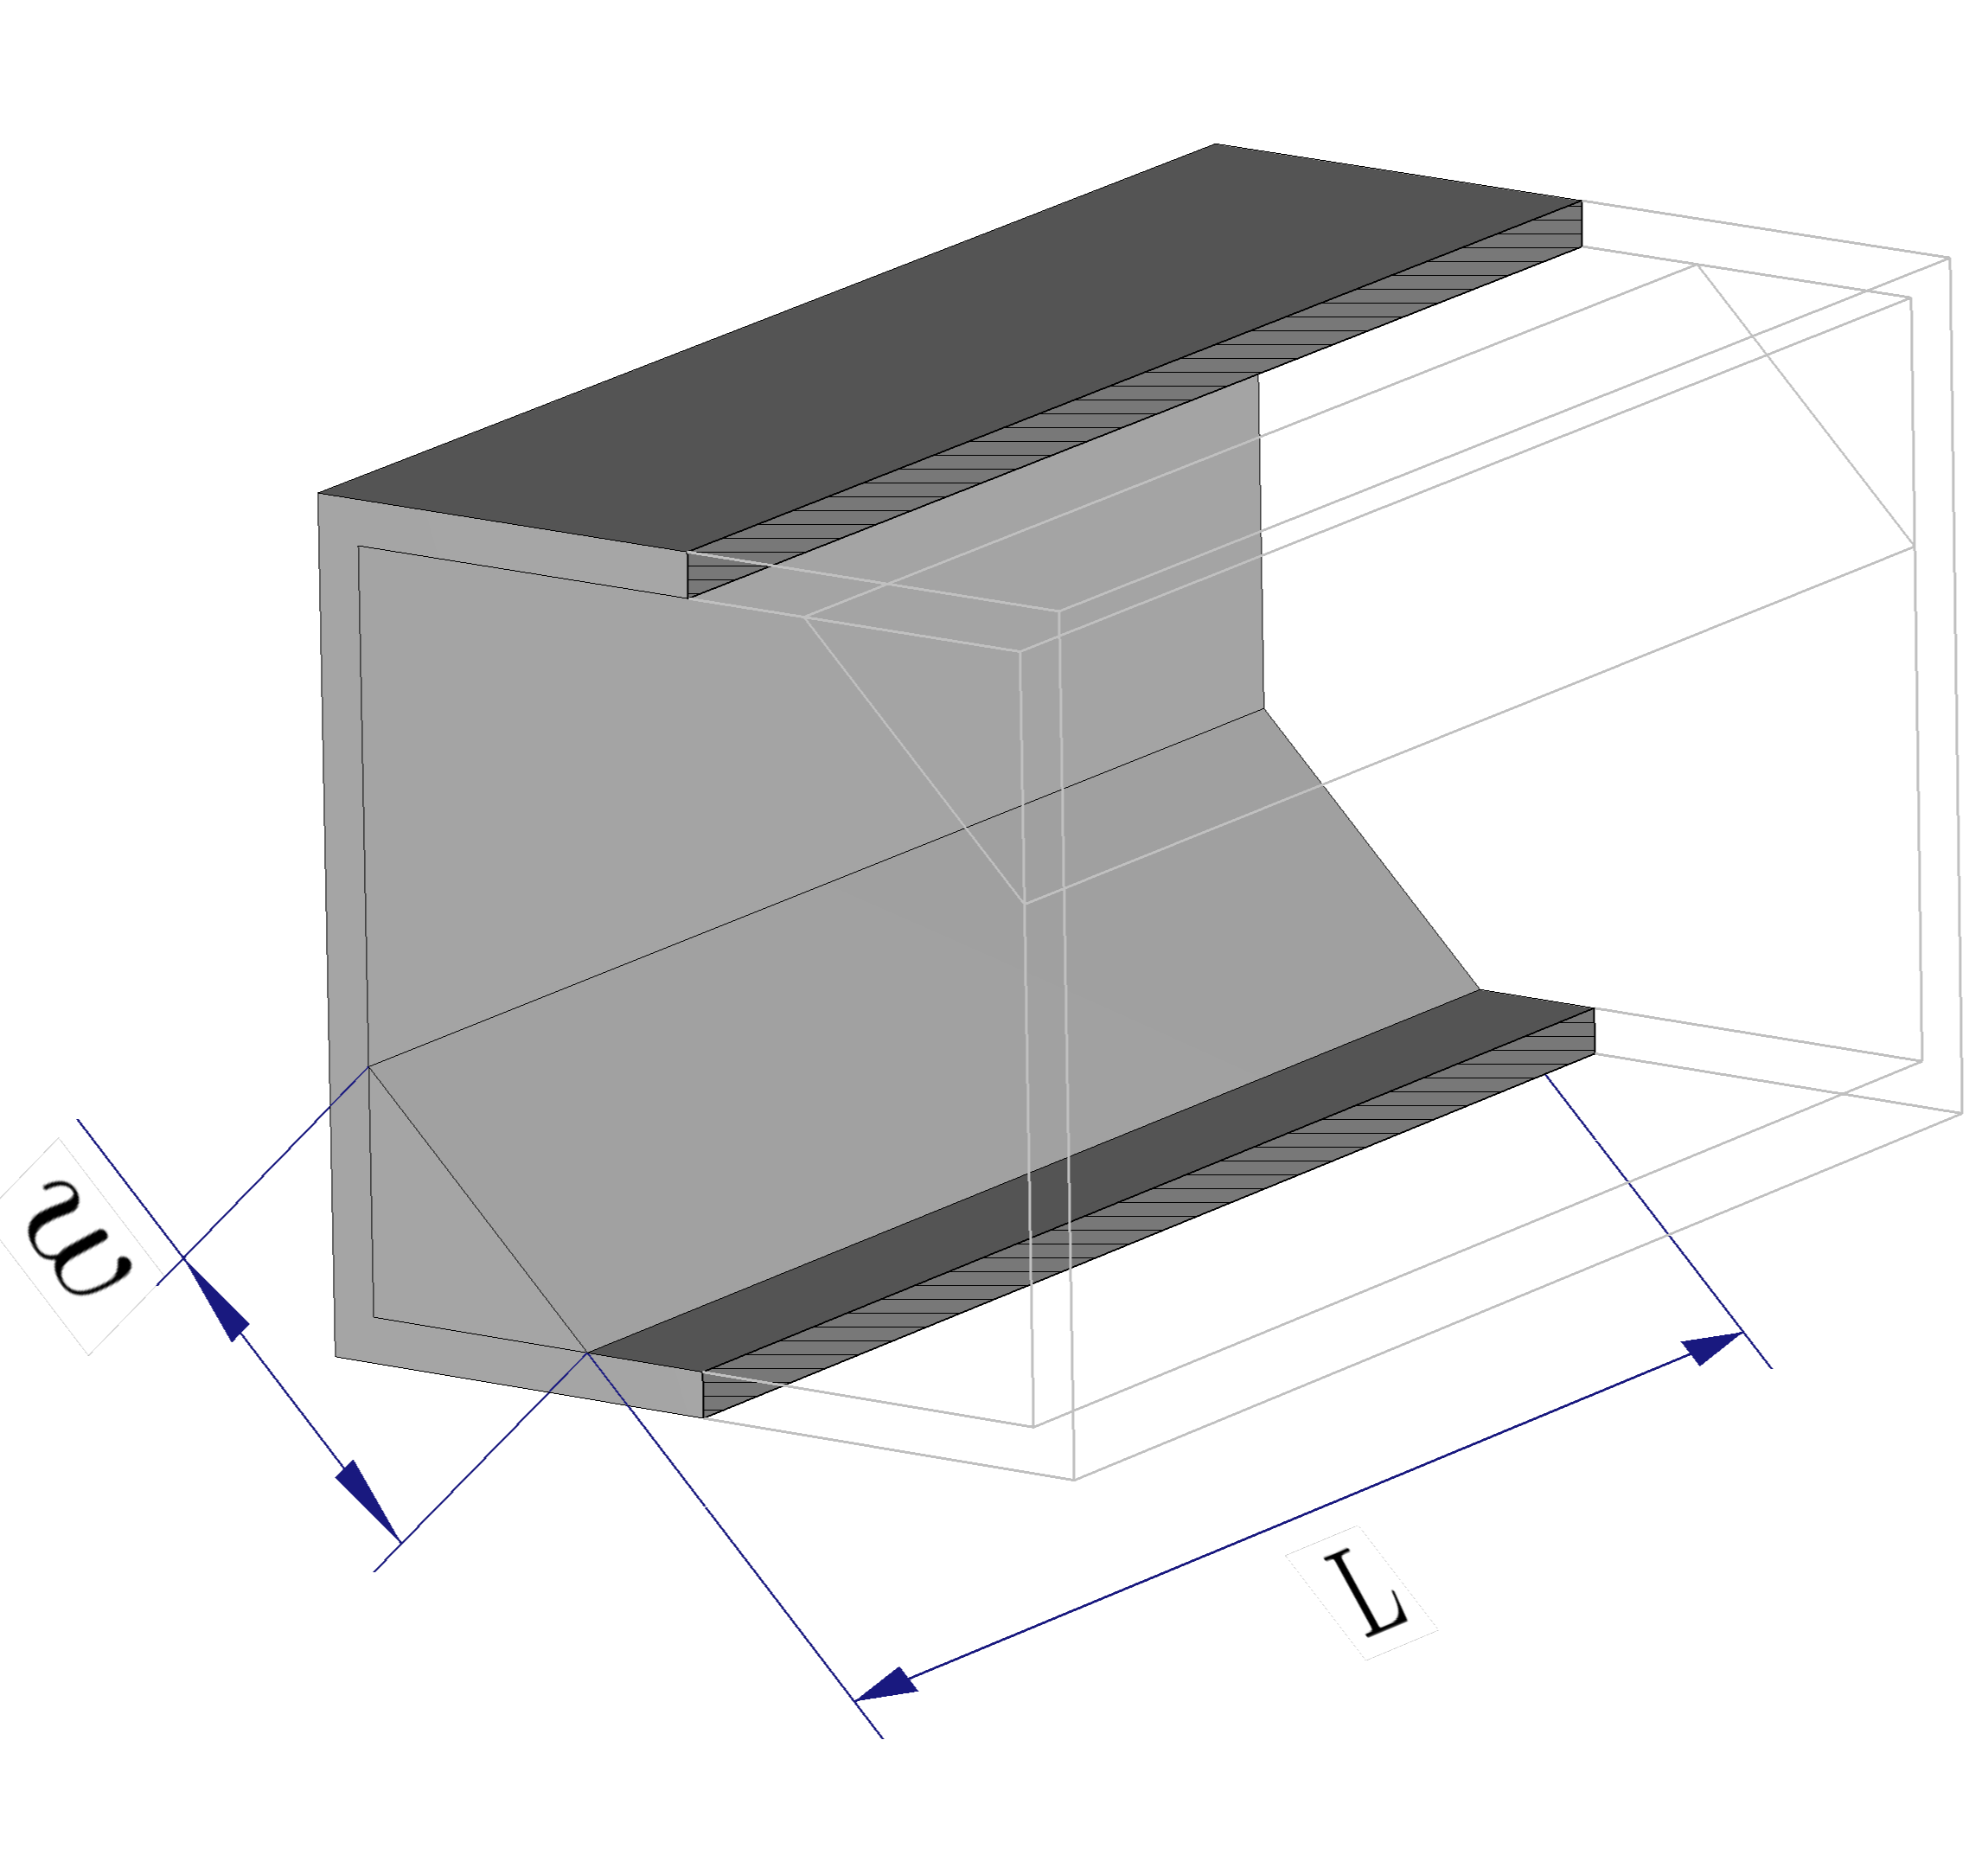
\includegraphics[width=\textwidth]{src/polarizer_square_perspective.png}
        \caption{\label{fig:polarizer-square-perspective}}
    \end{subfigure}
    \hfill
    \begin{subfigure}{.45\textwidth}
        \centering
        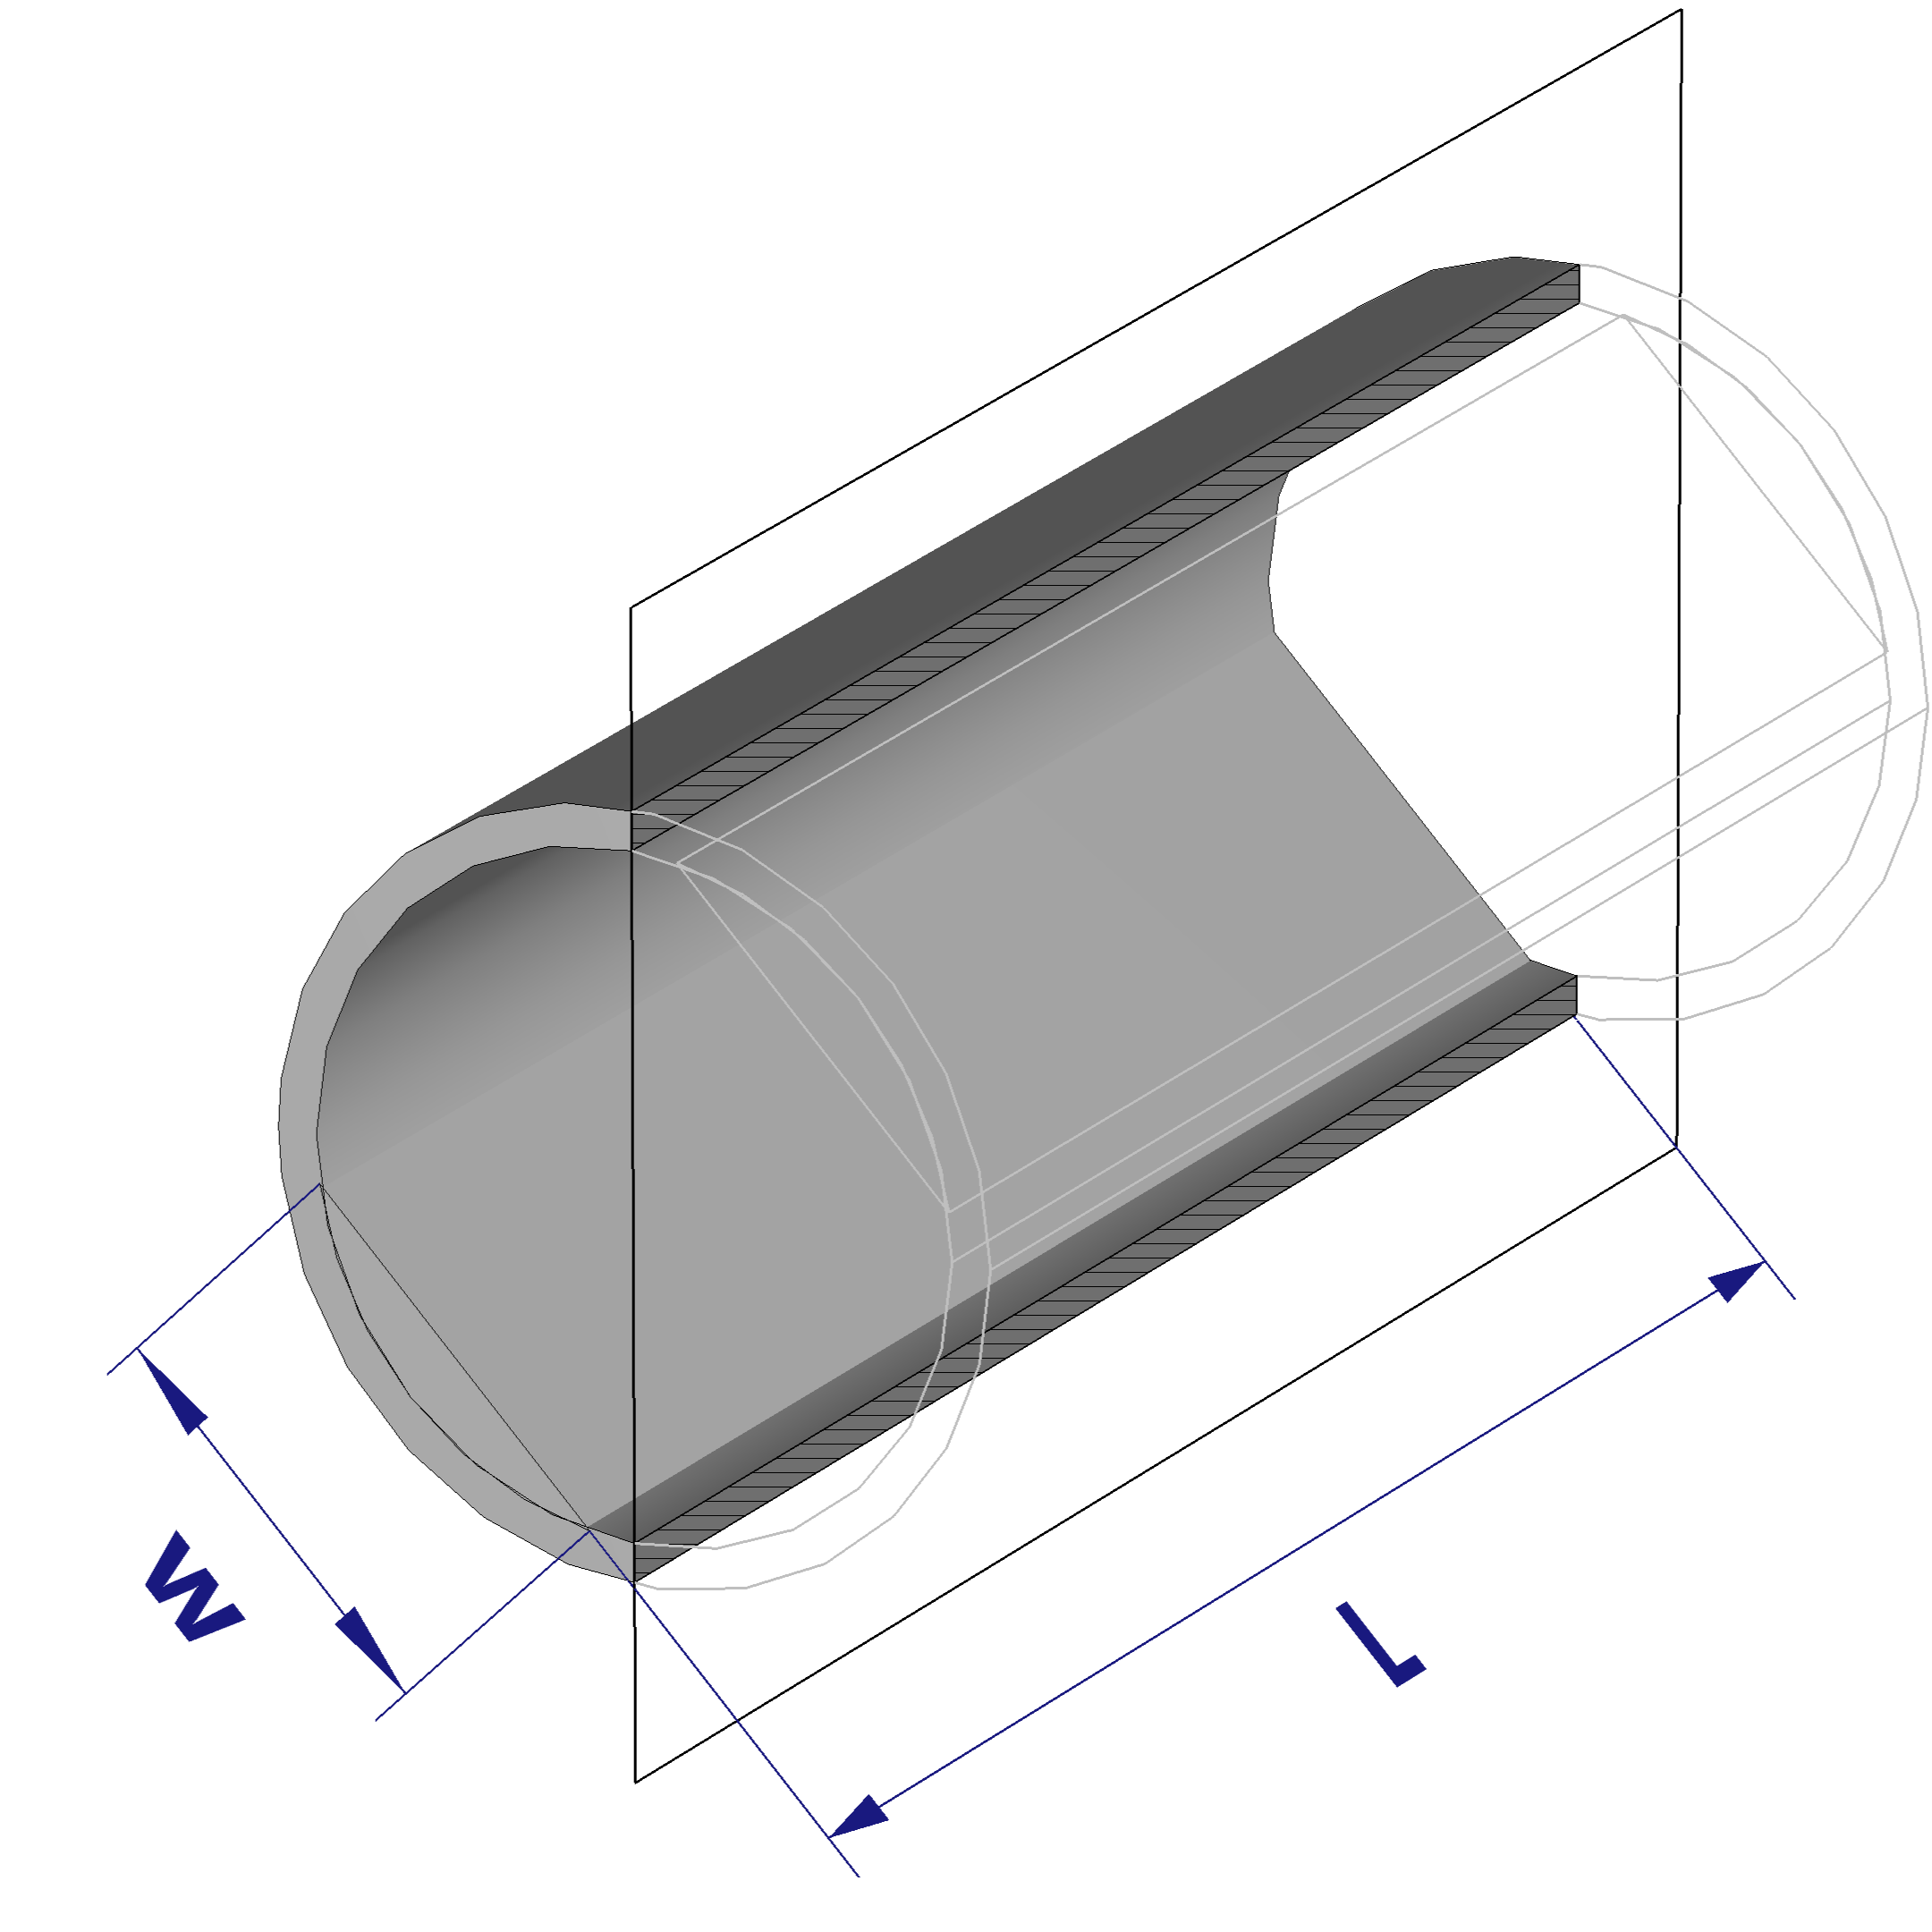
\includegraphics[width=\textwidth]{src/polarizer_circular_perspective.png}
        \caption{\label{fig:polarizer-circular-perspective}}
    \end{subfigure}
    \caption{\label{fig:polarizers}Symmetric polarizers: models}
\end{figure}

This approach was selected primarily for its relative ease of fabrication, particularly at higher frequencies, and its potential for adaptation to various frequency bands. However, due to the resonant, and hence geometry-dependent, nature of the mode dispersion introduced by the metallic inserts, optimal performance is anticipated over a moderately wide bandwidth, rather than an ultrawide one. This bandwidth limitation represents a trade-off for the design's simplicity, robustness, and manufacturability. The use of triangular prisms, in particular, simplifies fabrication compared to more complex curved geometries while still providing effective field manipulation for polarization control.

\section{Eigenmode analysis}
The focus now shifts to the \emph{eigenmode analysis} the two waveguides illustrated in \cref{fig:polarizers}. This powerful technique, based on the theory outlined in \cref{remark:modal-decomposition-of-guided-waves}, facilitates the establishment of figures of merit intrinsic to polarizing structures, enabling performance tracking and aiding in the determination of the more advantageous geometry.

Initially, the fundamental modes of propagation in the symmetric waveguides, \emph{without} the inserted shapes, are considered. In the case of the square waveguide, it is the $\TE 10$ and $\TE 01$ modes illustrated in \cref{fig:square-waveguide-mode1,fig:square-waveguide-mode2}, whereas the two degenerate $\TE 11$ modes%
    \footnote{Note that circular waveguides posses an infinite number of degenerate $\TE 11$ modes due to their rotational symmetry. Here, two are chosen for their perpendicular oscillations which aligns well with the definition of circular polarization in \cref{subsection:polarization}.}
of the circular waveguide are presented in \cref{fig:circular-waveguide-mode1,fig:circular-waveguide-mode2}. For both waveguides individually, these two degenerate modes represent the two waves launched into the polarizer via a section of standard waveguide. Upon encountering the metallic inserts, such incident wave no longer represents the eigenmode of the simple waveguide structure and its energy is coupled into a linear combination of the fundamental eigenmodes of the respective polarizer.

\begin{figure}[!ht]
    \centering
    \begin{subfigure}{.45\textwidth}
        \centering
        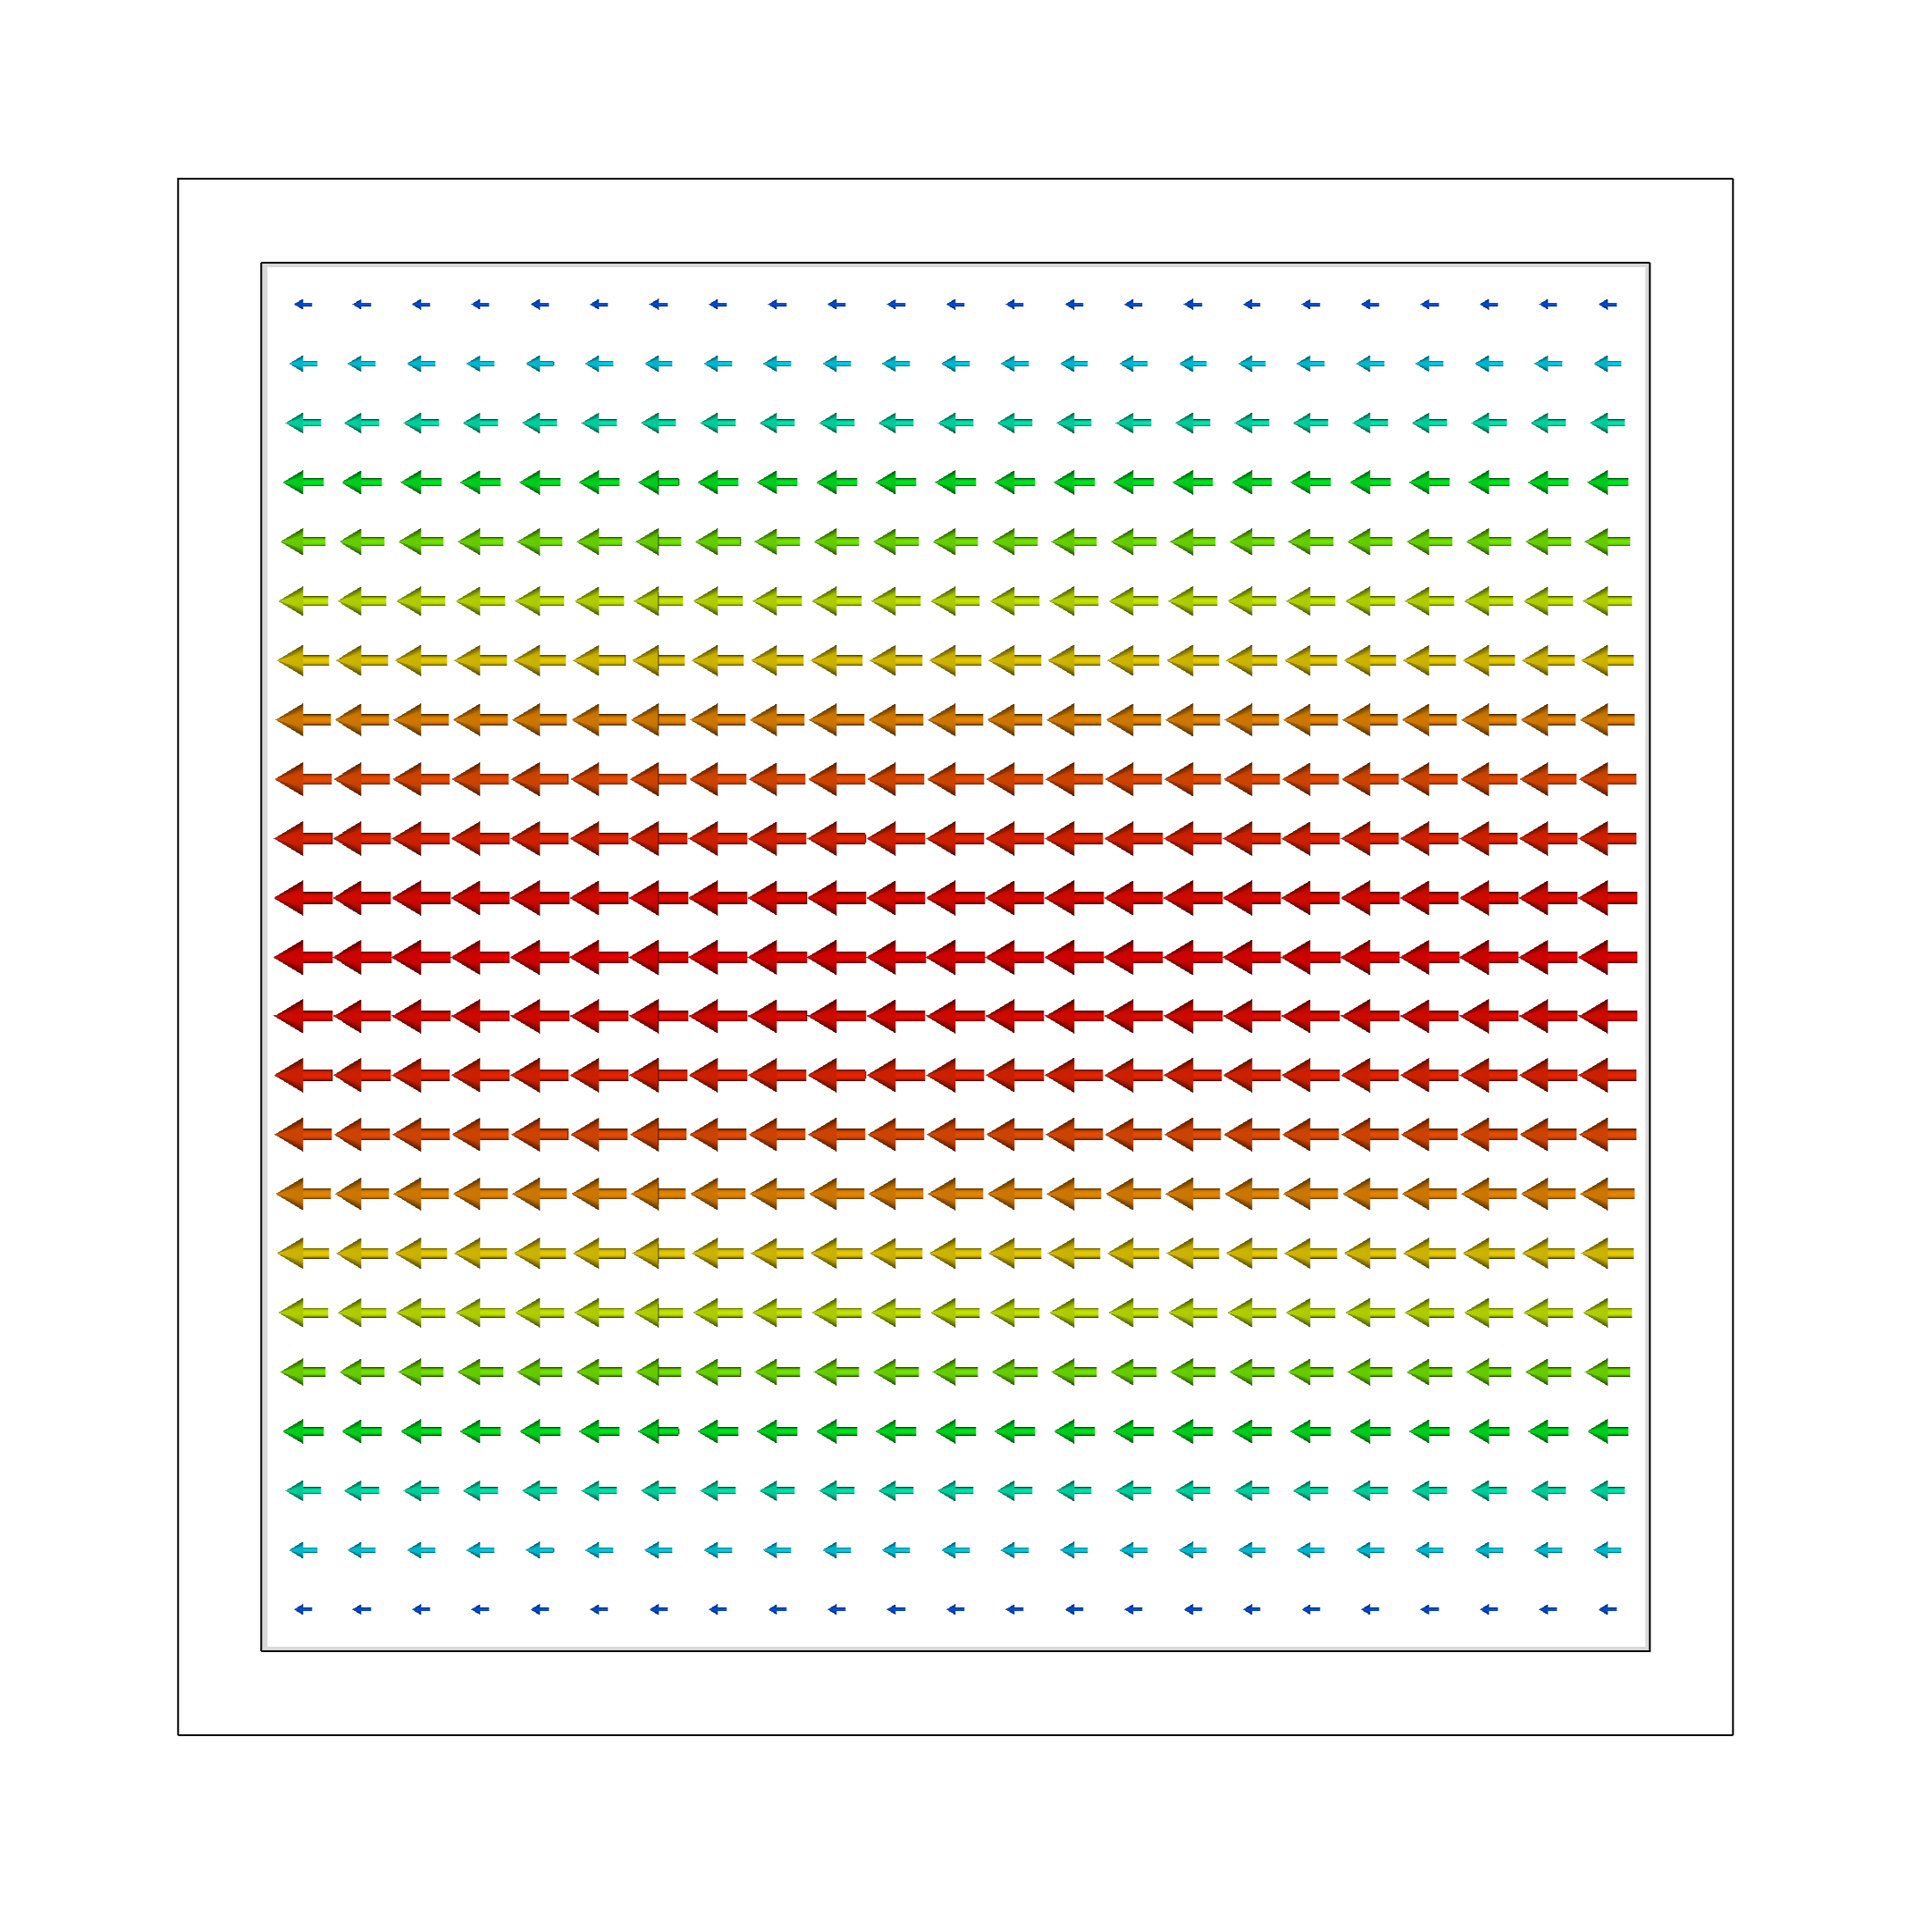
\includegraphics[width=.75\textwidth]{src/waveguide_square_mode1.png}
        \caption{\label{fig:square-waveguide-mode1}}
    \end{subfigure}
    \hspace{0.5cm}
    \begin{subfigure}{.45\textwidth}
        \centering
        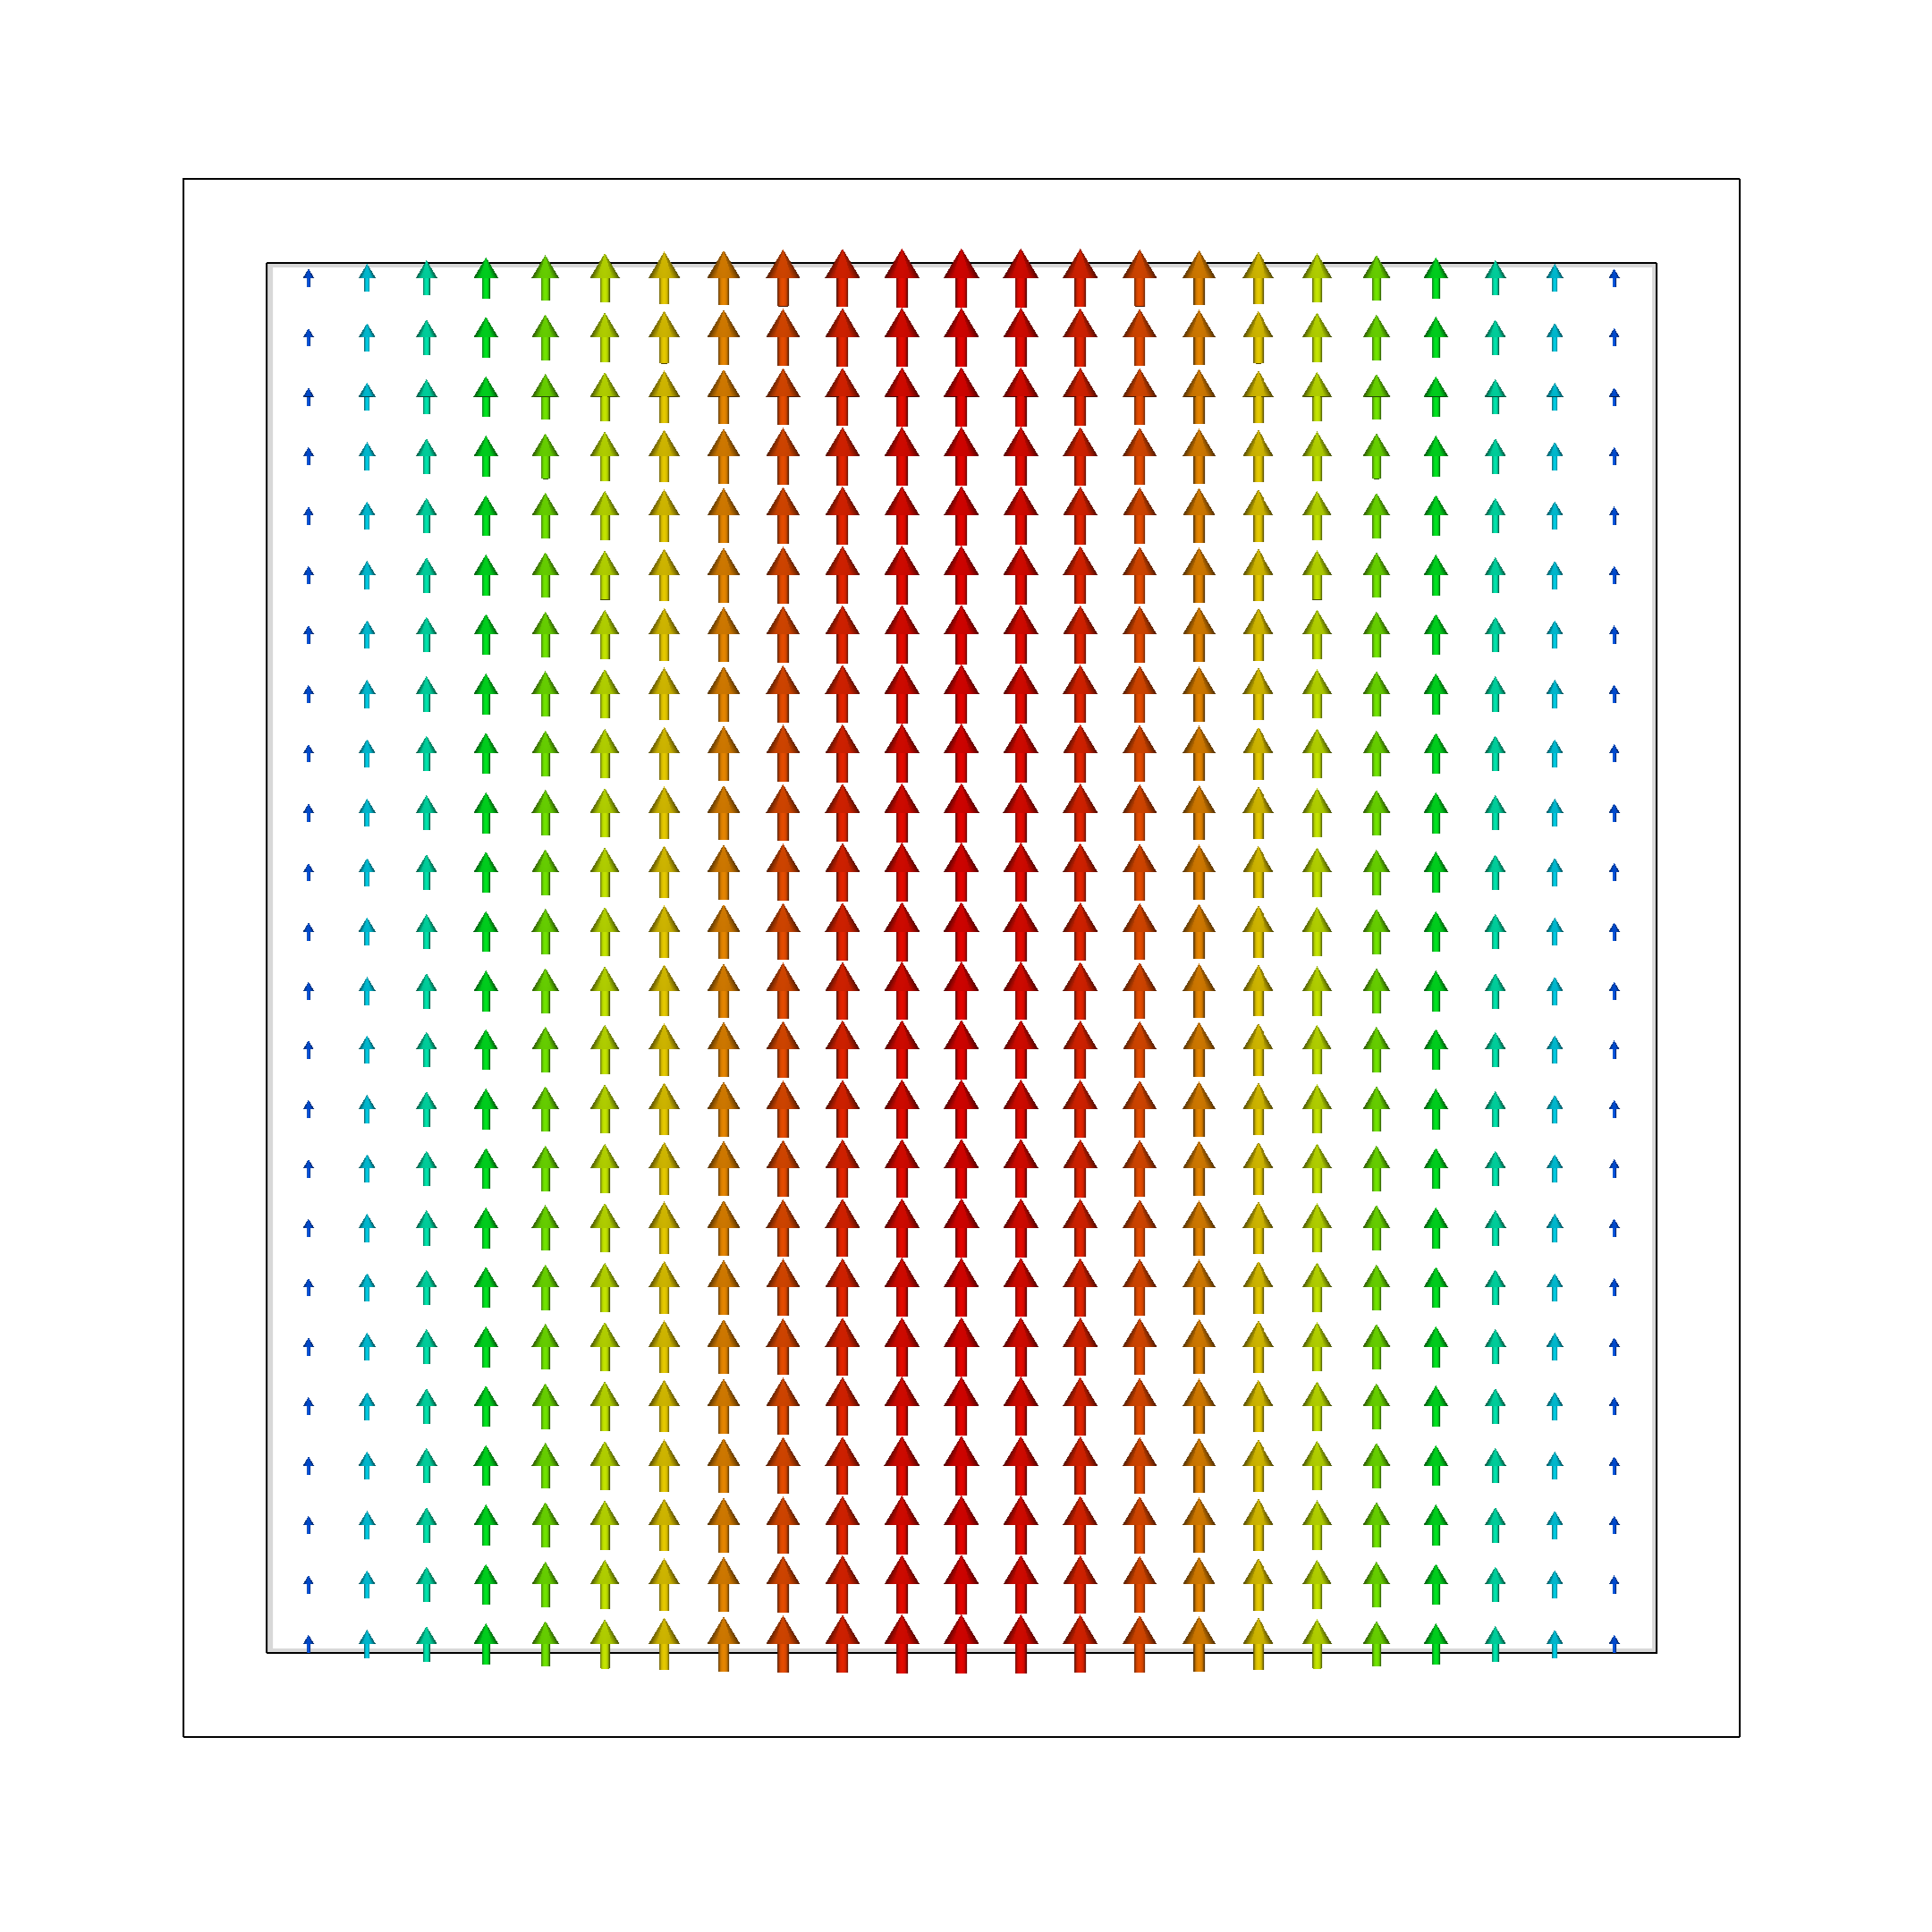
\includegraphics[width=.75\textwidth]{src/waveguide_square_mode2.png}
        \caption{\label{fig:square-waveguide-mode2}}
    \end{subfigure}
    \\
    \begin{subfigure}{.45\textwidth}
        \centering
        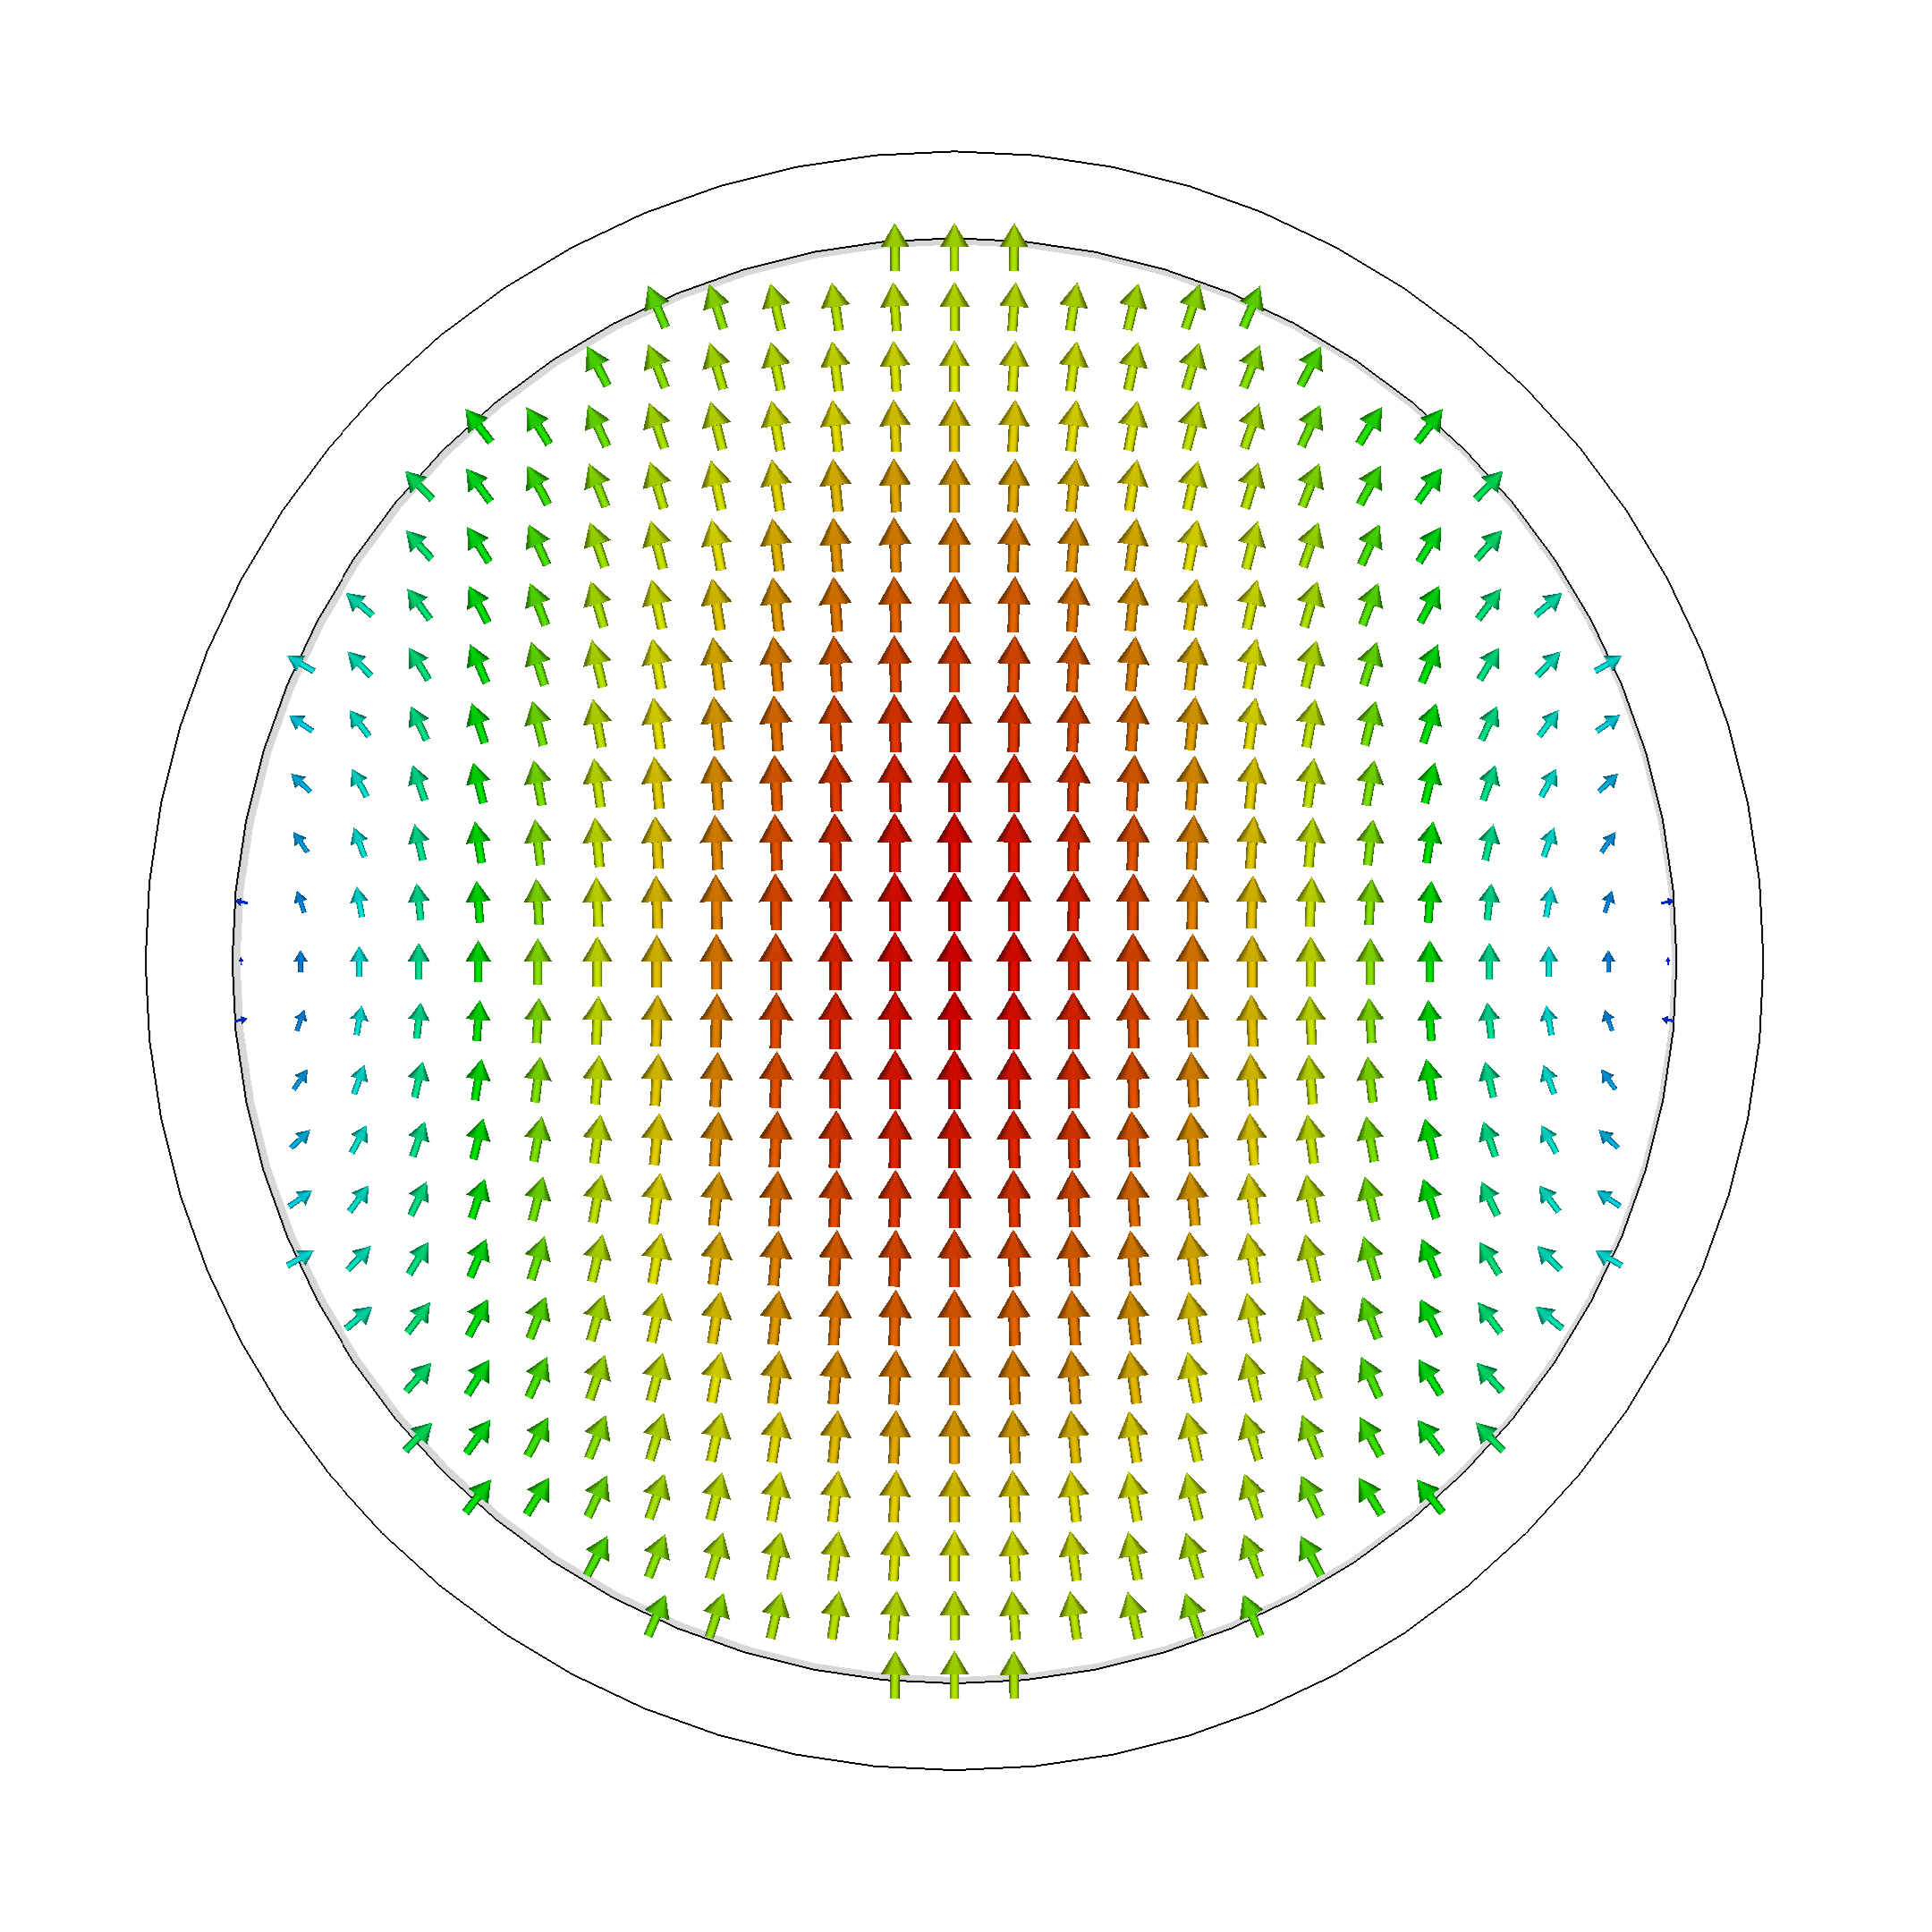
\includegraphics[width=.75\textwidth]{src/waveguide_circular_mode1.png}
        \caption{\label{fig:circular-waveguide-mode1}}
    \end{subfigure}
    \hspace{0.5cm}
    \begin{subfigure}{.45\textwidth}
        \centering
        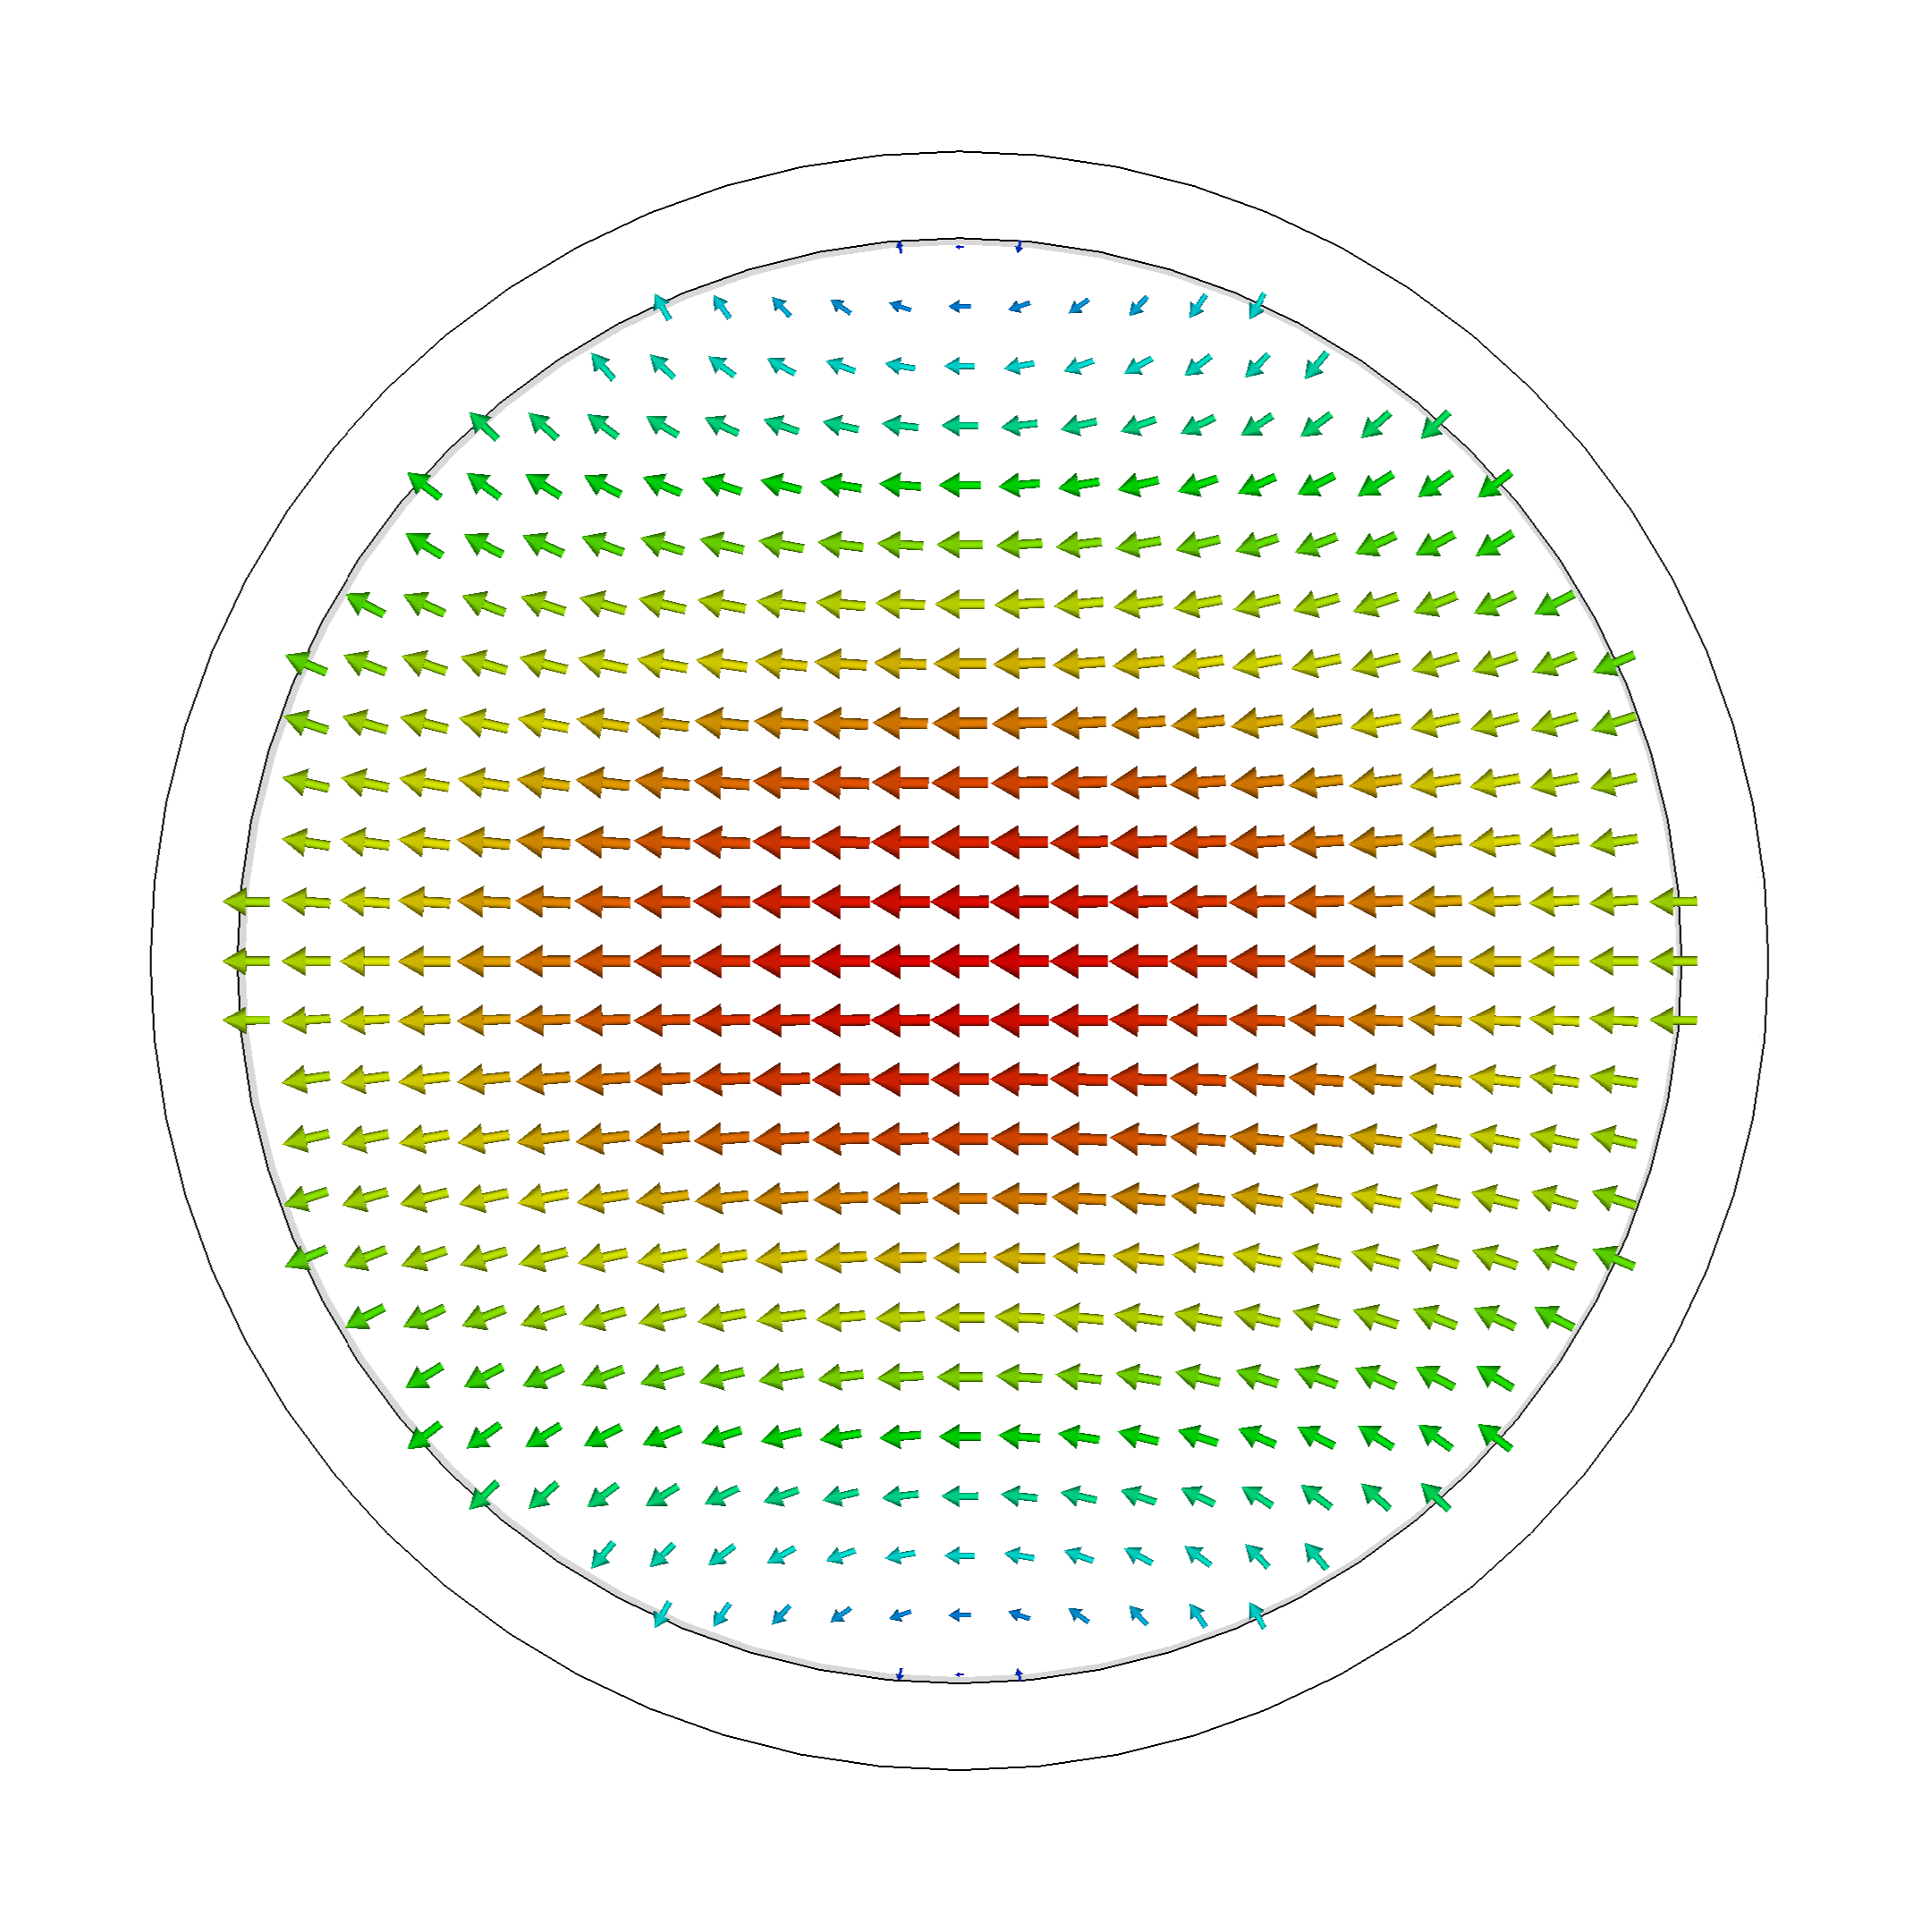
\includegraphics[width=.75\textwidth]{src/waveguide_circular_mode2.png}
        \caption{\label{fig:circular-waveguide-mode2}}
    \end{subfigure}
    \caption{\label{fig:symmetric-waveguide-modes}Symmetric waveguides: fundamental modes}
\end{figure}

\begin{figure}[!ht]
    \centering
    \begin{subfigure}{.45\textwidth}
        \centering
        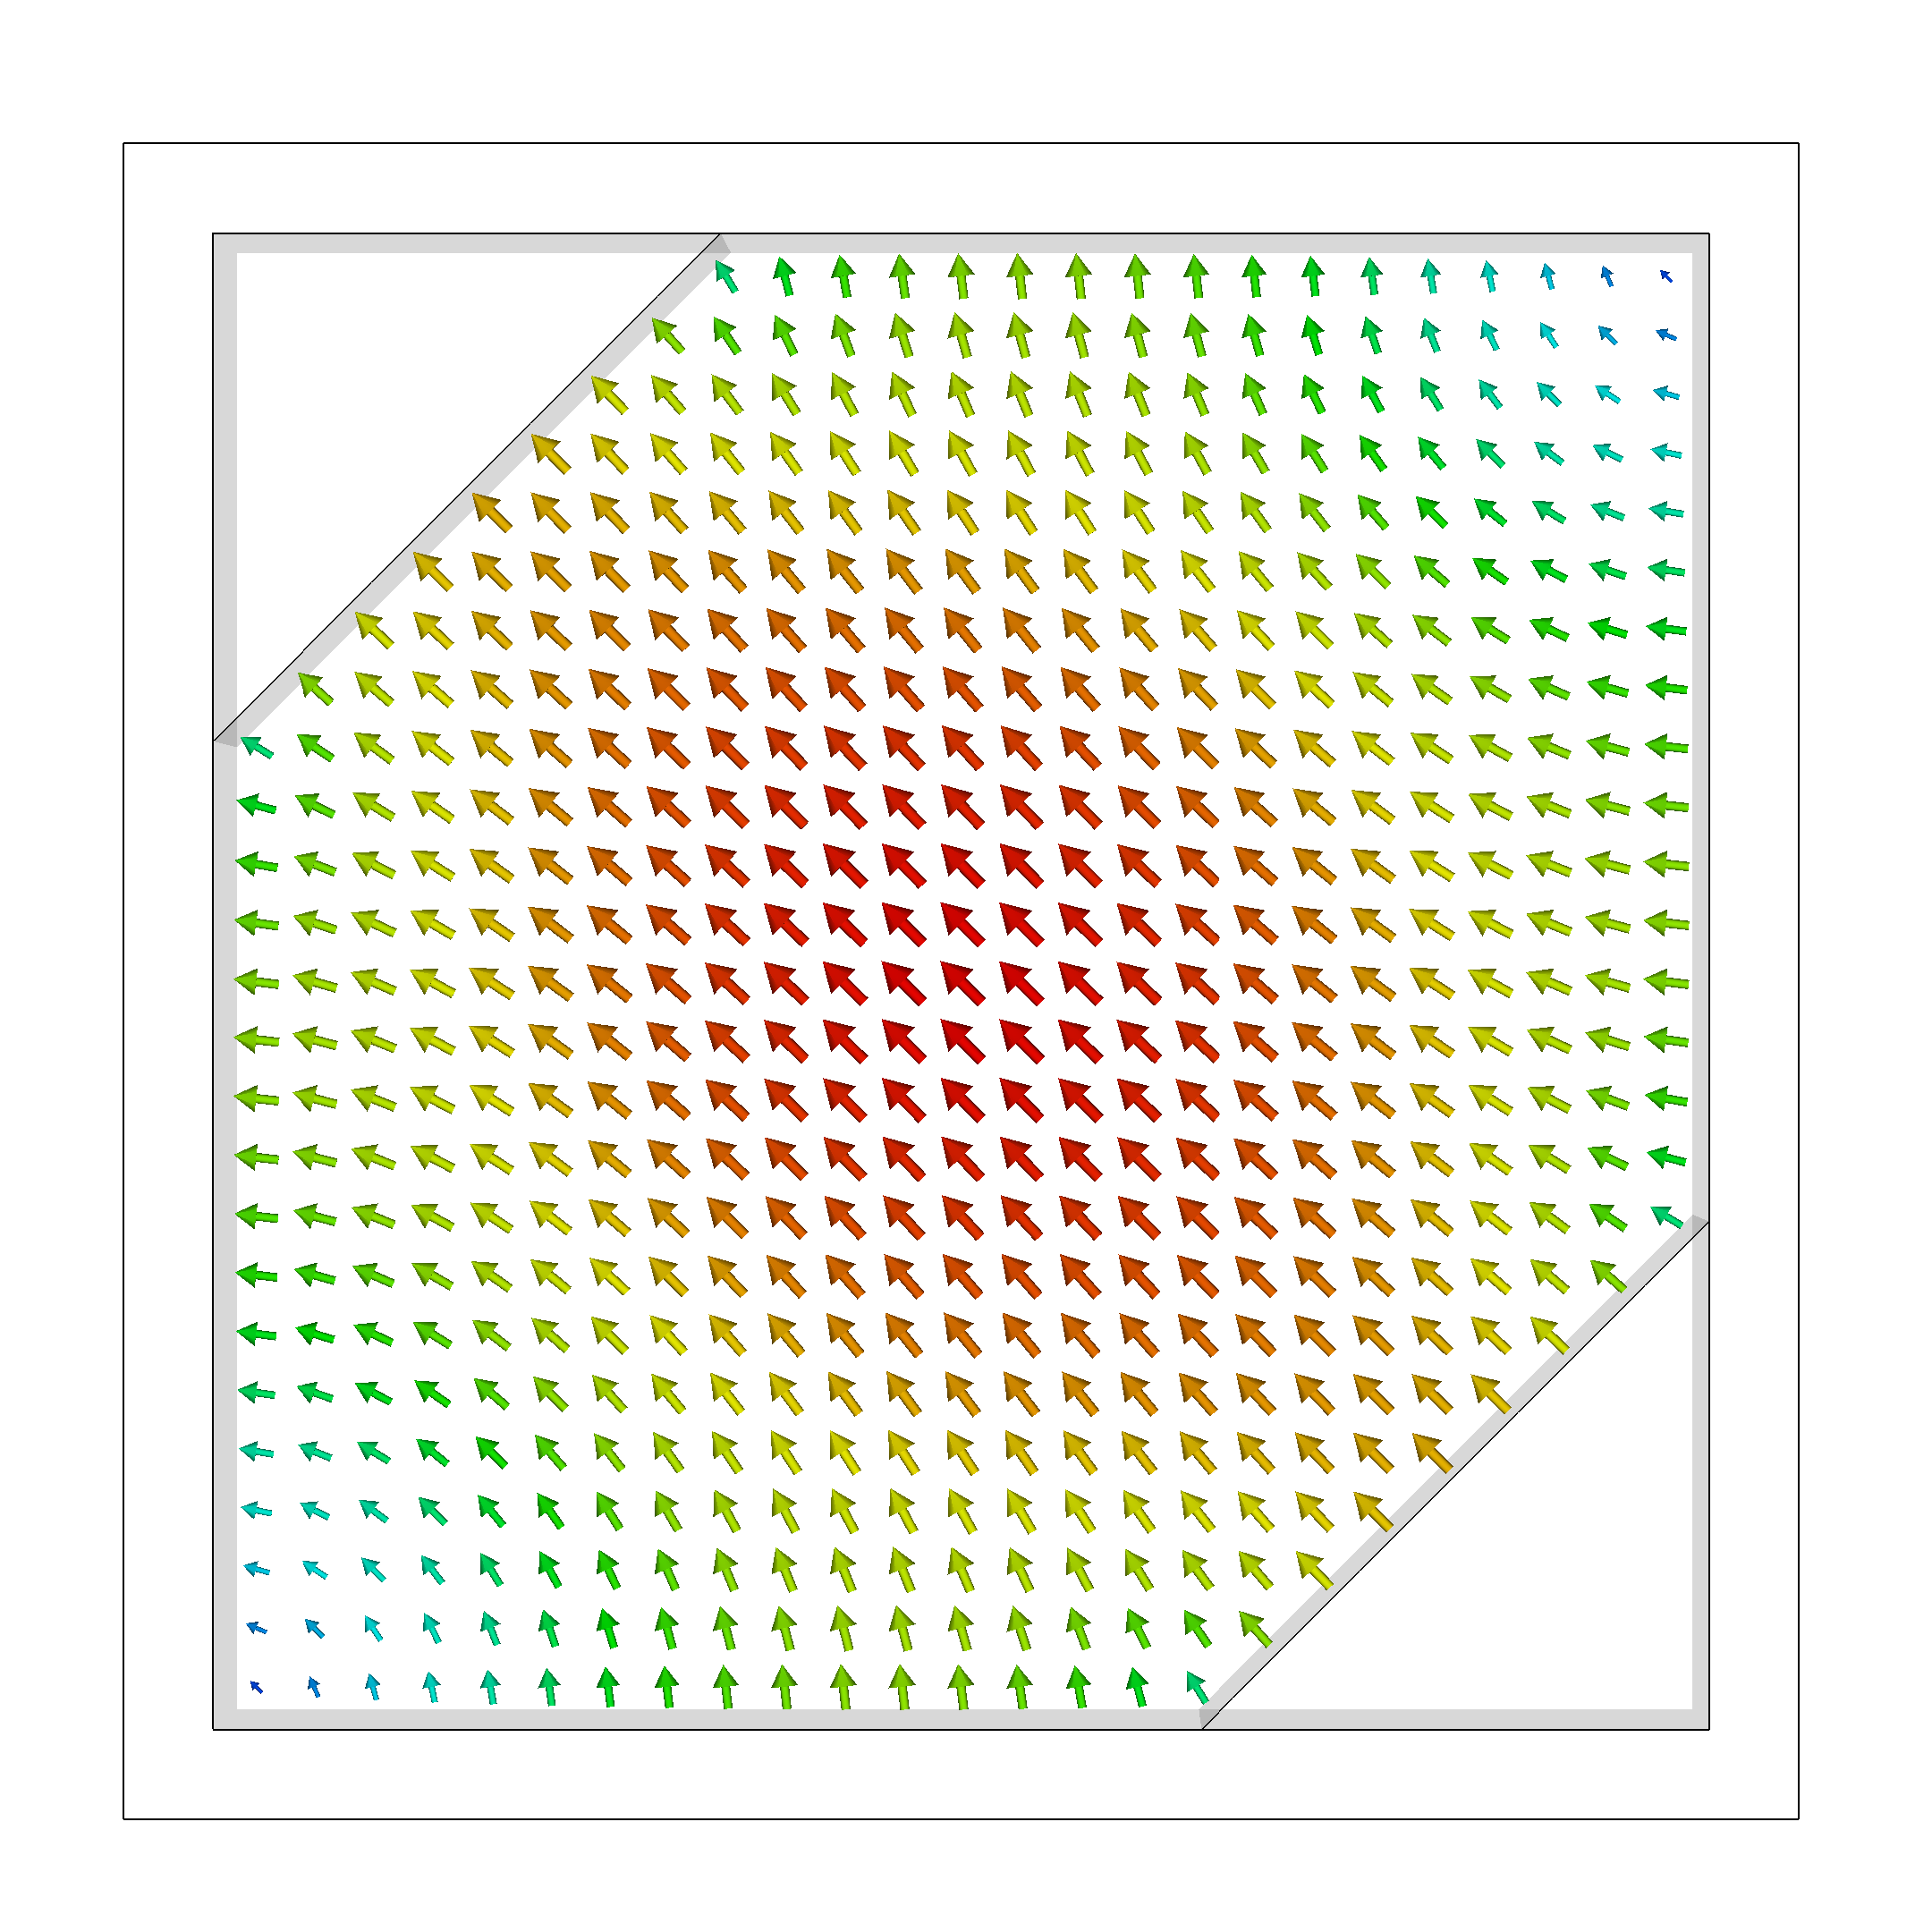
\includegraphics[width=.7\textwidth]{src/polarizer_square_mode1.png}
        \caption{\label{fig:square-polarizer-mode1}}
    \end{subfigure}
    \hspace{0.5cm}
    \begin{subfigure}{.45\textwidth}
        \centering
        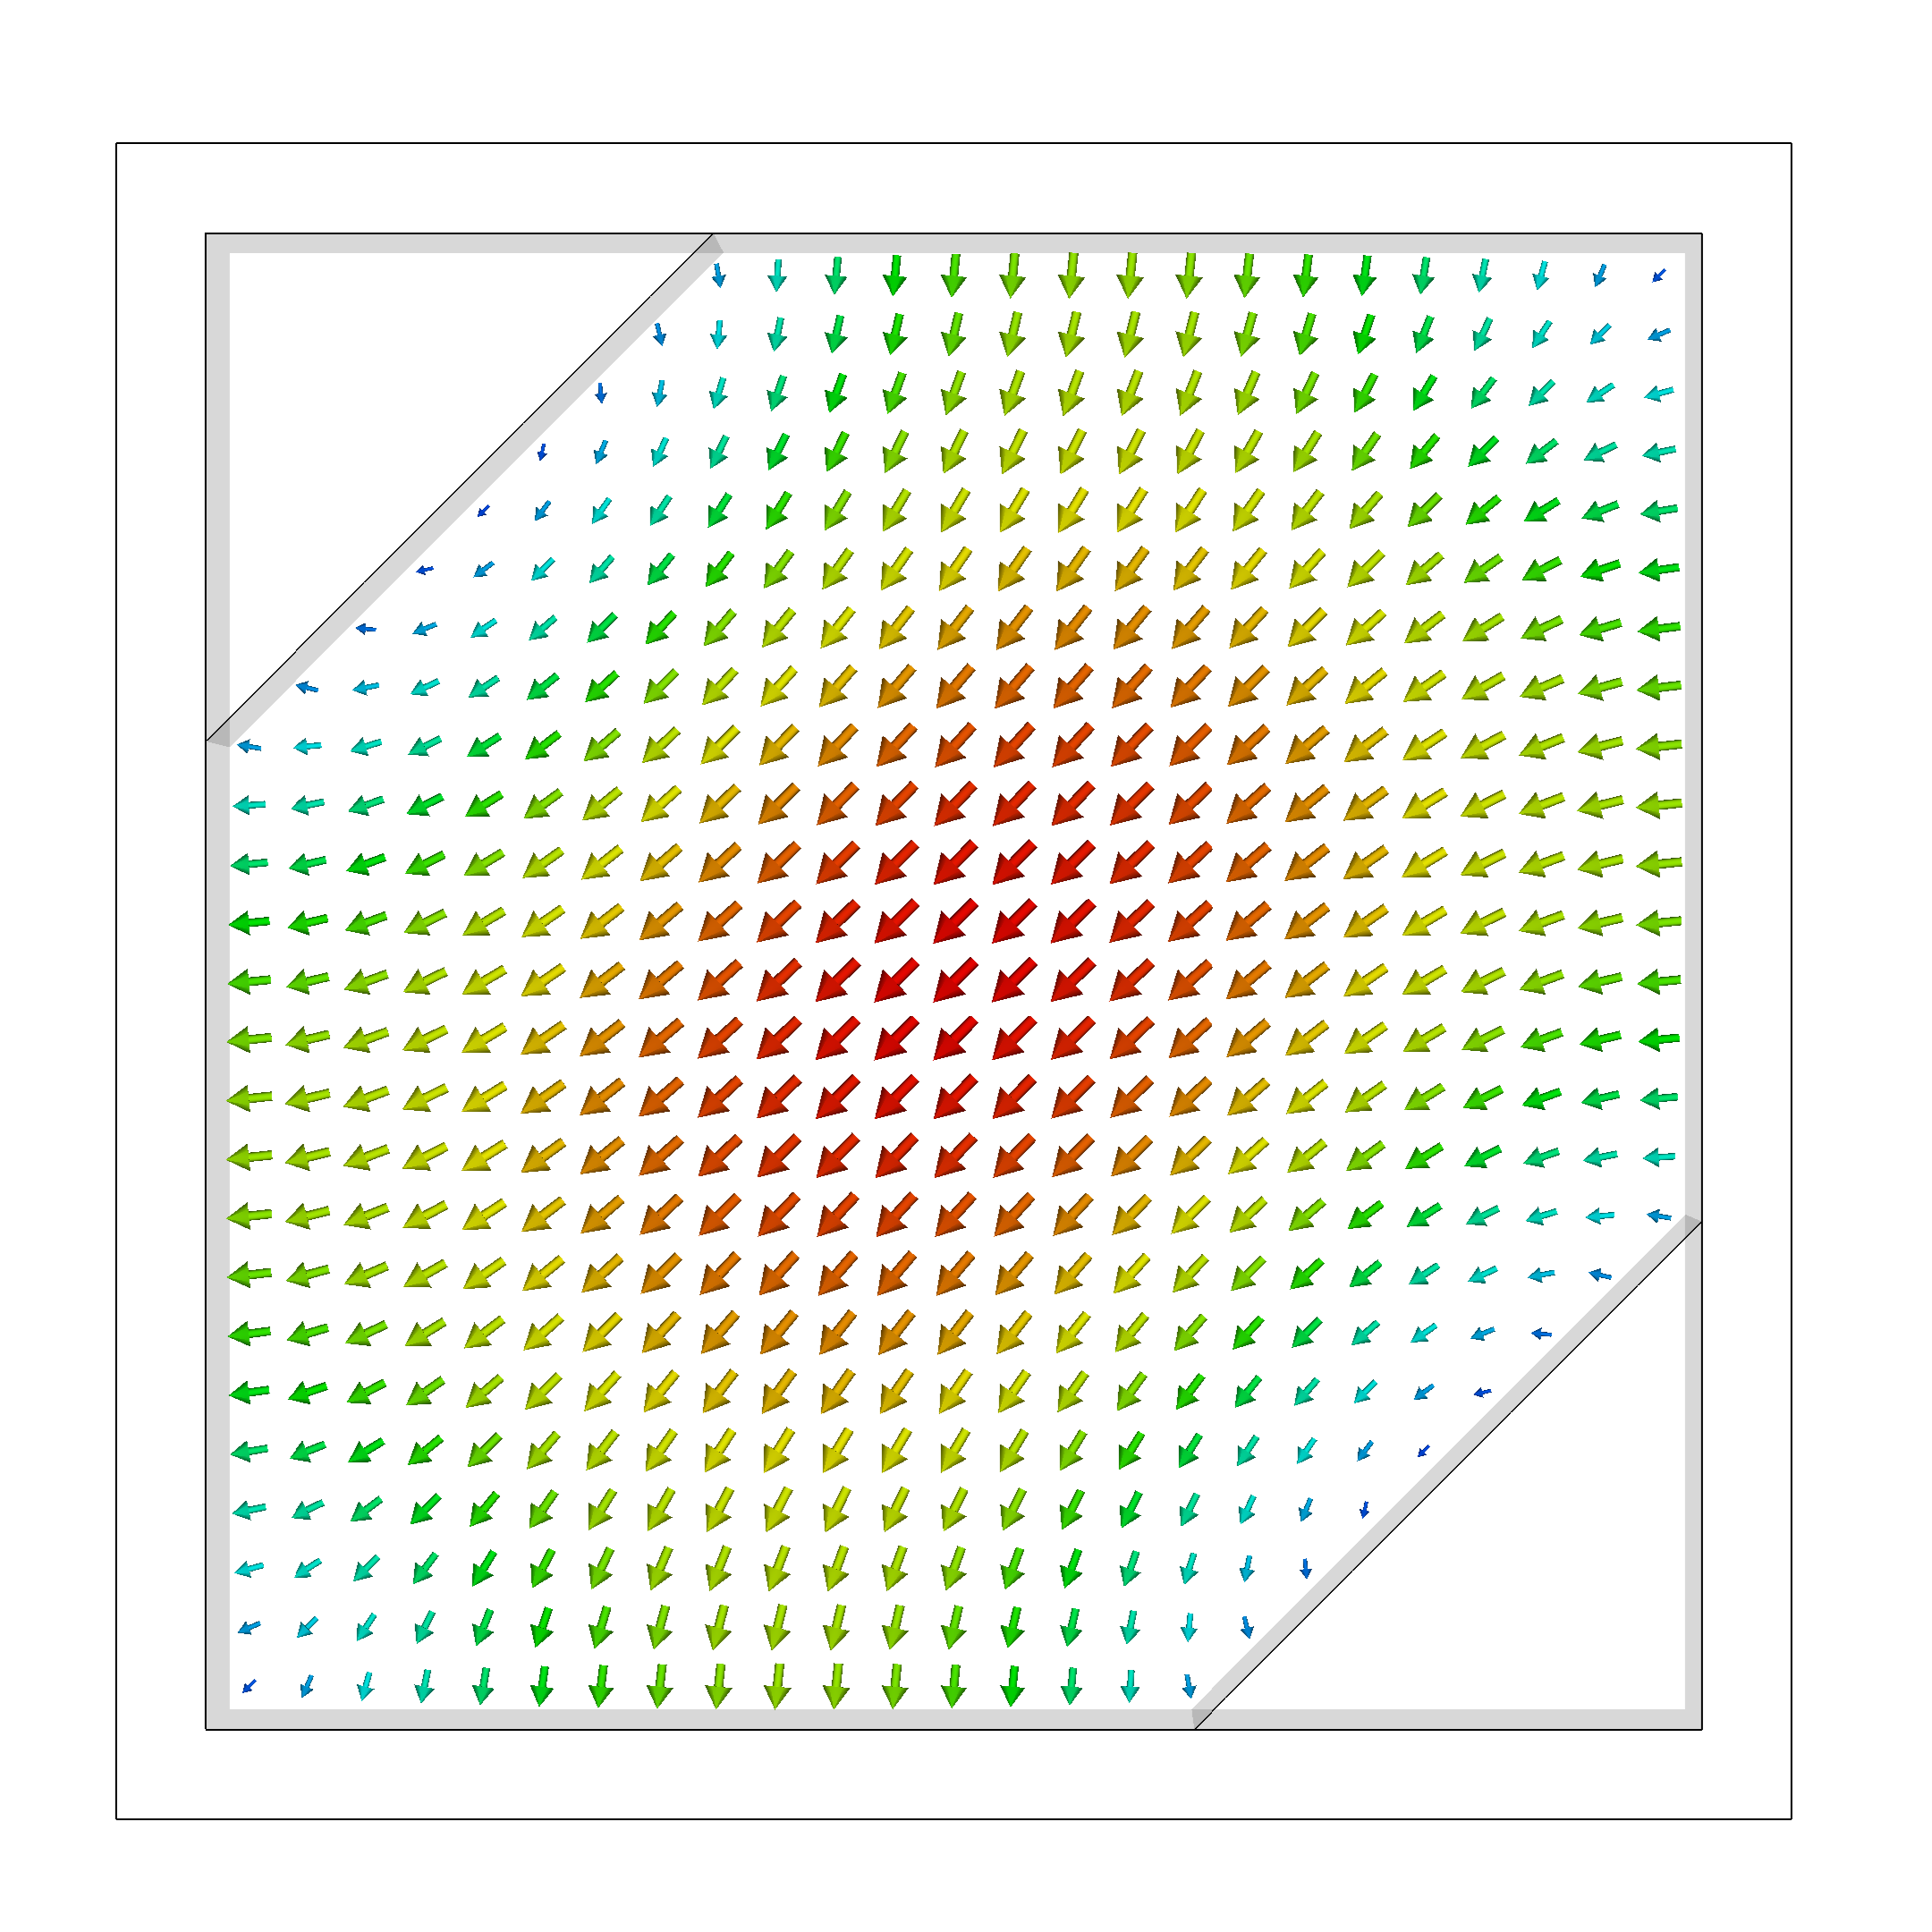
\includegraphics[width=.7\textwidth]{src/polarizer_square_mode2.png}
        \caption{\label{fig:square-polarizer-mode2}}
    \end{subfigure}
    \\
    \begin{subfigure}{.45\textwidth}
        \centering
        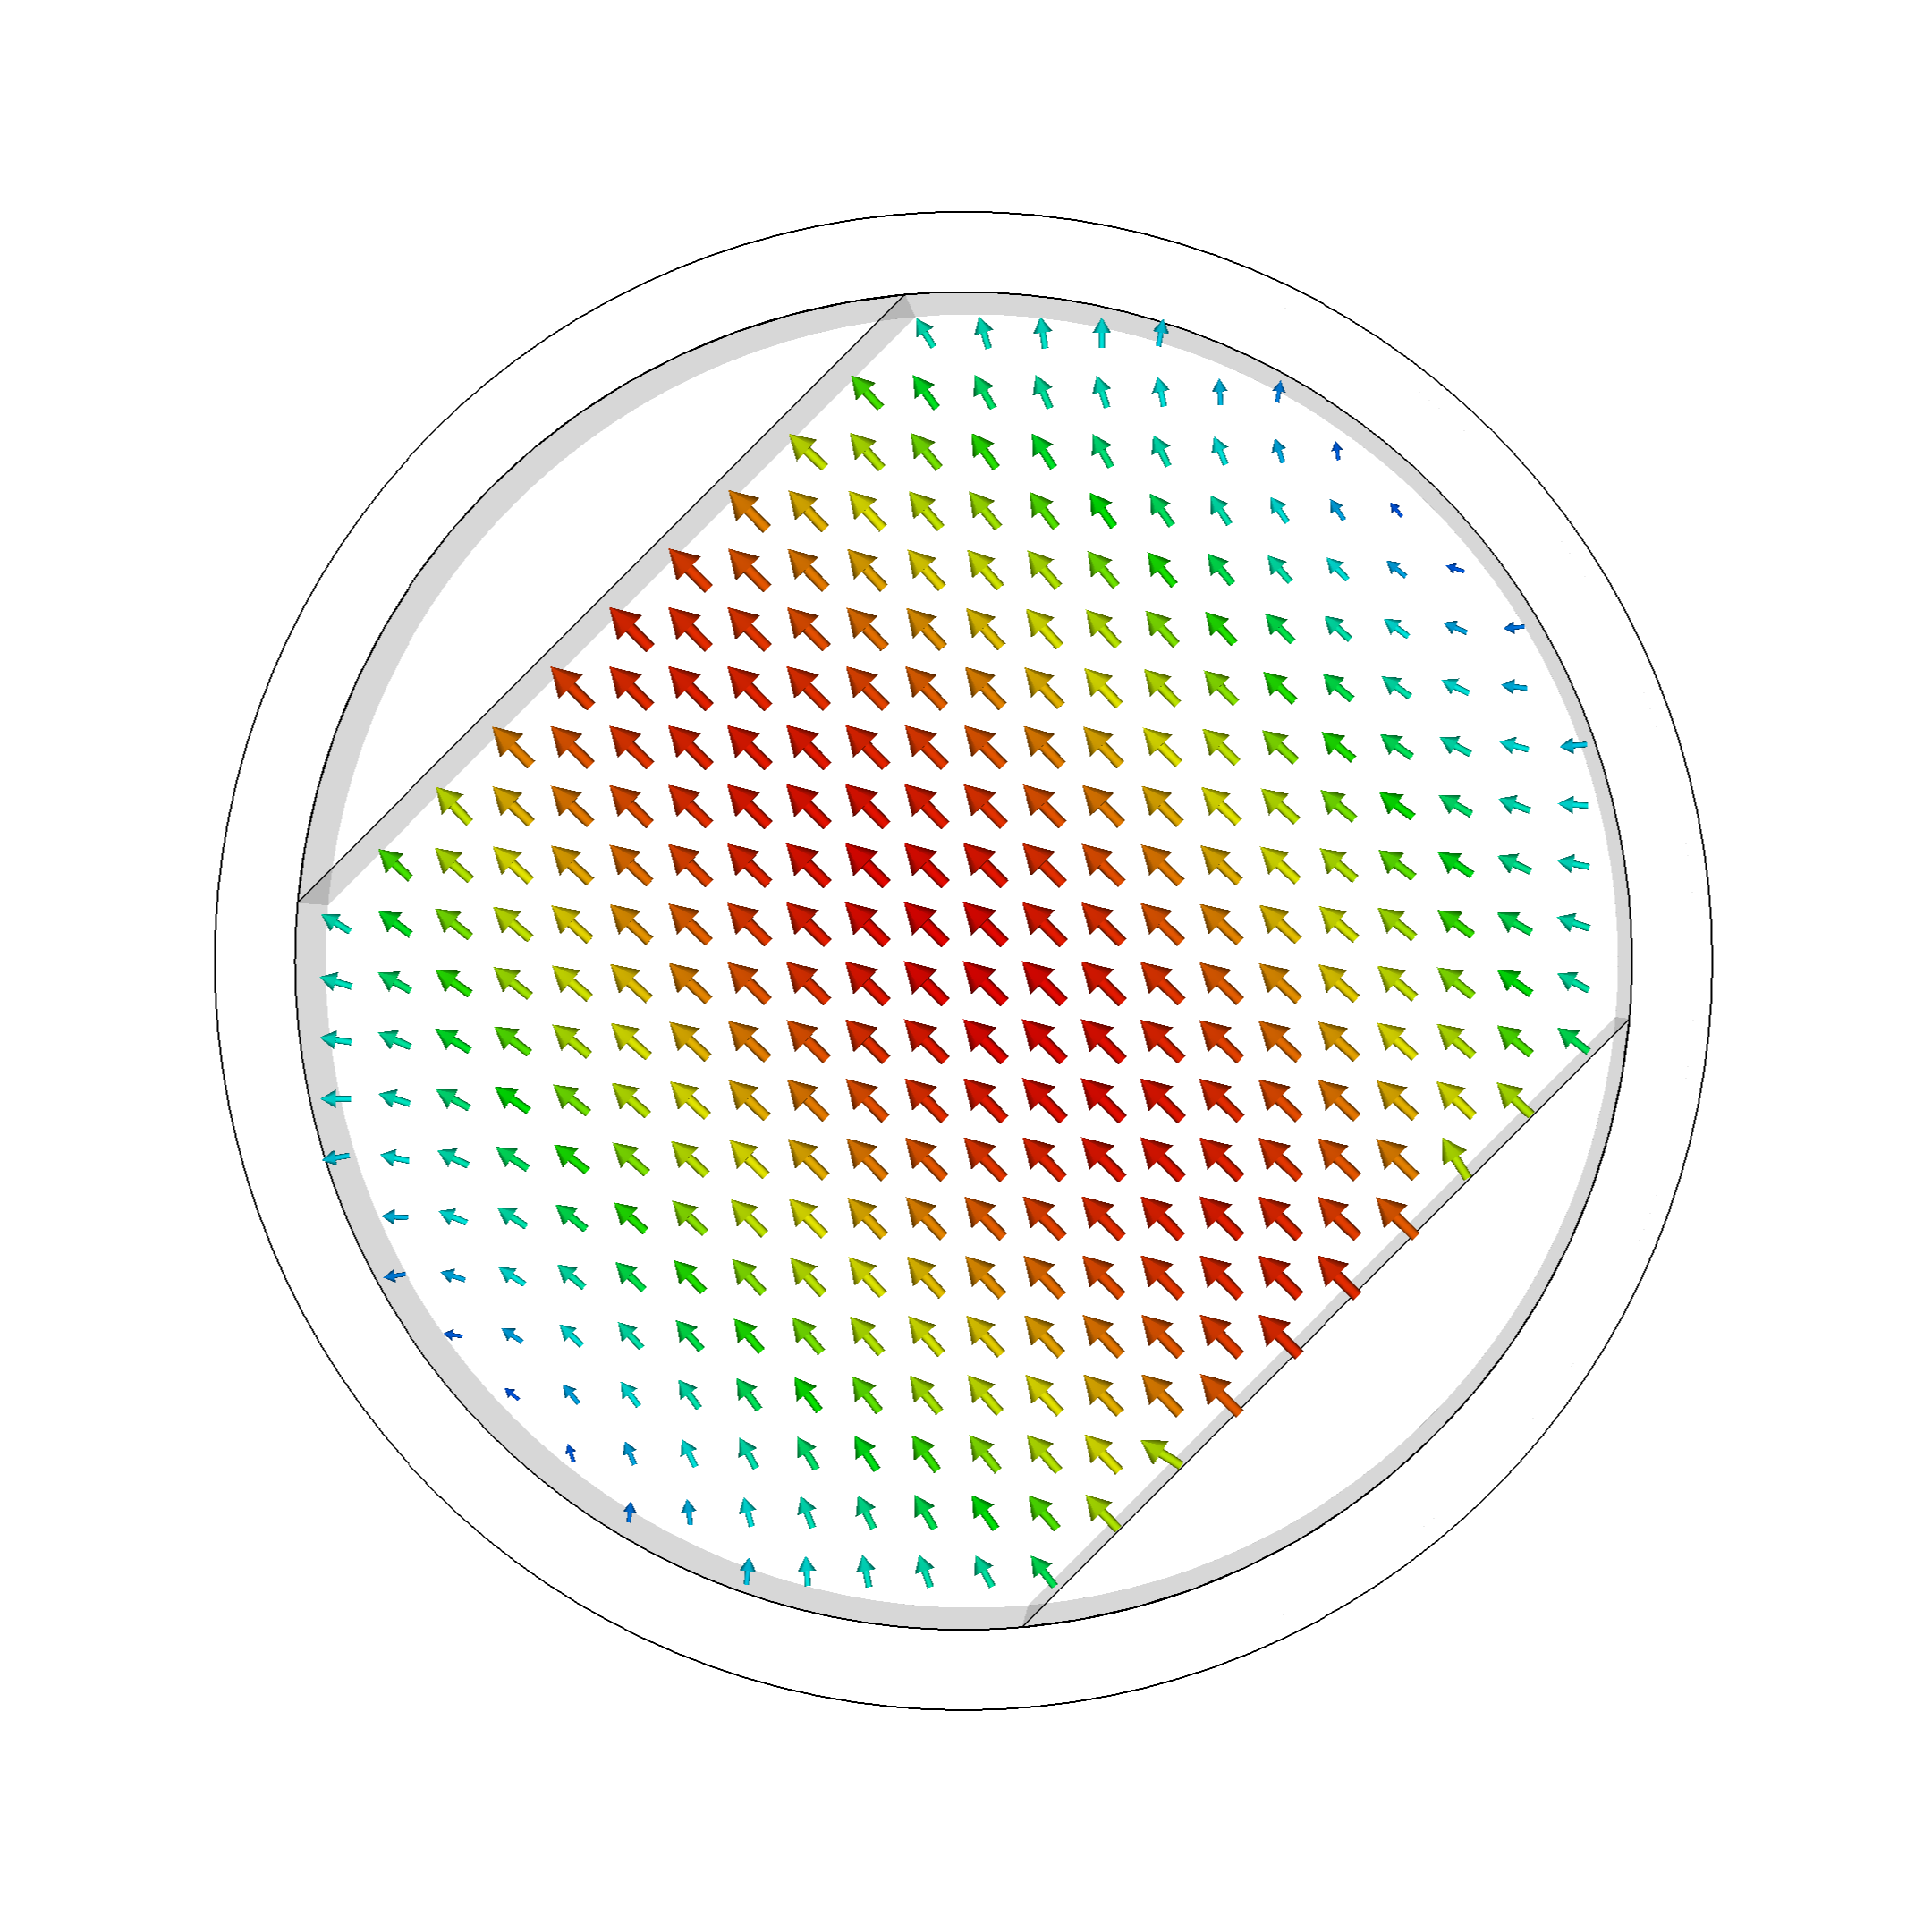
\includegraphics[width=.75\textwidth]{src/polarizer_circular_mode1.png}
        \caption{\label{fig:circular-polarizer-mode1}}
    \end{subfigure}
    \hspace{0.5cm}
    \begin{subfigure}{.45\textwidth}
        \centering
        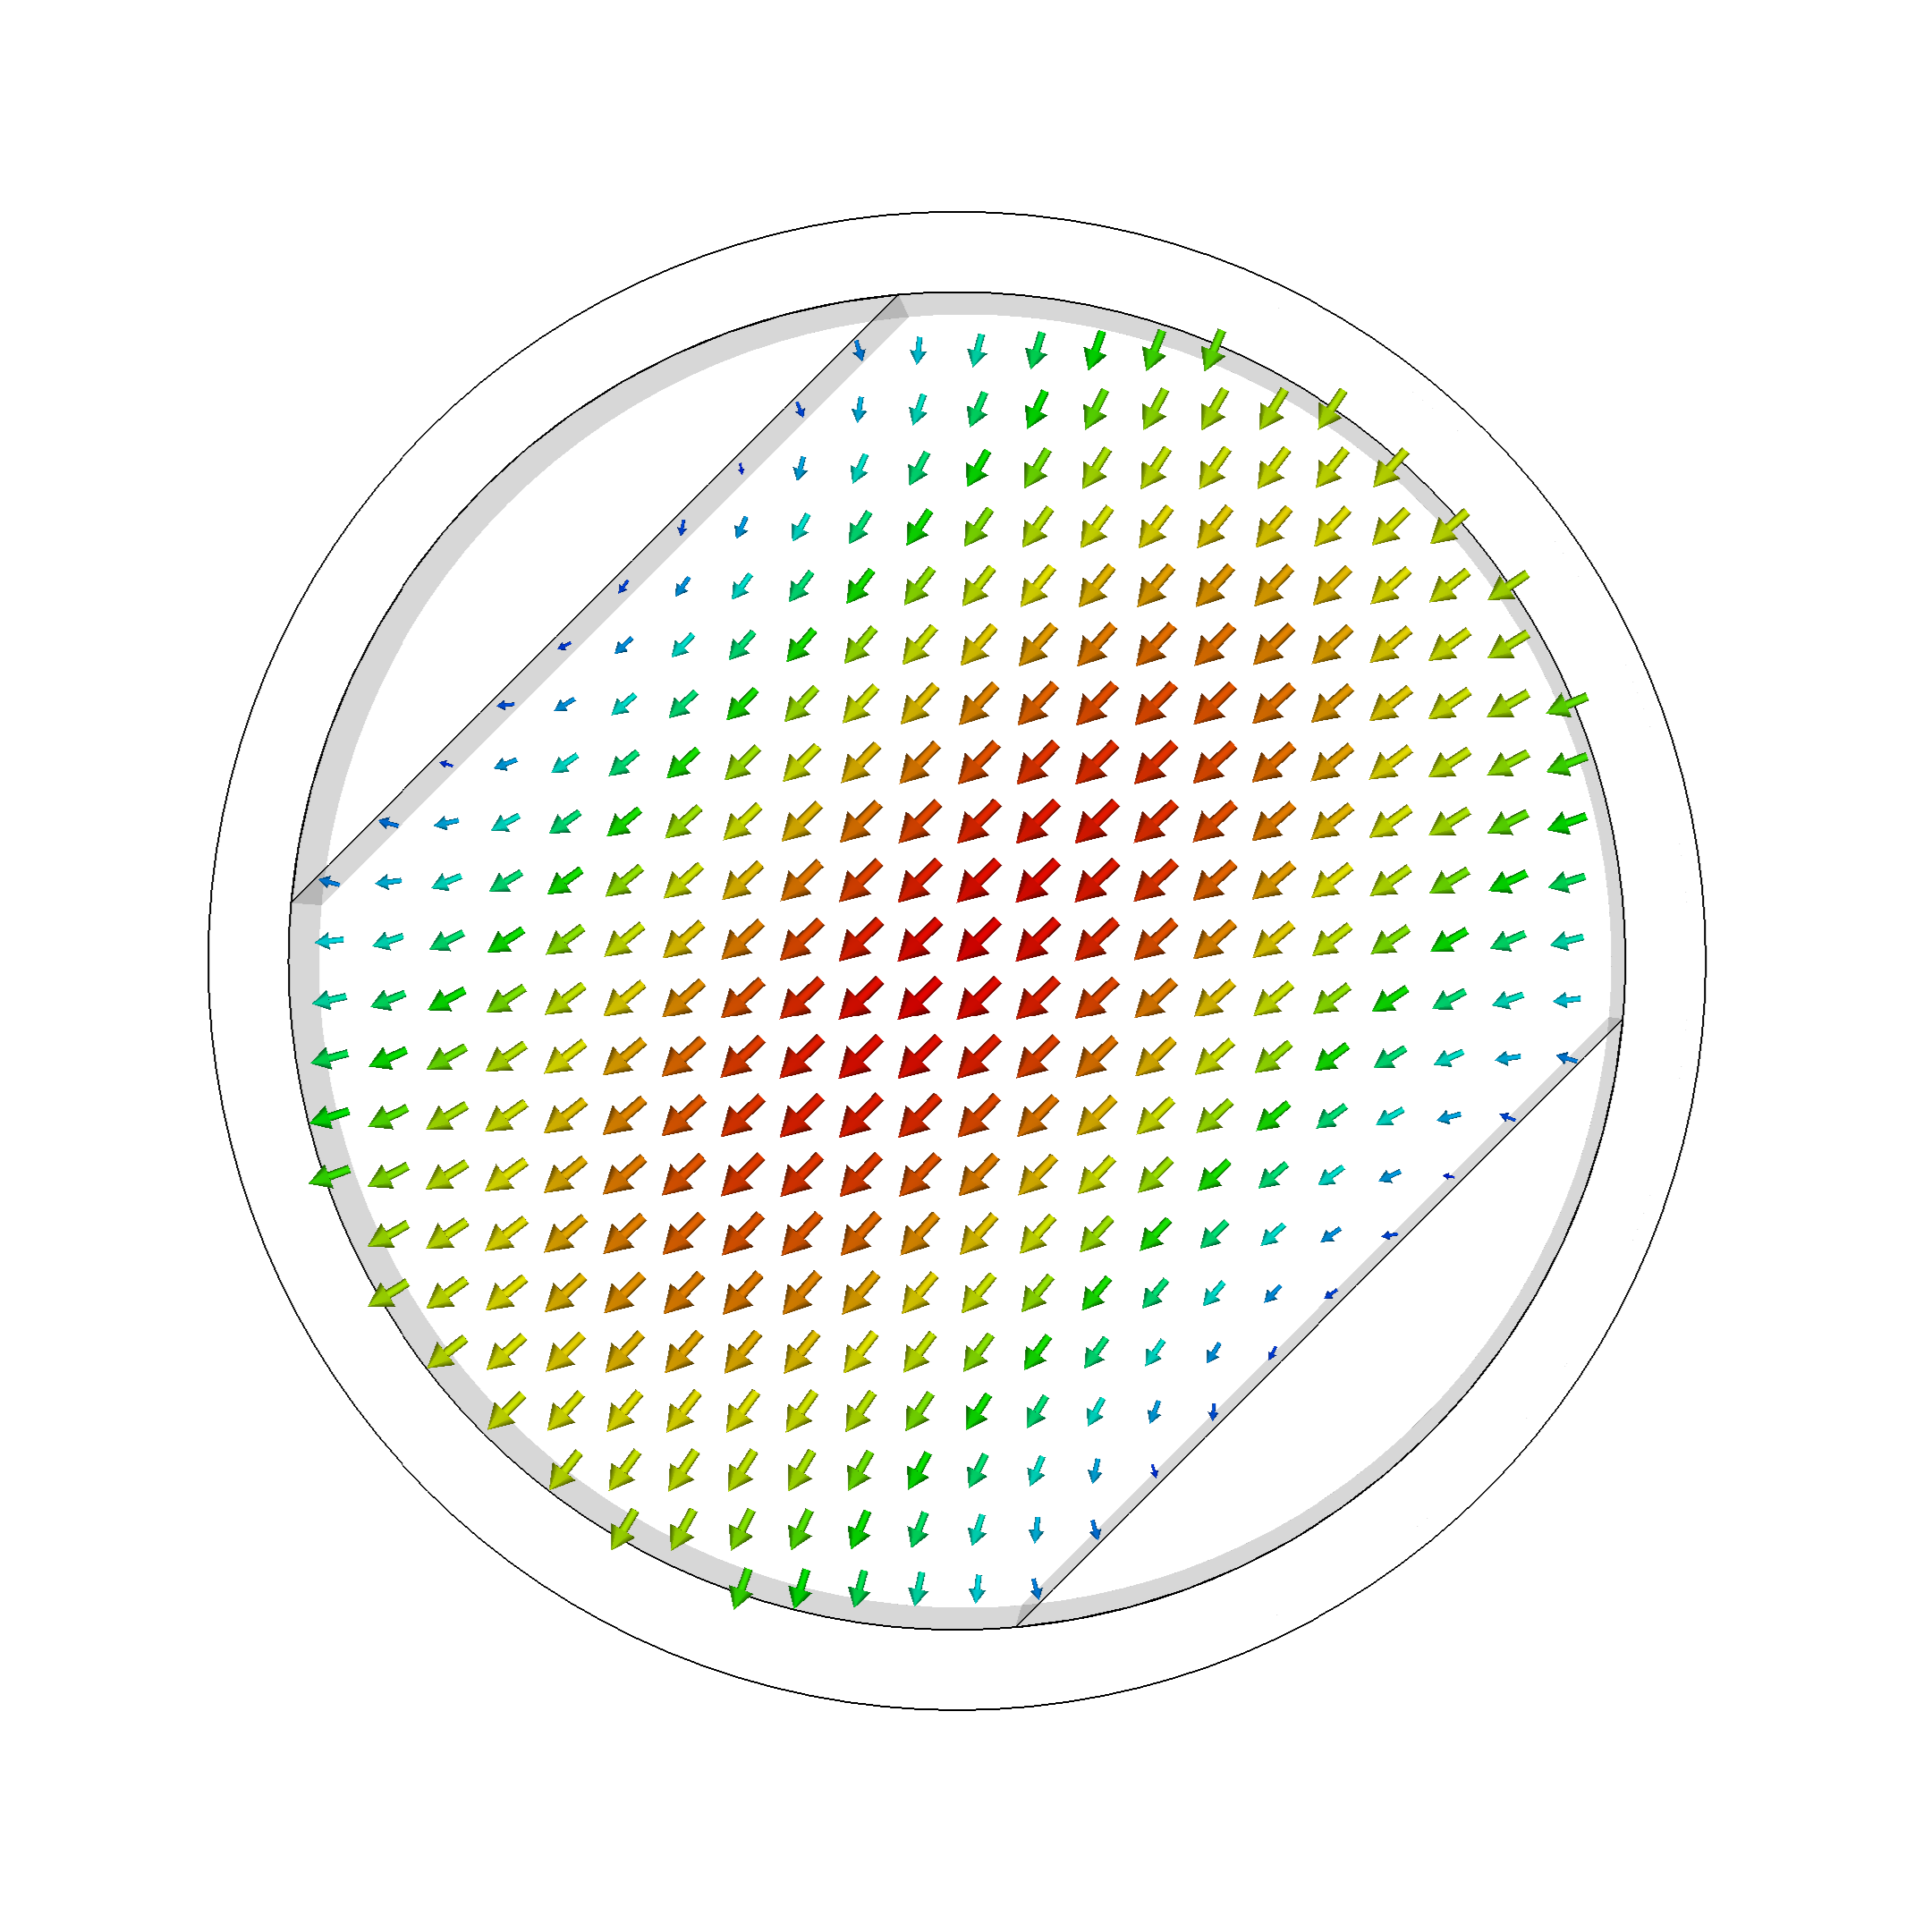
\includegraphics[width=.75\textwidth]{src/polarizer_circular_mode2.png}
        \caption{\label{fig:circular-polarizer-mode2}}
    \end{subfigure}
    \caption{\label{fig:symmetric-polarizer-modes}Symmetric polarizers: fundamental modes}
\end{figure}

With the basic modes established, the eigenmodes of the polarizers, i.e., the same waveguides but now \emph{with} the shapes inserted, are analysed. The eigenmodes take the form presented in \cref{fig:square-polarizer-mode1,fig:square-polarizer-mode2} for the square geometry, whereas the circular waveguide with inserts supports two fundamental modes depicted in \cref{fig:circular-polarizer-mode1,fig:circular-polarizer-mode2}. As expected, in both cases, the transverse field exhibits a standing wave behaviour as dictated by the boundary conditions on a conductive surface. More importantly for the polarization transformation, the metallic shapes perturb the electromagnetic fields, leading to a change in the propagation constants of the existing modes. Crucially, the presence of these inserts breaks the original symmetry of the waveguide, causing a dispersion, or difference in phase velocity, between the two fundamental modes of propagation. This fact is illustrated in \cref{fig:symmetric-polarizer-modes}, where in both geometries, one of the modes perceives a different electric path than the other. This dispersion is the key mechanism for achieving circular polarization. As the electromagnetic wave propagates along the waveguide, the phase difference between the two fundamental modes accumulates. By carefully selecting the geometry and placement of the inserts, as well as the length of the waveguide, this cumulative phase lag can be precisely controlled. In the context of a polarizer designed to generate circular polarization, the goal is to achieve exactly one-quarter wavelength phase difference between the two modes at the output. As shown in \cref{eq:polarization-circular-condition}, this quadrature phase relationship, combined with equal amplitudes of the two modes, results in the generation of a circularly polarized wave. The eigenmode analysis allows for the accurate determination of the modal field distributions, enabling precise design and optimization of the polarizer to achieve the desired phase shift and polarization state.

\begin{remark}[Dual polarization capability]
    \label{remark:dual-polarization-capatibility}
    It is important to note that, with respect to the diagonal symmetry of the polarizer, one of its eigenmodes is always antisymmetric. This means that if exciting the square-waveguide-based polarizer with the $\TE 01$ results in a RHCP, the $\TE 10$ must result in LHCP, or vice versa. This principle can be visualized as decomposing the incident waves from \cref{fig:square-waveguide-mode1,fig:square-waveguide-mode2} into the basis formed by polarizer eigenmodes depicted in \cref{fig:square-polarizer-mode1,fig:circular-polarizer-mode2}: While the horizontal waveguide mode (\cref{fig:square-waveguide-mode1}) can be expressed as a simple sum of the two polarizer modes, the vertical waveguide mode (\cref{fig:square-waveguide-mode2}) requires the negative%
        \footnote{A positive sum of the two eigenmodes is equivalent to the plus sign option in \cref{eq:polarization-circular-e-r0}, as the condition on circular polarization expressed in \cref{eq:polarization-circular-condition} is fulfilled due to the two eigenmodes oscillating perpendicular to each other, i.e., $\delta = \pi/2$. Conversely, adding one eigenmode to the negative of the other introduces an additional $\pi$ to the phase difference $\delta$. The condition for circular polarization is again fulfilled, but with $\delta = 3\pi/2$, causing the sine in \cref{eq:polarization-circular-e-r0} to take a negative value, resulting in the opposite circular polarization.}
    of the antisymmetric polarizer mode (\cref{fig:square-polarizer-mode2}). Although this principle was illustrated using the square waveguide structure, the same holds true for the circular geometry with its two orthogonal degenerate modes (\cref{fig:circular-waveguide-mode1,fig:circular-waveguide-mode2}). This unique property enables the structures to produce dual circular polarization simply by switching between two excitations.

    Furthermore, due to the mirror symmetry of both polarizers, optimizing the structure with respect to just a single orientation of circular polarization is sufficient. By the essence of the matter, the other polarization must retain the same performance parameters, as will be proven by simulation.
\end{remark}

\subsection{Figures of merit}
A crucial outcome of the eigenmode analysis is the gained insight into the operational principles, which helps define relevant variables and performance parameters intrinsic to the structure's geometry, ultimately aiding in polarizer optimization. The optimization process aims to produce circular polarization while minimizing production costs, primarily by reducing the polarizer length, $L$. This necessitates maximizing the \emph{specific mode phase shift}, given by
\begin{align}
    \label{eq:polarizer-specific-phase-shift}
    \Delta k_L(f) &= \frac 1L \int_0^L \[k_2-k_1\](z,f)\,\d z,
\end{align}
where $k_1$ and $k_2$ are the propagation constants of the two polarizer modes and $z$ is the Cartesian coordinate aligned with the propagation direction. This quantity represents the average difference in propagation constants between the two modes along the polarizer,%
    \footnote{This quantity is analogous to the birefringence effect observed in optics, where a material exhibits different refractive indices for different polarizations, causing a phase difference to accumulate between them as they propagate. Here, the waveguide structure, due to its geometry, effectively creates different propagation constants for the two orthogonal modes, leading to a similar effect.}
effectively quantifying the rate at which the phase difference between them accumulates as they propagate. However, \cref{eq:polarizer-specific-phase-shift} addresses only one of the two conditions for circular polarization \eqref{eq:polarization-circular-condition}, the other being the requirement for equal mode amplitudes:
\begin{align}
    \label{eq:polarizer-amplitude-ratio}
    \left.\frac{E_2}{E_1}\right|_{z=L} = 1,
\end{align}
where $E_1$ and $E_2$ are the amplitudes of the two modes and the polarizer output. A weighted aggregate of \cref{eq:polarizer-specific-phase-shift,eq:polarizer-amplitude-ratio} forms the objective function of the optimization problem, with the variables being the geometric parameters of the polarizer cross-section. Intuitively, larger inserted shapes induce a greater phase lag per unit length but also introduce larger amplitude distortions between the modes. This reveals an inherent conflict within the problem, necessitating a trade-off. From an application perspective, a balance must be struck between the length of the structure, which compensates for a lower phase delay per unit length, and polarization purity, which is compromised by unequal mode magnitudes.

\subsection{Comparison of symmetric waveguides}
\label{subsection:comparison-of-symmetric-waveguides}
To conclude the eigenmode analysis, a decision will be made, using the previously introduced figures of merit, regarding which geometry is better suited for polarization control, considering both practical and performance aspects. Ideally, minimal frequency dependence of both figures, \cref{eq:polarizer-specific-phase-shift,eq:polarizer-amplitude-ratio}, is desired. However, due to the inherently resonant operational principle of the waveguide, achieving feasible performance across an ultrawide band with a single section of such a polarizing structure is not considered possible.

Before proceeding, the practical evaluation of \cref{eq:polarizer-specific-phase-shift,eq:polarizer-amplitude-ratio}  should be addressed. Given that both polarizers are analysed as uniform waveguides (\cref{fig:polarizer-square-perspective,fig:polarizer-circular-perspective}), the propagation dispersion between the two modes, and consequently both metrics, can be approximated as constant throughout the polarizer, i.e., $\partial_z\Delta k_L=0$. This approximation allows \cref{eq:polarizer-specific-phase-shift} to be expressed as
\begin{align}
    \label{eq:polarizer-phase-shift}
    \Delta k_L(f) &= \[k_2-k_1\](f)
\end{align}
and the overall mode phase shift at the polarizer output is given by
\begin{align}
    \Delta\phi(f) &= L\[k_2-k_1\](f).
\end{align}

Furthermore, this simplification permits the evaluation of both \cref{eq:polarizer-amplitude-ratio,eq:polarizer-phase-shift} from a single reading at the polarizer output. For this purpose, an \emph{$E$-field probe} functionality within CST Studio Suite can be utilized, allowing the magnitude and phase of the electric field to be determined at a specified point in space, evaluated across all frequencies. Consequently, the objective function for maximum specific phase shift, \cref{eq:polarizer-specific-phase-shift}, is transformed into the minimization of
\begin{align}
    \label{eq:polarizer-length-for-90deg}
    L_\perp(f) &= \frac\pi4\frac{L}{\Delta\phi(f)}
\end{align}
representing the polarizer length required to achieve a mode phase shift of $\pi/4$.%
    \footnote{It is important to note that, due to phase wrapping, the cross-section tuning simulations must be
    conducted for a polarizer shorter than that required to produce a $\pi/4$ phase shift.}
This modified objective function can be readily computed using the \emph{Template-Based Post-Processing} feature within CST Studio Suite, using $\Delta\phi(f)$ obtained from the $E$-field probe result. Moreover, the practical feasibility of the polarizer is inherently incorporated into this formulation.

To facilitate a fair comparison, the two polarizers depicted in \cref{fig:polarizer-square-perspective,fig:polarizer-circular-perspective} are modelled with a similar cutoff frequency. For an operating band of $\frequencyrange$, a diameter of $\qty{50}{mm}$ for the circular waveguide and a side length of $\qty{50}{mm}$ for the square waveguide are selected. This selection results in a cutoff frequency of approximately $\qty{3}{GHz}$ for both underlying waveguides. As previously discussed, both polarizer metrics, \cref{eq:polarizer-amplitude-ratio,eq:polarizer-length-for-90deg}, are predominantly influenced by the cross-sectional geometry. Consequently, both polarizers have been parameterized by the width, $w$, of their chamfering inserts, as depicted in \cref{fig:polarizer-square-perspective,fig:polarizer-circular-perspective}.

\begin{figure}[!ht]
    \centering
    \includesvg[width=\textwidth]{src/polarizers_cutoff_frequencies.svg}
    \caption{\label{fig:polarizers-cutoff-frequencies}Polarizers: cutoff frequencies}
\end{figure}

\begin{figure}[!ht]
    \centering
    \includesvg[width=\textwidth]{src/square_polarizer_cross_section.svg}
    \caption{\label{fig:square-polarizer-cross-section}Square polarizer: cross-section tuning}
\end{figure}

\begin{figure}[!ht]
    \centering
    \includesvg[width=\textwidth]{src/circular_polarizer_cross_section.svg}
    \caption{\label{fig:circular-polarizer-cross-section}Circular polarizer: cross-section tuning}
\end{figure}

The mode cutoff frequency dispersion in \cref{fig:polarizers-cutoff-frequencies} is observed to be similar for both polarizers. However, a comparison of \cref{fig:square-polarizer-cross-section,fig:circular-polarizer-cross-section} reveals that superior phase dispersion is achieved by the square waveguide, while maintaining a lower amplitude dispersion gradient. Henceforth, this text concerns the design of a square waveguide polarizer, and the simple term \emph{polarizer} will therefore refer to this specific kind.

\section{Square waveguide polarizer}
With the fundamental waveguide structure established, the complete polarizer design can now be elaborated upon. This section outlines the design procedure, including all key considerations and design choices made. The process begins by defining the design requirements, which will serve as the foundation for modelling the structure.

\paragraph{Selection of parameters.} The first step in the design process was to define the operating band. A frequency band spanning from $\frequencyrange$ was selected for this polarizer. This range was chosen to cover common applications in satellite communication and radar systems.

Based on this frequency range, the initial dimensions of the square waveguide were determined. As outlined in \cref{subsection:comparison-of-symmetric-waveguides}, the corresponding side length of $\qty{50}{mm}$ was selected for the square waveguide. This value was inspired by the commercially available WR-187 rectangular waveguide,
    \footnote{Also known as WG12 in the RCSC standard and R48 in the IEC standard.}
a standard component with dimensions and frequency range specified in~\parencite{spinner:waveguide-specifications}. However, it is important to note that the insertion of prisms into the square waveguide, a key element of the design, significantly alters the dispersion characteristics compared to a standard rectangular waveguide. Thus, the $\qty{50}{mm}$ value was chosen as a starting point and further refined through simulations.

To confirm the suitability of this dimension, simulations were carried out. The results of these simulations, which were already presented in \cref{fig:polarizers-cutoff-frequencies}, show the cutoff frequencies of the waveguide with the inserted prisms. These cutoff frequencies are critical as they define the operating bandwidth of the waveguide. Based on the simulated cutoff frequencies, it was confirmed that the $\qty{50}{mm}$ side length provided an appropriate operating bandwidth for the target frequency range of $\frequencyrange$.

With the side length established, the next step involved determining the dimensions of the chamfering and the overall length of the polarizer. These parameters were determined through a parametric sweep using simulations. This involved systematically varying the chamfering width and observing its impact on the polarizer's performance. The results of this parametric sweep are presented in \cref{fig:square-polarizer-cross-section}.

After a careful analysis of the simulated results, a chamfering width of $\qty{23}{mm}$ and a polarizer length of $\qty{126}{mm}$ were chosen. These values were selected to provide optimal performance with respect to polarization purity, meaning the ability to effectively transform a linearly polarized wave into a circularly polarized one. Additionally, these dimensions maintain a satisfactory axial ratio, which, as represented by the amplitude ratio in \cref{eq:polarizer-amplitude-ratio}, is a critical measure of the quality of the generated circular polarization.

\subsection{Simulation results}
The polarizer design section concludes with an evaluation of the polarizer's performance under full-wave simulation. Previous simulations were limited to analysing the eigenmode properties of the polarizer geometry. Consequently, it remains to be verified that the proposed solution functions as intended, i.e., that a linearly polarized $\TE 01$ or $\TE 10$ wave, guided by a square waveguide (as depicted in \cref{fig:square-waveguide-mode1,fig:square-waveguide-mode2}), is effectively converted into a circularly polarized wave upon excitation of the structure.

To simulate more realistic operating conditions, two sections of standard rectangular waveguide, with the same side length as the polarizer, are introduced at each end of the polarizer structure, as depicted in \cref{fig:polarizer-perspective}. The input waveguide section facilitates the excitation of the polarizer with a linearly polarized wave. The output waveguide section serves as a rudimentary radiating element, allowing for an initial assessment of the radiated field. It also allows for verification that the generated circular wave maintains its integrity during the transition from the polarizer to a subsequent waveguide section, while also minimizing the influence of reflections. This configuration further permits an examination of the radiation characteristics of the open-ended waveguide, providing preliminary insights into parameters such as co-polarization, cross-polarization directivity, and axial ratio, effectively representing a minimalist circularly polarized antenna.

The results, in the form of radiation patterns for co- and cross-polarizations of both incident waveguide modes, are presented in \cref{fig:polarizer-radiation}. Other antenna parameters, such as scattering parameters, are not studied since the antenna in \cref{fig:polarizer-perspective} serves only as a validation of the polarizing functionality. The radiation from an open-ended waveguide, while serving as a valid check of the radiation properties, suffers from large reflections due to the unmatched transition from a waveguide into free space. Perhaps the most important quality factor of circular polarization, the axial ratio, is evaluated in the far-field and is analogous to \cref{eq:polarizer-amplitude-ratio} which describes the ratio of the orthogonal $E$-field components.

\begin{figure}[!ht]
    \centering
    \includegraphics[width=.8\textwidth]{src/polarizer_perspective.png}
    \caption{\label{fig:polarizer-perspective}Final polarizer: model}
\end{figure}

The previous eigenmode analysis is confirmed by these results. As shown in \cref{fig:polarizer-radiation}, the axial ratio maintains a low value (with values below $<\qty{3}{dB}$ generally being considered acceptable), even reaching $\qty{0}{dB}$ around the centre of the design band. The elevation radiation patterns are displayed at centre frequency.

\begin{figure}[!ht]
    \centering
    \includesvg[width=\textwidth]{src/polarizer_radiation.svg}
    \caption{\label{fig:polarizer-radiation}Final polarizer: radiation properties}
\end{figure}

\chapter{Feeding structure}
\label{chapter:feeding-structure}
This chapter details the design of a transition from two coaxial cables into a square waveguide, with each cable exciting only one of the fundamental $\TE 01$ and $\TE 10$ modes propagating within the waveguide. This facilitates an excitation of the polarizer, detailed in \cref{chapter:polarizer}, equivalent to the artificial excitation used during the polarizer simulations, which were performed using a dual-mode waveguide port in CST Studio Suite.

The initial design considers the well-established problem of a single coaxial-to-waveguide transition employing a right-angled probe within the waveguide cavity. Following an evaluation of the single-feed adapter's performance, the feasibility of introducing a second feed into the same cavity is assessed, and the challenges posed by this are recognized. A solution, involving separating the two excitation ports by a grating polarizer, enabling their mutual displacement, is adopted. This approach offers significant potential for reducing the mutual probe coupling below the margin of measurement error. Finally, simulation data are presented to demonstrate the performance of the final structure.

\section{Coaxial-to-waveguide transition}
\label{section:coaxial-to-waveguide-transition}
The problem of coaxial-to-waveguide transition is well-established and rudimentary, with a vast body of existing research available, such as~\parencite{fabregas-et-al:coaxial-to-rectangular-waveguide-transitions}. These transitions most frequently employ a \emph{right-angle transition}%
    \footnote{While there is also the option to feed the waveguide \emph{in-line}, i.e., by leading the coaxial cable's inner conductor through the adapter back wall, this technique is infeasible for the problem at hand. Apart from the obvious challenge of implementing this solution in a dual-feeding scheme, the in-line transition is known to generally perform in a narrower band, be prone to higher reflections, exhibit mode impurities in the waveguide, and pose a more difficult manufacturing challenge due to its use of a \enquote{shorting elbow} or other auxiliary constructions.}
due to its ease of implementation and tuning, especially when compared to alternative solutions, such as the in-line transition described in~\parencite{durga-et-al:millimiter-wave-inline-coaxial-to-rectangular-waveguide-transition}. In this work, the simplest implementation is adopted, realized by a simple protrusion of the feeding cable's inner conductor through a side wall. The protruding conductor forms a radiating dipole element, exciting the waveguide with the carried wave. As with dipole antennas, this solution is expected to be relatively narrowband. Various methods exist to extend the bandwidth of low reflection, such as loading the dipole element with a metallic disc or cylinder, or forming a conical widening at the probe's end. However, since the polarizer is already expected to operate in a limited band, such modifications are not considered in this thesis, trading the potential bandwidth benefits for enhanced ease of manufacturing.

\begin{figure}[!ht]
    \sbox\twosubbox{%
        \resizebox{\dimexpr.95\textwidth-1em}{!}{%
            \includegraphics[height=3cm]{src/single_feed_side_cut_view.png}%
            \includegraphics[height=3cm]{src/single_feed_front_view.png}%
        }%
    }
    \setlength{\twosubht}{\ht\twosubbox}

    \centering
    \subcaptionbox{\label{fig:single-feed-side-cut-view}Side-cut view}{
        \includegraphics[height=\twosubht]{src/single_feed_side_cut_view.png}
    }\quad
    \subcaptionbox{\label{fig:single-feed-front-view}Front view}{
        \includegraphics[height=\twosubht]{src/single_feed_front_view.png}
    }
    \caption{\label{fig:single-feed-model}Single feed: section views}
\end{figure}

The performance of a single right-angle transition, also called an $E$-plane transition, as illustrated in \cref{fig:single-feed-model}, depends crucially on the precise tuning of two key parameters: the probe length, denoted by $l_1$, and its distance from the \enquote{back-short}, denoted by $d_1$. This section will focus on determining the optimal values of these parameters to achieve efficient power transfer within the dominant $\TE 10$ mode.

Design guidelines typically suggest a probe length of half the waveguide's narrow dimension. Considering that rectangular waveguides are generally built with a $2:1$ side length ratio,%
    \footnote{The wider dimension $A$ is typically chosen to be $3\lambda/4$ at the centre frequency as fundamental $\TE 10$ mode propagation is limited by the lower mode cutoff, occurring for $\lambda=2A$, and the higher mode cutoff, for $\lambda = A$. Consequently, utilizing the $2:1$ ratio, the narrow dimension is $3\lambda/8$.}
the suggested probe length is given by
\begin{align}
    \label{eq:probe-length}
    l_1 &= \frac{3}{16}\lambda_{\mathrm c},
\end{align}
where $\lambda_{\mathrm c}$ is the centre wavelength. The probe acts similarly to a monopole antenna radiating into the waveguide. For optimal radiation, a monopole antenna's length should be somewhat smaller than one-quarter of the operating wavelength, due to the deviation from the idealized elementary dipole model, which assumes an infinitely thin conductor. Furthermore, the analogy is not perfect due to the presence of the waveguide walls and the influence of fringing capacitance at the probe tip. Consequently, the empirical value presented in \cref{eq:probe-length} aligns well with the theory of monopole antenna radiation as the working principle of the transition.

Since the monopole radiates omnidirectionally the half-space above the waveguide wall, a significant portion of the input power is directed towards the back-short. The distance to this shorting wall, $d_1$, is therefore primarily determined by the requirement for constructive interference of the wave reflected by the back-short with the waves emanating from the probe in the desired direction. To understand this, consider the wave propagation within the dominant $\TE 10$ mode. The back-short, acting as a conductive, hence a highly reflective, wall, introduces a phase shift of $\pi$ upon reflection. For constructive interference, the total phase shift experienced by the wave during its round-trip journey from the probe to the back-short and back to the probe must be an integer multiple of $2\pi$. The simplest solution that satisfies the constructive interference requirement is to set the back-short distance to one-quarter of the guide wavelength.%
    \footnote{The relevant wavelength in this scenario is the guide wavelength, $\lambda_g$, which represents the wavelength of the propagating wave within the waveguide under the dominant $\TE 10$ mode. This is distinct from the free-space wavelength $\lambda$, as detailed in \cref{example:te-waves-in-a-rectangular-waveguide}, and is given by \cref{eq:guide-wavelength}.}
Consequently, the probe's distance to the back-short can be expressed as
\begin{align}
    \label{eq:probe-distance}
    d_1 &= \frac{\lambda_{\mathrm g}}{4} = \frac{\lambda}{4\sqrt{1-\(\dfrac{\lambda}{\lambda_{mn}}\)^2}},
\end{align}
where the cutoff wavelength $\lambda_{mn}$, corresponding to the cutoff frequency from \cref{eq:cutoff-frequency}, can be simplified as $2A$, where $A$ is the waveguide side length.

\begin{remark}
    \label{remark:probe-distance-higher-order-resonances}
    While constructive interference theoretically occurs for any probe distance $d_1 = (2\nu+1)\pi$, where $\nu\in\N_0$ (i.e., any odd-integer multiple of $\pi$), the quality factor of such resonances rapidly increases with distance, thus resonant wavelength. Consequently, higher-order resonances ($\nu > 0$) exhibit impractically narrow bandwidths and are highly sensitive to dimensional variations, such as engineering tolerances during the fabrication process, making them unsuitable for reliable operation. Therefore, the fundamental resonance ($\nu = 0$) is preferred for practical $E$-plane transition designs.
\end{remark}

\paragraph{Single feed tuning.} This section concludes with the optimization of the single-port adapter parameters. Unlike the polarizer tuning, design guidelines are now available, providing reasonable initial estimates. These values, in conjunction with well-defined objective functions, are utilized as the starting point for a multi-variable optimization. The primary objective is the efficient transfer of energy from the coaxial TEM mode to one of the fundamental waveguide modes ($\TE 01$ or $\TE 10$); therefore, the objective function is defined as the minimization of port reflection ($S_{11}$).

Initial values for $d_1$ and $l_1$, calculated from \cref{eq:probe-length,eq:probe-distance}, are $\qty{17.64}{mm}$ and $\qty{10.81}{mm}$, respectively. Using these values, the optimizer minimizes $S_{11}$ across the operating band, yielding optimized values of $d_1 = \qty{15.62}{mm}$ and $l_1 = \qty{12.32}{mm}$. The corresponding performance is illustrated in \cref{fig:single-feed-reflection}. The optimized values are in good agreement with the theoretical estimates, falling within an acceptable margin. The observed deviations are likely attributable to the non-standard height of the excited waveguide.

\begin{figure}[!ht]
    \centering
    \includesvg[width=\textwidth]{src/single_feed_reflection.svg}
    \caption{\label{fig:single-feed-reflection}Single feed: reflection}
\end{figure}

\section{Dual feed}
\label{section:dual-feed}
The rudimentary feeding structure detailed in the preceding section served as an initial design step, facilitating the excitation of a single linearly polarized $\TE 10$ wave, which can subsequently be fed into the polarizer's input. This structure also provided a rough reference for the general parameters of a right-angle coaxial-to-waveguide transition. However, the polarizer detailed in \cref{chapter:polarizer} was designed to support the transformation of the other fundamental mode, the $\TE 01$ wave, into a circularly polarized wave of the opposite handedness. A dual feeding structure is required to leverage this capability, incorporating two ports positioned perpendicularly to excite each mode without excessive mixing or coupling. The design principles established in \cref{section:coaxial-to-waveguide-transition} are used as a foundation for this dual-feeding structure.

The design of a dual-feeding structure presents significant challenges, necessitating careful consideration of several key factors. A simplistic approach, placing both ports within the same plane ($z = d_1$), would likely result in high cross-talk due to electromagnetic coupling between the probes. Increasing the distance between the ports requires modifying either the length of one probe or its distance from the back-short. However, as determined in \cref{section:coaxial-to-waveguide-transition}, such modifications significantly degrade individual port performance. An alternative, as mentioned in \cref{remark:probe-distance-higher-order-resonances}, involves displacing one of the ports half a guide wavelength in the propagation direction. While this results in higher-order constructive resonance, it concurrently limits the operational bandwidth of the antenna.

A novel approach, introduced in~\parencite{karki-et-al:dual-polarized-probe-for-planar-near-field-measurement}, utilizes a \emph{grating polarizer} to facilitate feeding probe displacement. This method theoretically enables arbitrary probe displacement without significantly degrading the performance of either port. As illustrated \cref{fig:dual-feed-model}, the concept introduces a grating made of wires aligned parallel with the displaced port (Port 2). Due to its orientation, the grating is designed to discriminate the horizontally polarized waves radiated from Port 2, acting as a reflecting wall, while remaining transparent to vertically polarized waves, oscillating orthogonal to the wires, incident from the non-displaced port (Port 1).

\begin{figure}[bh]
    \sbox\twosubbox{%
        \resizebox{\dimexpr.95\textwidth-1em}{!}{%
            \includegraphics[height=3cm]{src/dual_feed_side_cut_view.png}%
            \includegraphics[height=3cm]{src/dual_feed_front_view.png}%
        }%
    }
    \setlength{\twosubht}{\ht\twosubbox}

    \centering
    \subcaptionbox{\label{fig:dual-feed-side-cut-view}Side-cut view}{
        \includegraphics[height=\twosubht]{src/dual_feed_side_cut_view.png}
    }\quad
    \subcaptionbox{\label{fig:dual-feed-front-view}Front view}{
        \includegraphics[height=\twosubht]{src/dual_feed_front_view.png}
    }
    \caption{\label{fig:dual-feed-model}Dual feed: section views}
\end{figure}

Optimizing the proposed structure is considerably more complex. However, analysing the anticipated impact of individual parameters can improve initial estimates or eliminate them from the final optimization. For instance, the port parameters (probe length and distance from the back-short) can be assumed to primarily influence the reflection from the corresponding port without significantly affecting the other. Similarly, the distance, $d_g$, between Port 1 and the grating polarizer is assumed to have a negligible impact on reflection from Port 2 ($S_{22}$). Finally, the grating geometry parameters, $g$ and $r$ (intuitively representing \enquote{grating density}), must be optimized with respect to both ports. As shown in~\parencite{karki-et-al:dual-polarized-probe-for-planar-near-field-measurement}, careful selection of these parameters is crucial to manage the trade-off between reflection from Port 1 ($S_{11}$) and port cross-talk ($S_{21}$), whereby a lower grating density reduces $S_{11}$ at the expense of increased $S_{21}$, and vice versa.

\subsection{Grating}
\label{subsection:grating}
As hinted above, a strategic approach is taken whereby certain variables are selectively eliminated to streamline the optimization process. After adding a grating to Port 1, the impact of the grating distance $d_g$ on $S_{11}$ can be analysed and optimized, as $d_g$ is expected to have a negligible impact on $S_{22}$. While ideally, the grating should be transparent to Port 1 excitation, and hence also exhibit minimal influence on $S_{11}$, this is found to be an oversimplification. Although not detrimental to the overall concept, the grating's placement necessitates careful consideration.

Despite the generally low reflected energy from the grating, its introduction results in resonant behaviour in $S_{11}$, causing sharp increases in reflection at specific frequencies. As shown in \cref{fig:grating-distance-sweep}, the resonant wavelength is directly proportional to $d_g$. Full-wave simulation at the resonant frequency reveals that the grating and back-short form a resonant cavity, but only when the reflection from the grating destructively interferes with the forward-propagating wave at the cavity's midpoint. This point creates a node for a standing wave, forming a cavity mode depicted in \cref{fig:cavity-resonant}, likely resulting from a superposition of fundamental modes.

\begin{figure}[bh]
    \centering
    \includesvg[width=\textwidth]{src/grating_distance_sweep.svg}
    \caption{\label{fig:grating-distance-sweep}Single feed with grating: grating distance sweep}
\end{figure}

\begin{figure}[th]
    \centering
    \begin{subfigure}{.3\textwidth}
        \centering
        \includegraphics[height=\textwidth]{src/cavity_resonance_x_cutplane.png}
        \caption{\label{fig:cavity-resonance-x-cutplane}$x$-cutplane}
    \end{subfigure}
    ~
    \begin{subfigure}{.3\textwidth}
        \centering
        \includegraphics[height=\textwidth]{src/cavity_resonance_y_cutplane.png}
        \caption{\label{fig:cavity-resonance-y-cutplane}$y$-cutplane}
    \end{subfigure}
    ~
    \begin{subfigure}{.3\textwidth}
        \centering
        \includegraphics[height=\textwidth]{src/cavity_resonance_z_cutplane.png}
        \caption{\label{fig:cavity-resonance-z-cutplane}$z$-cutplane}
    \end{subfigure}
    \caption{\label{fig:cavity-resonant}Cavity resonance: electric field section views}
\end{figure}

The results presented in \cref{fig:grating-distance-sweep} are consistent with the tuning results reported in~\parencite{karki-et-al:dual-polarized-probe-for-planar-near-field-measurement} where the authors identify recurring local minima in reflection at the centre frequency for $d_g = \lambda_{\mathrm g}/4$ and $d_g = 3\lambda_{\mathrm g}/4$, while a local maximum is observed for $d_g = \lambda_{\mathrm g}/2$. The referenced work further demonstrates that selecting $d_g = \lambda_{\mathrm g}/4$ is suboptimal, as the port cross-talk continually diminishes with increasing $d_g$, eventually saturating around $d_g = \lambda_{\mathrm g}/2$, provided that $d_2\approx d_1$. Consequently, a potential optimal value is given by
\begin{align}
    \label{eq:grating-distance}
    d_g &= \frac{3}{4}\lambda_{\mathrm g}
\end{align}

\paragraph{Optimization.} Passing the value given by \cref{eq:grating-distance} as the initial estimate to the native optimizer in CST Studio Suite, the algorithm refines it to $d_g = \qty{60.81}{mm}$ with respect to the optimization goal to achieve $|S_{11}| < -\qty{15}{dB}$, evaluated as a sum of differences across the operating band. The resulting reflection performance is illustrated in \cref{fig:single-feed-with-grating-reflection}.

\begin{figure}[!ht]
    \centering
    \includesvg[width=\textwidth]{src/single_feed_with_grating_reflection.svg}
    \caption{\label{fig:single-feed-with-grating-reflection}Single feed with grating: reflection}
\end{figure}

\subsection{Optimization}
\label{subsection:dual-feed-optimization}
The structure depicted in \cref{fig:dual-feed-model} is completed with the introduction of the second port. This configuration defines a high-dimensional optimization problem, the solution of which is challenging due to the propensity of many optimization algorithms to converge to local minima of the objective function. Consequently, achieving a satisfactory result without manual intervention is often hindered. The initial estimate for the optimization consists of the following parameters:
\begin{itemize}
    \item port parameters, probe lengths $l_1$ and $l_2$, and distances $d_1$ and $d_2$, obtained from the results presented in \cref{section:coaxial-to-waveguide-transition};
    \item grating distance, $d_g$, obtained from the results presented in \cref{subsection:grating};
    \item grating density parameters, namely wire radius $r$ and wire gap $g$, chosen based on an attempted adaptation of values reported in~\parencite{karki-et-al:dual-polarized-probe-for-planar-near-field-measurement}.
\end{itemize}
These initial values yield results exhibiting a reasonable performance, primarily serving as a verification of the proposed solution. With the initial performance assessed and its validity as a solution to the design problem confirmed, further refinement is pursued through optimization.

The optimization of grating parameters $r$ and $g$ is constrained to prevent invalid geometrical configurations, such as wires intersecting each other or the waveguide walls. Unfortunately, the native optimization tool does not support the necessary interventions into the algorithm to enforce these constraints.  This limitation was overcome by employing native Python libraries, enabling the development of a custom optimization routine. Details of the script facilitating this constrained optimization are further discussed in \cref{appendix:constrained-optimization}.

\begin{figure}[!ht]
    \centering
    \includesvg[width=\textwidth]{src/dual_feed_sparameters.svg}
    \caption{\label{fig:dual-feed-sparameters}Dual feed: S-parameters}
\end{figure}

The final results of the optimization, presented as scattering parameters, are illustrated in \cref{fig:dual-feed-sparameters}. Good performance is demonstrated across a relatively wide frequency band with both ports exhibiting low reflection (considering values below~$-\qty{10}{dB}$ as acceptable) and cross-talk levels suppressed into values typically considered as the noise floor in most real-world measurements. The adjustments made to refine the initial performance were primarily related to the grating geometry, which did not perform adequately as a shorting wall for Port 2 in the initial estimate. Therefore, the grating depicted in \cref{fig:dual-feed-front-view} was thickened by reducing the grating gap $g$ and adequately increasing the wire count to 9. The optimum found for the dual feed parameters is
\begin{align}
    \label{eq:dual-feed-optimum}
    (d_1,l_1,d_g,d_2,l_2,r,g) &= (15.62,12.32,60.81,15.62, 12.32,2,5.2)\,\unit{mm}
\end{align}
and the final model is depicted in \cref{fig:dual-feed-perspective}.

\begin{remark}[Results commentary]
    The ripple observed in \cref{fig:dual-feed-sparameters} at a frequency near $\qty{4.94}{GHz}$ is attributed to a cavity resonance. This resonance is caused by a small portion of energy that penetrates the grating polarizer, as it is not an ideal shorting wall. At this frequency, the wavelength aligns with the distance $d_1+d_g$, creating a resonant cavity between the back-short and the grating polarizer. In practice, this resonance is expected to diminish due to conductive losses. Its visibility in the simulation is due to the simulator being configured to terminate after a certain level of input energy has diminished, while the resonance causes a portion of the energy to persist.
\end{remark}

\begin{figure}[!ht]
    \centering
    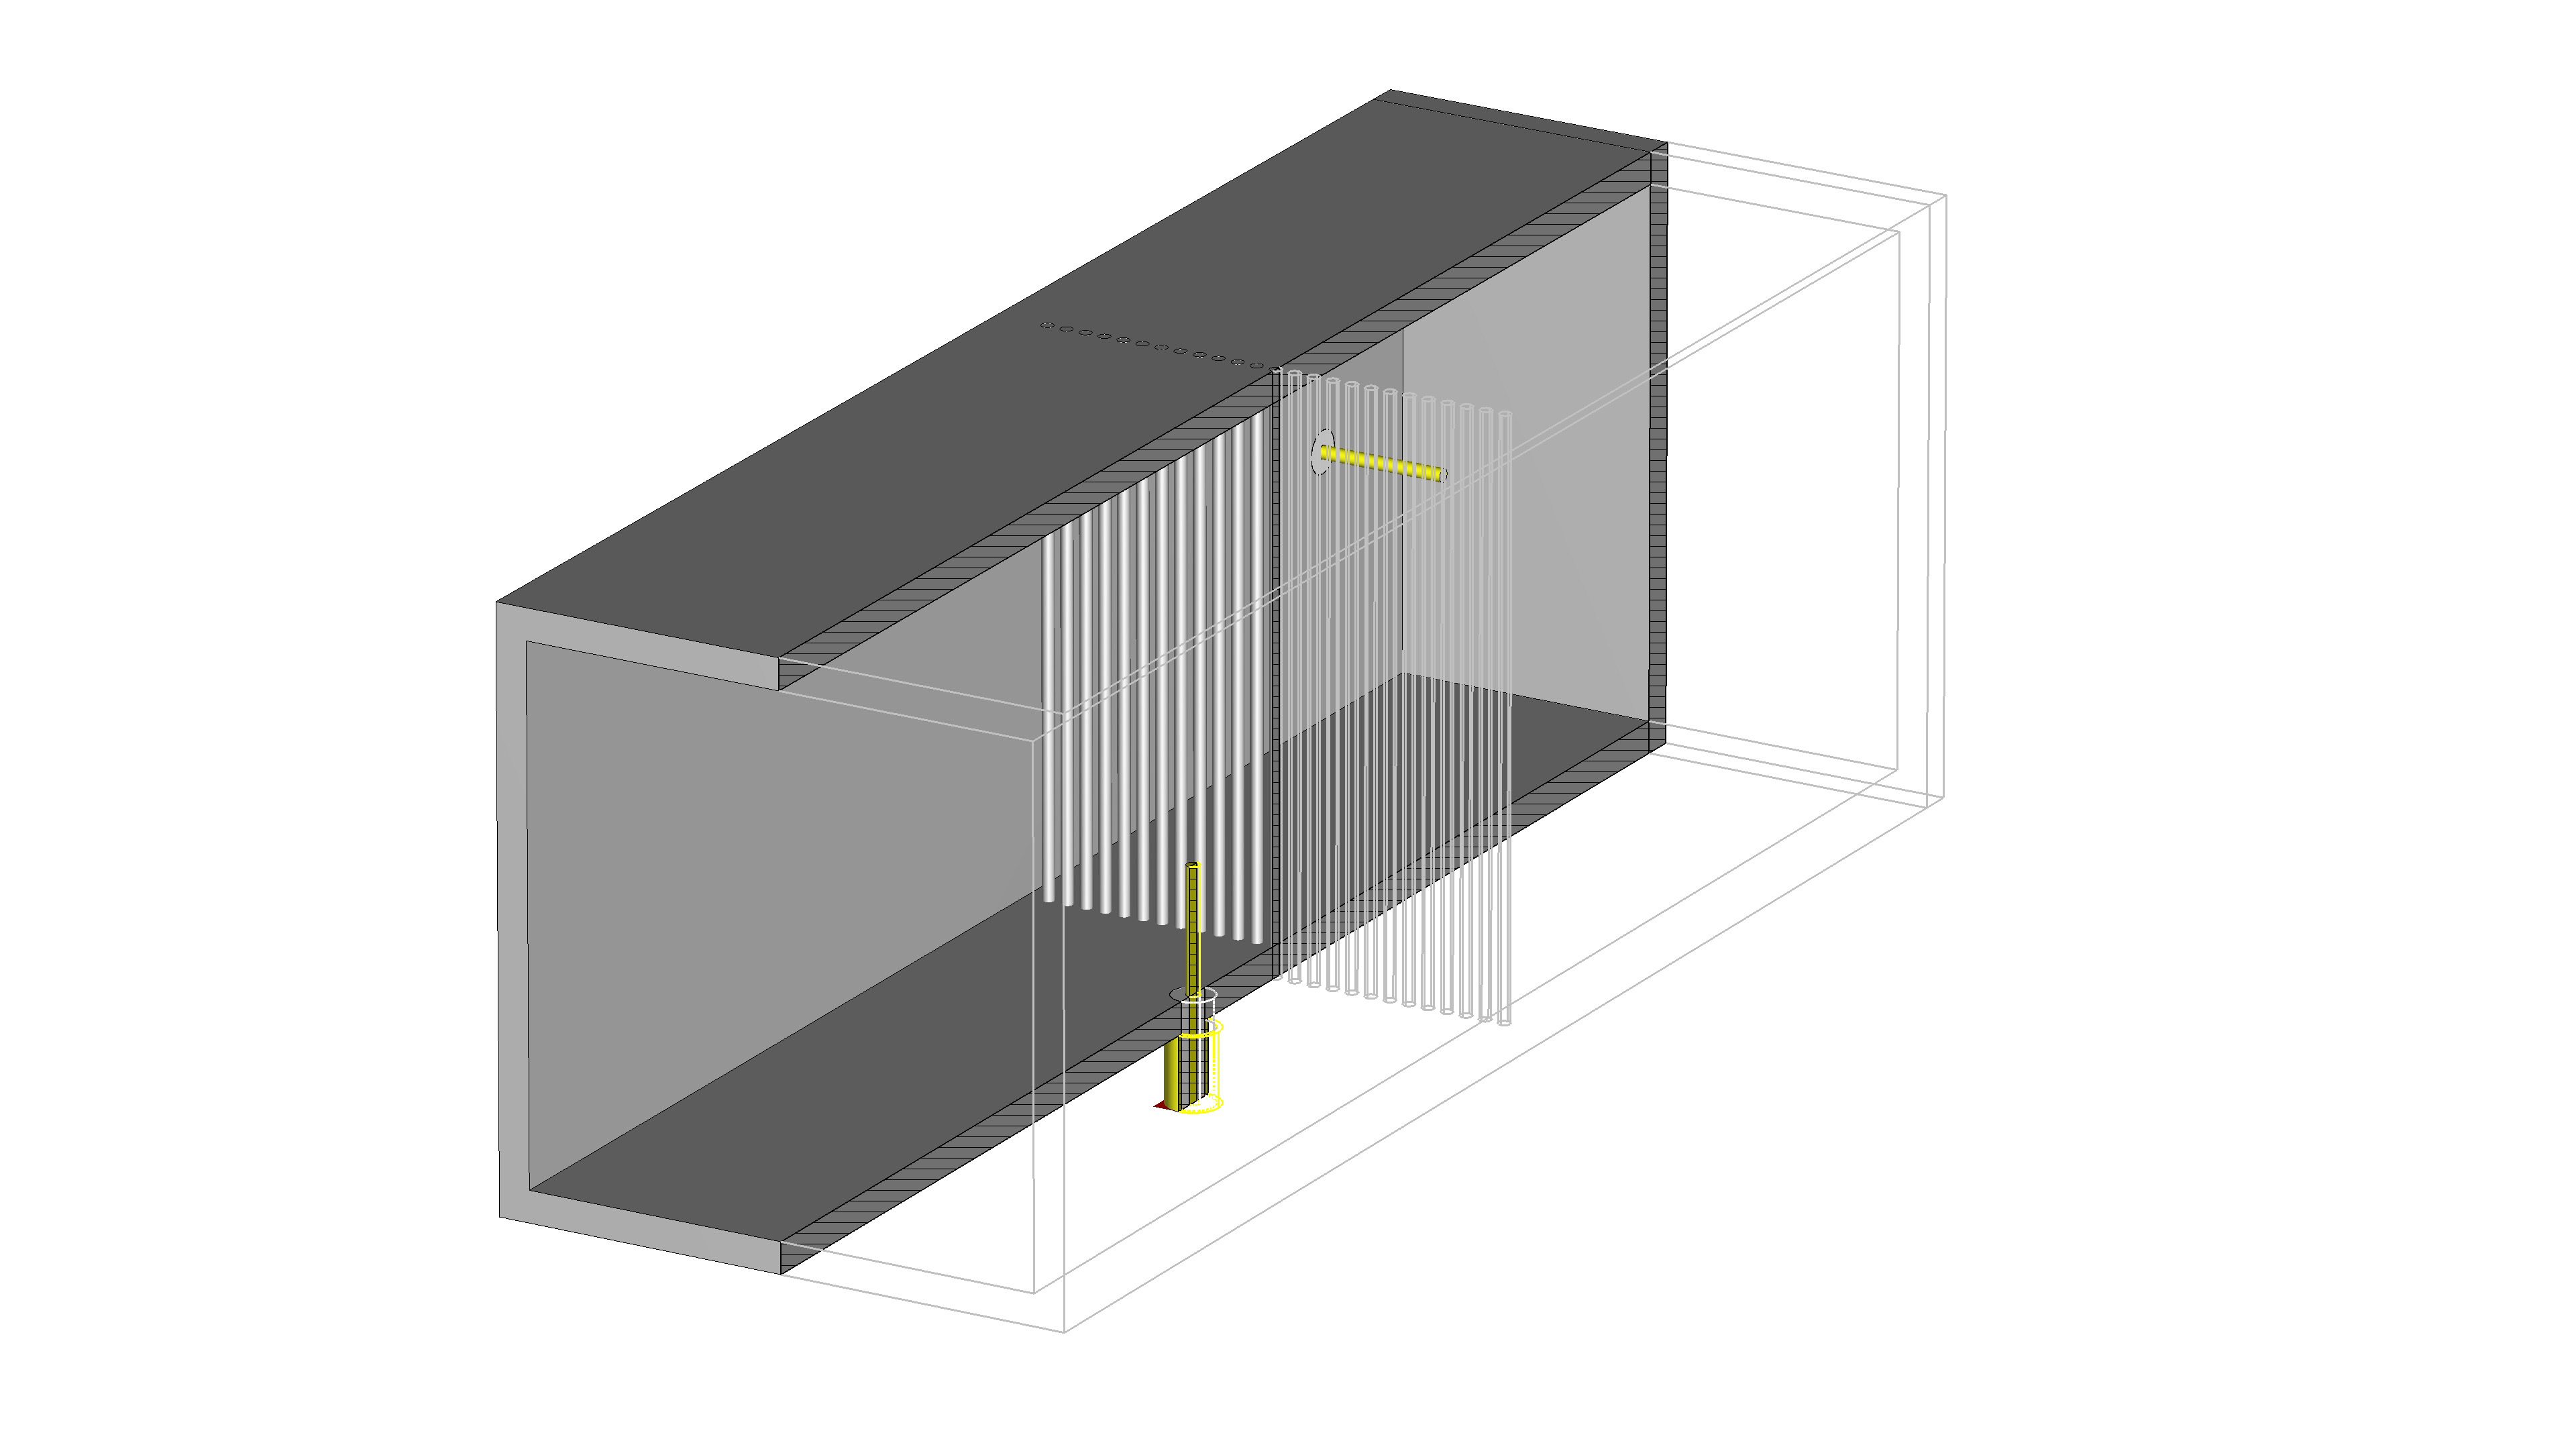
\includegraphics[width=.8\textwidth]{src/dual_feed_perspective.png}
    \caption{\label{fig:dual-feed-perspective}Final dual feed: model}
\end{figure}

\chapter{Antenna}
\label{chapter:antenna}
This chapter details the design of the third and final component of the system under consideration. As depicted in \cref{fig:polarizer-radiation}, the polarizer demonstrates the potential for generating waves with favourable far-field radiation characteristics. However, to facilitate a smooth transition between the waveguide and free space, the structure must be coupled with an antenna exhibiting moderate gain, approximately $\qty{15}{dBi}$. Furthermore, the antenna needs to support circular polarization. These requirements, particularly within the context of waveguide technology, suggest the utilization of a symmetrical antenna. While a pyramidal horn antenna with a square aperture could be inferred from the polarizer geometry, a conical horn antenna, adapted to the square polarizer outlet, is selected for this application due to its simpler fabrication process and robust support of circular polarization.

\section{Conical horn}
The radiation characteristics of conical horn antennas, including gain, aperture phase distributions, loss factors, and amplitude patterns, have been comprehensively re-examined in~\parencite{aboserwal-et-al:conical-horn-gain-and-amplitude-patterns} utilizing spherical and quadratic aperture phase distributions. Moreover, a novel methodology for accurate computation of far-field amplitude patterns, including those in the far side and back lobe regions, was developed therein. This methodology leverages geometrical optics and diffraction theory, incorporating the Method of Equivalent Currents, which utilizes magnetic source quantities as previously discussed in \cref{subsection:maxwells-equations}.

The theoretical work presented in~\parencite{aboserwal-et-al:conical-horn-gain-and-amplitude-patterns} and similar publications is anticipated to be integrated into the practical functionalities offered by Antenna Magus. This software facilitates the automatic synthesis of antenna designs, predicated on desired performance requirements, through neural networks. These networks are trained on an extensive database comprising existing antenna models and their corresponding performance data. Moreover, seamless integration with CST Studio Suite is supported, allowing for direct export of the synthesized antenna designs into the CST simulation environment for further analysis. An antenna model demonstrating this design approach, demanding the target gain of $\qty{15}{dBi}$ at the centre frequency of $\qty{5.2}{GHz}$, is illustrated in \cref{fig:conical-horn-magus-perspective}.

\begin{figure}[!ht]
    \centering
    \begin{subfigure}{.45\textwidth}
        \centering
        \includegraphics[width=\textwidth]{src/conical_horn_magus_perspective.png}
        \caption{\label{fig:conical-horn-magus-perspective}Antenna Magus}
    \end{subfigure}
    ~
    \begin{subfigure}{.45\textwidth}
        \centering
        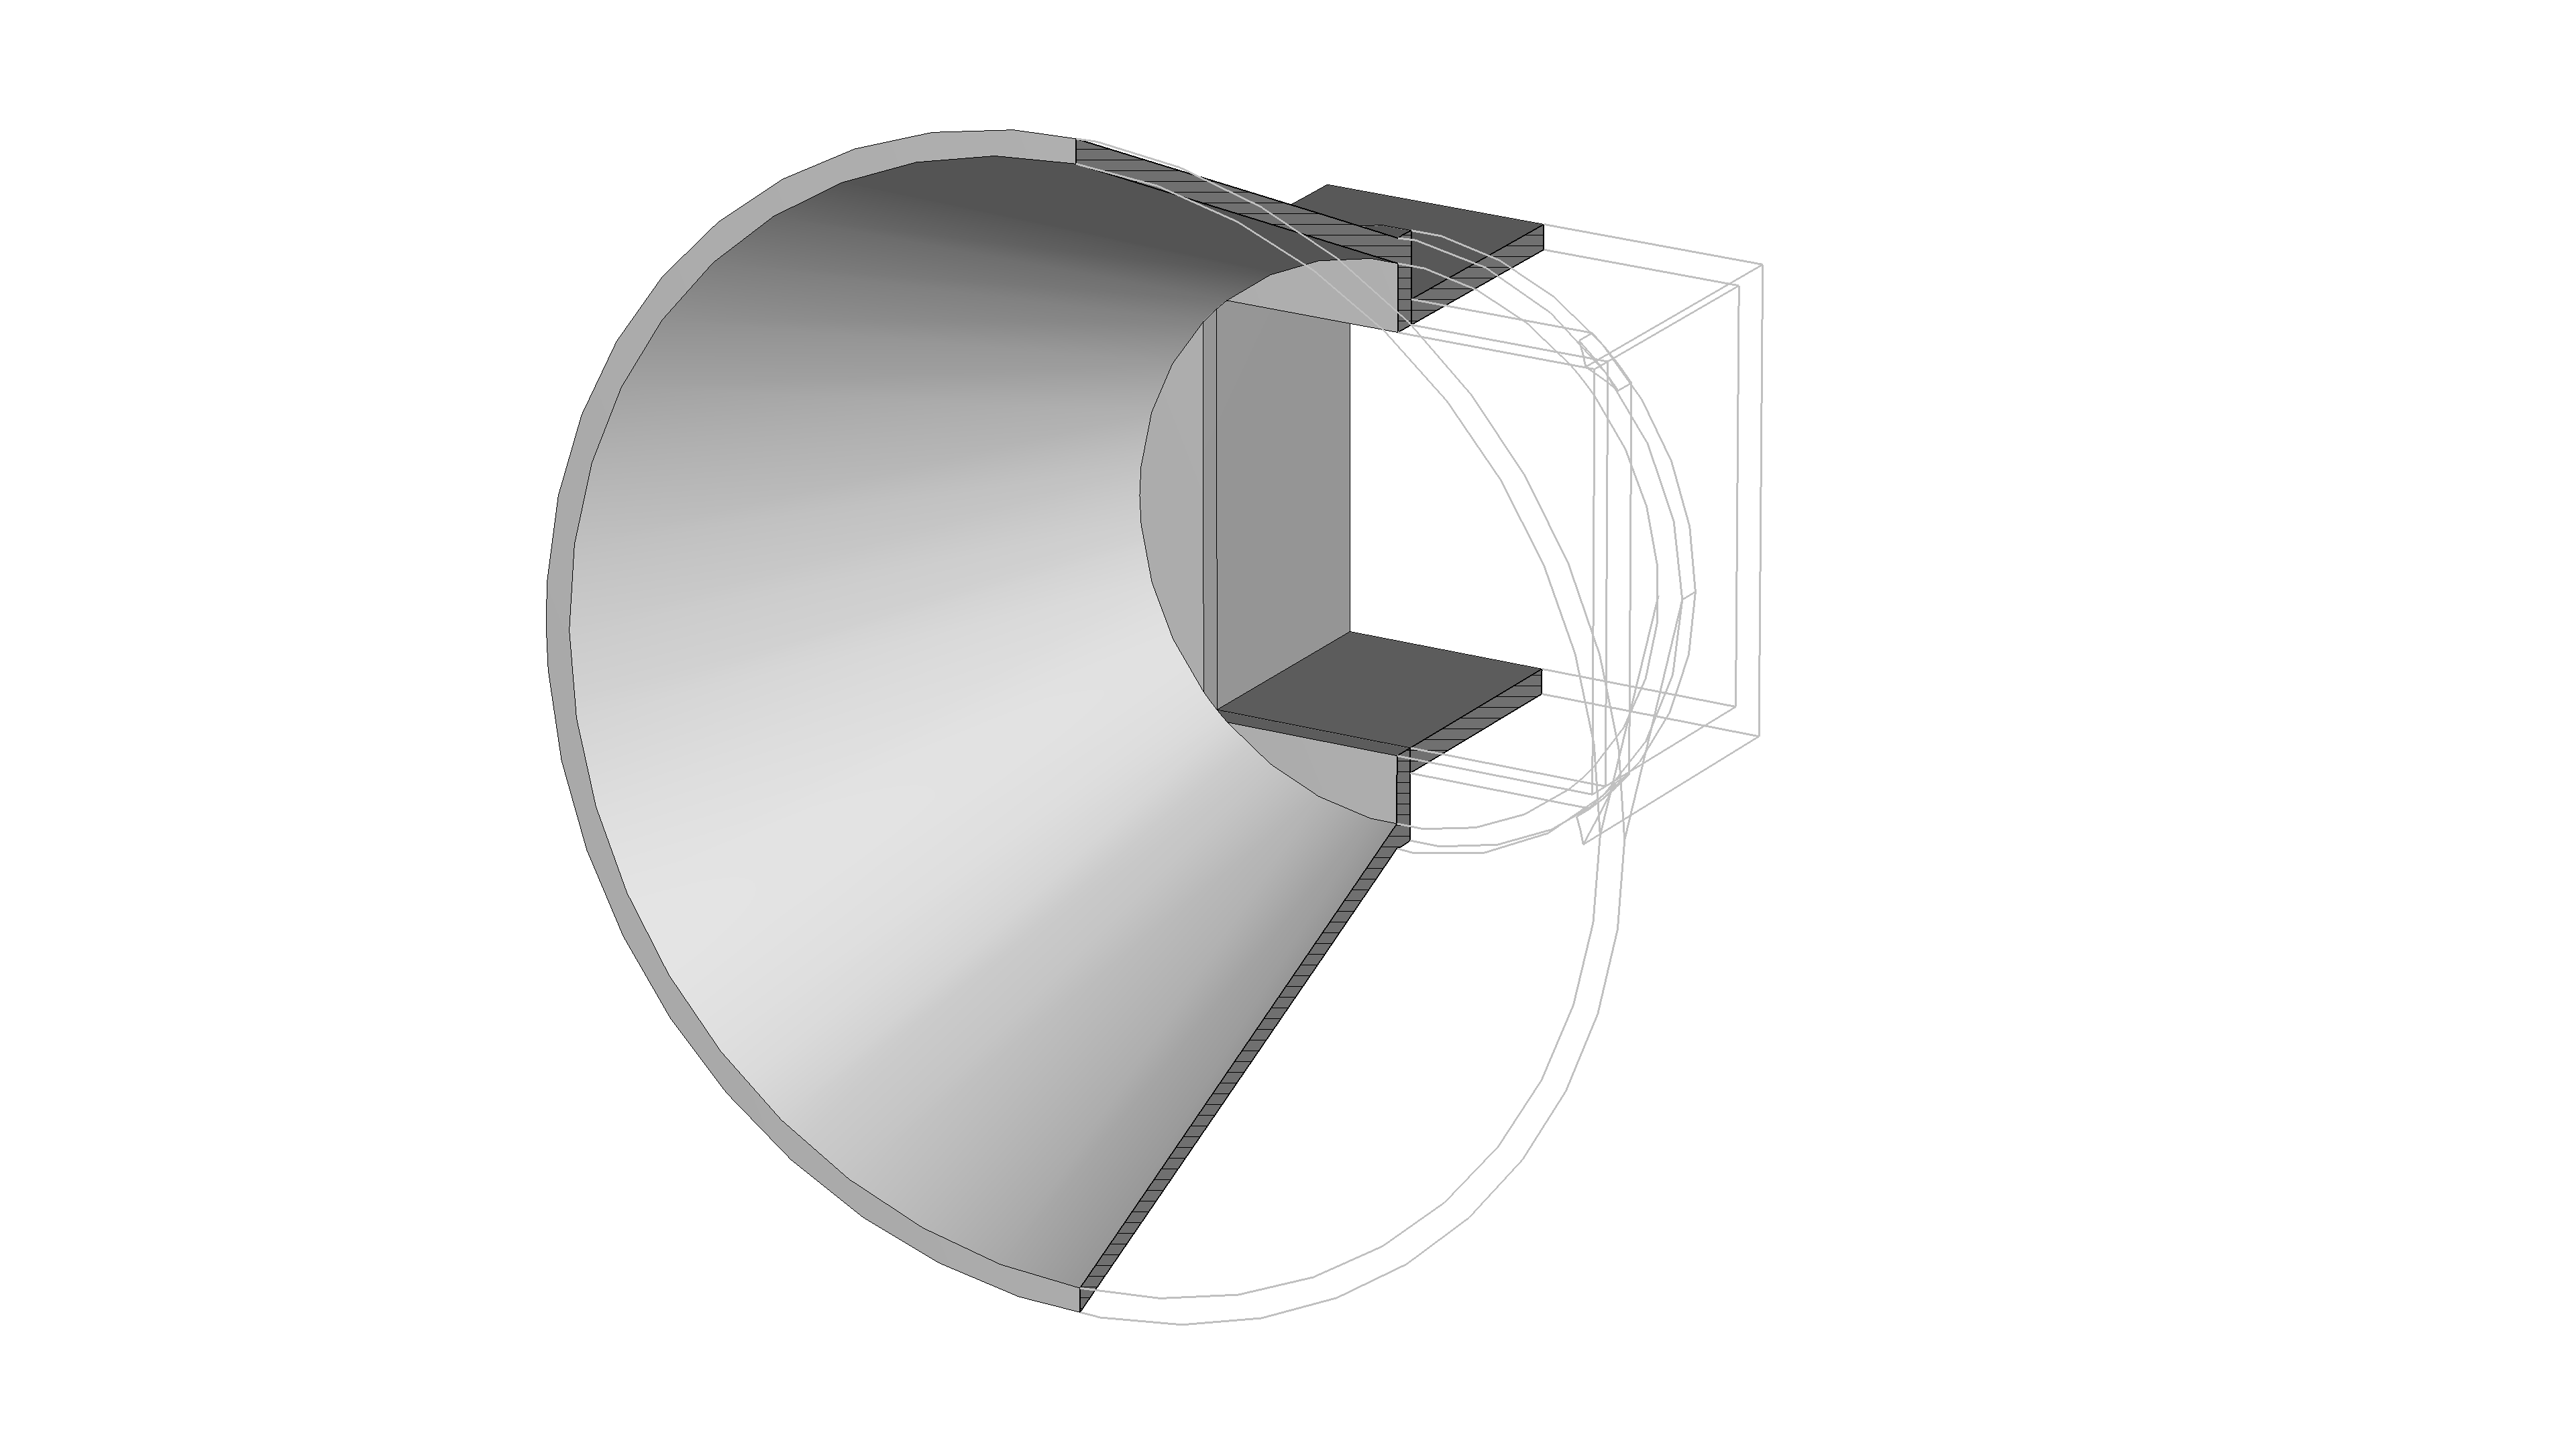
\includegraphics[width=\textwidth]{src/conical_horn_perspective.png}
        \caption{\label{fig:conical-horn-perspective}Finalized}
    \end{subfigure}
    \caption{\label{fig:conical-horn-models}Conical horn: models}
\end{figure}

The antenna depicted in \cref{fig:conical-horn-magus-perspective} provides a robust performance benchmark for subsequent adaptation into a rectangular waveguide configuration.  Maintaining the original horn dimensions while modifying the feed from a circular to a rectangular waveguide is hypothesized to yield comparable results, contingent upon a smooth rectangular-to-conical transition that minimizes reflections detrimental to horn performance. Parametric sweeps of the horn flare diameter, $D_f$, and flare length, $L_f$, indicate that the target gain can be realized through various combinations of these parameters. Notably, for each value of flare length, the relationship between gain and flare diameter exhibits a concave function characterized by a distinct local maximum.%
    \footnote{This behaviour is observed and examined in Figure 3 of~\parencite{aboserwal-et-al:conical-horn-gain-and-amplitude-patterns}.}
Consequently, the selection of optimal parameters necessitates a trade-off between achieving the desired gain with a sufficient margin and minimizing the overall antenna dimensions. Two promising configurations were identified:
\begin{enumerate}[label=(\alph*)]
    \item $D_f = \qty{120}{mm}$, $L_f = \qty{60}{mm}$, yielding a gain of $\qty{15}{dBi}$,
    \item $D_f = \qty{130}{mm}$, $L_f = \qty{70}{mm}$, yielding a gain of $\qty{15.5}{dBi}$.
\end{enumerate}
Ultimately, the latter configuration (b) was selected for the final design, prioritizing a larger gain margin despite the consequential increase in antenna dimensions. The finalized antenna design is depicted in \cref{fig:conical-horn-perspective}. Its performance is benchmarked against an idealized Antenna Magus design, which assumes perfect electric conductors and zero wall thickness. As illustrated in \cref{fig:conical-horn-performance-comparison}, the adaptation of the model to a square waveguide configuration resulted in some deviations in the figures of merit. Nevertheless, the overall performance remains highly satisfactory, adhering to the required performance thresholds.

\begin{figure}[!ht]
    \centering
    \includesvg[width=\textwidth]{src/conical_horns_comparison.svg}
    \caption{\label{fig:conical-horn-performance-comparison}Conical horn: performance}
\end{figure}

\chapter{Final structure}
\label{chapter:final-structure}
This concluding chapter details the finalization of the antenna design, transitioning from individual component designs presented in Chapter~\ref{chapter:polarizer}~through~\ref{chapter:antenna} to a fully integrated and manufacturable product. The process begins with an assessment of initial full-system simulation results and an analysis of identified discrepancies. Due to fabrication time constraints, a Minimum Viable Product (MVP) was developed, prioritizing core functionality. Subsequently, Design for Manufacturing (DFM) adjustments were incorporated into the structural design to ensure compatibility with CNC machining processes while preserving the desired electromagnetic performance. This involved modifications such as modularizing the antenna and adapting features for CNC drilling feasibility. The resulting DFM-compliant design was then fabricated and characterized by Universal Microwave Technology, Inc. The measured performance data is presented herein, along with a comparative analysis against the simulated results.

\section{Feed rework}
Preliminary simulations indicate that the performance of the final structure deviates significantly from expectations, particularly concerning the operation of the dual-feeding mechanism. This discrepancy is primarily reflected in the S-parameters, as illustrated in \cref{fig:grating-vs-mvp-sparameters}. While the performance of the feed incorporating a grating polarizer is acceptable in isolation, the figure also presents the S-parameters for a configuration with the grating entirely removed. This latter configuration represents the simplest implementation of a dual-feeding structure, previously discussed and dismissed in \cref{section:dual-feed} due to inherent high cross-talk between ports. However, as demonstrated in \cref{fig:grating-vs-mvp-sparameters}, the inclusion of a grating polarizer, despite exhibiting excellent individual performance, provides only negligible improvement in cross-talk mitigation. This minimal benefit comes at the expense of a substantial increase in manufacturing complexity, overall size, and consequently, the cost of the final product.

As previously addressed in \cref{section:dual-feed}, the manipulation of cross-talk levels can be achieved through an increase in grating density. Unfortunately, this approach concurrently results in a significant degradation of port reflections, with the values established in \cref{eq:dual-feed-optimum} representing the optimal compromise. Consequently, the integration of a grating polarizer fails to yield the anticipated performance improvements, attributable to an as-yet-unidentified mechanism. A comprehensive investigation of this underlying mechanism necessitates further research, which falls outside the current scope and timeline of this thesis, particularly considering the impending fabrication deadlines. Therefore, to expedite the development process, the MVP solution depicted in \cref{fig:final-perspective} is adopted. This design omits the grating polarizer and positions both ports within the same plane, ultimately proving to be an equally viable solution.

\begin{figure}[!ht]
    \centering
    \includesvg[width=\textwidth]{src/grating_vs_mvp_sparameters.svg}
    \caption{\label{fig:grating-vs-mvp-sparameters}Final structure: grating performance}
\end{figure}

% \begin{figure}[!ht]
%     \centering
%     \includesvg[width=\textwidth]{src/grating_vs_mvp_polarization.svg}
%     \caption{\label{fig:grating-vs-mvp-polarizations}Polarization gain}
% \end{figure}

\begin{figure}[!ht]
    \centering
    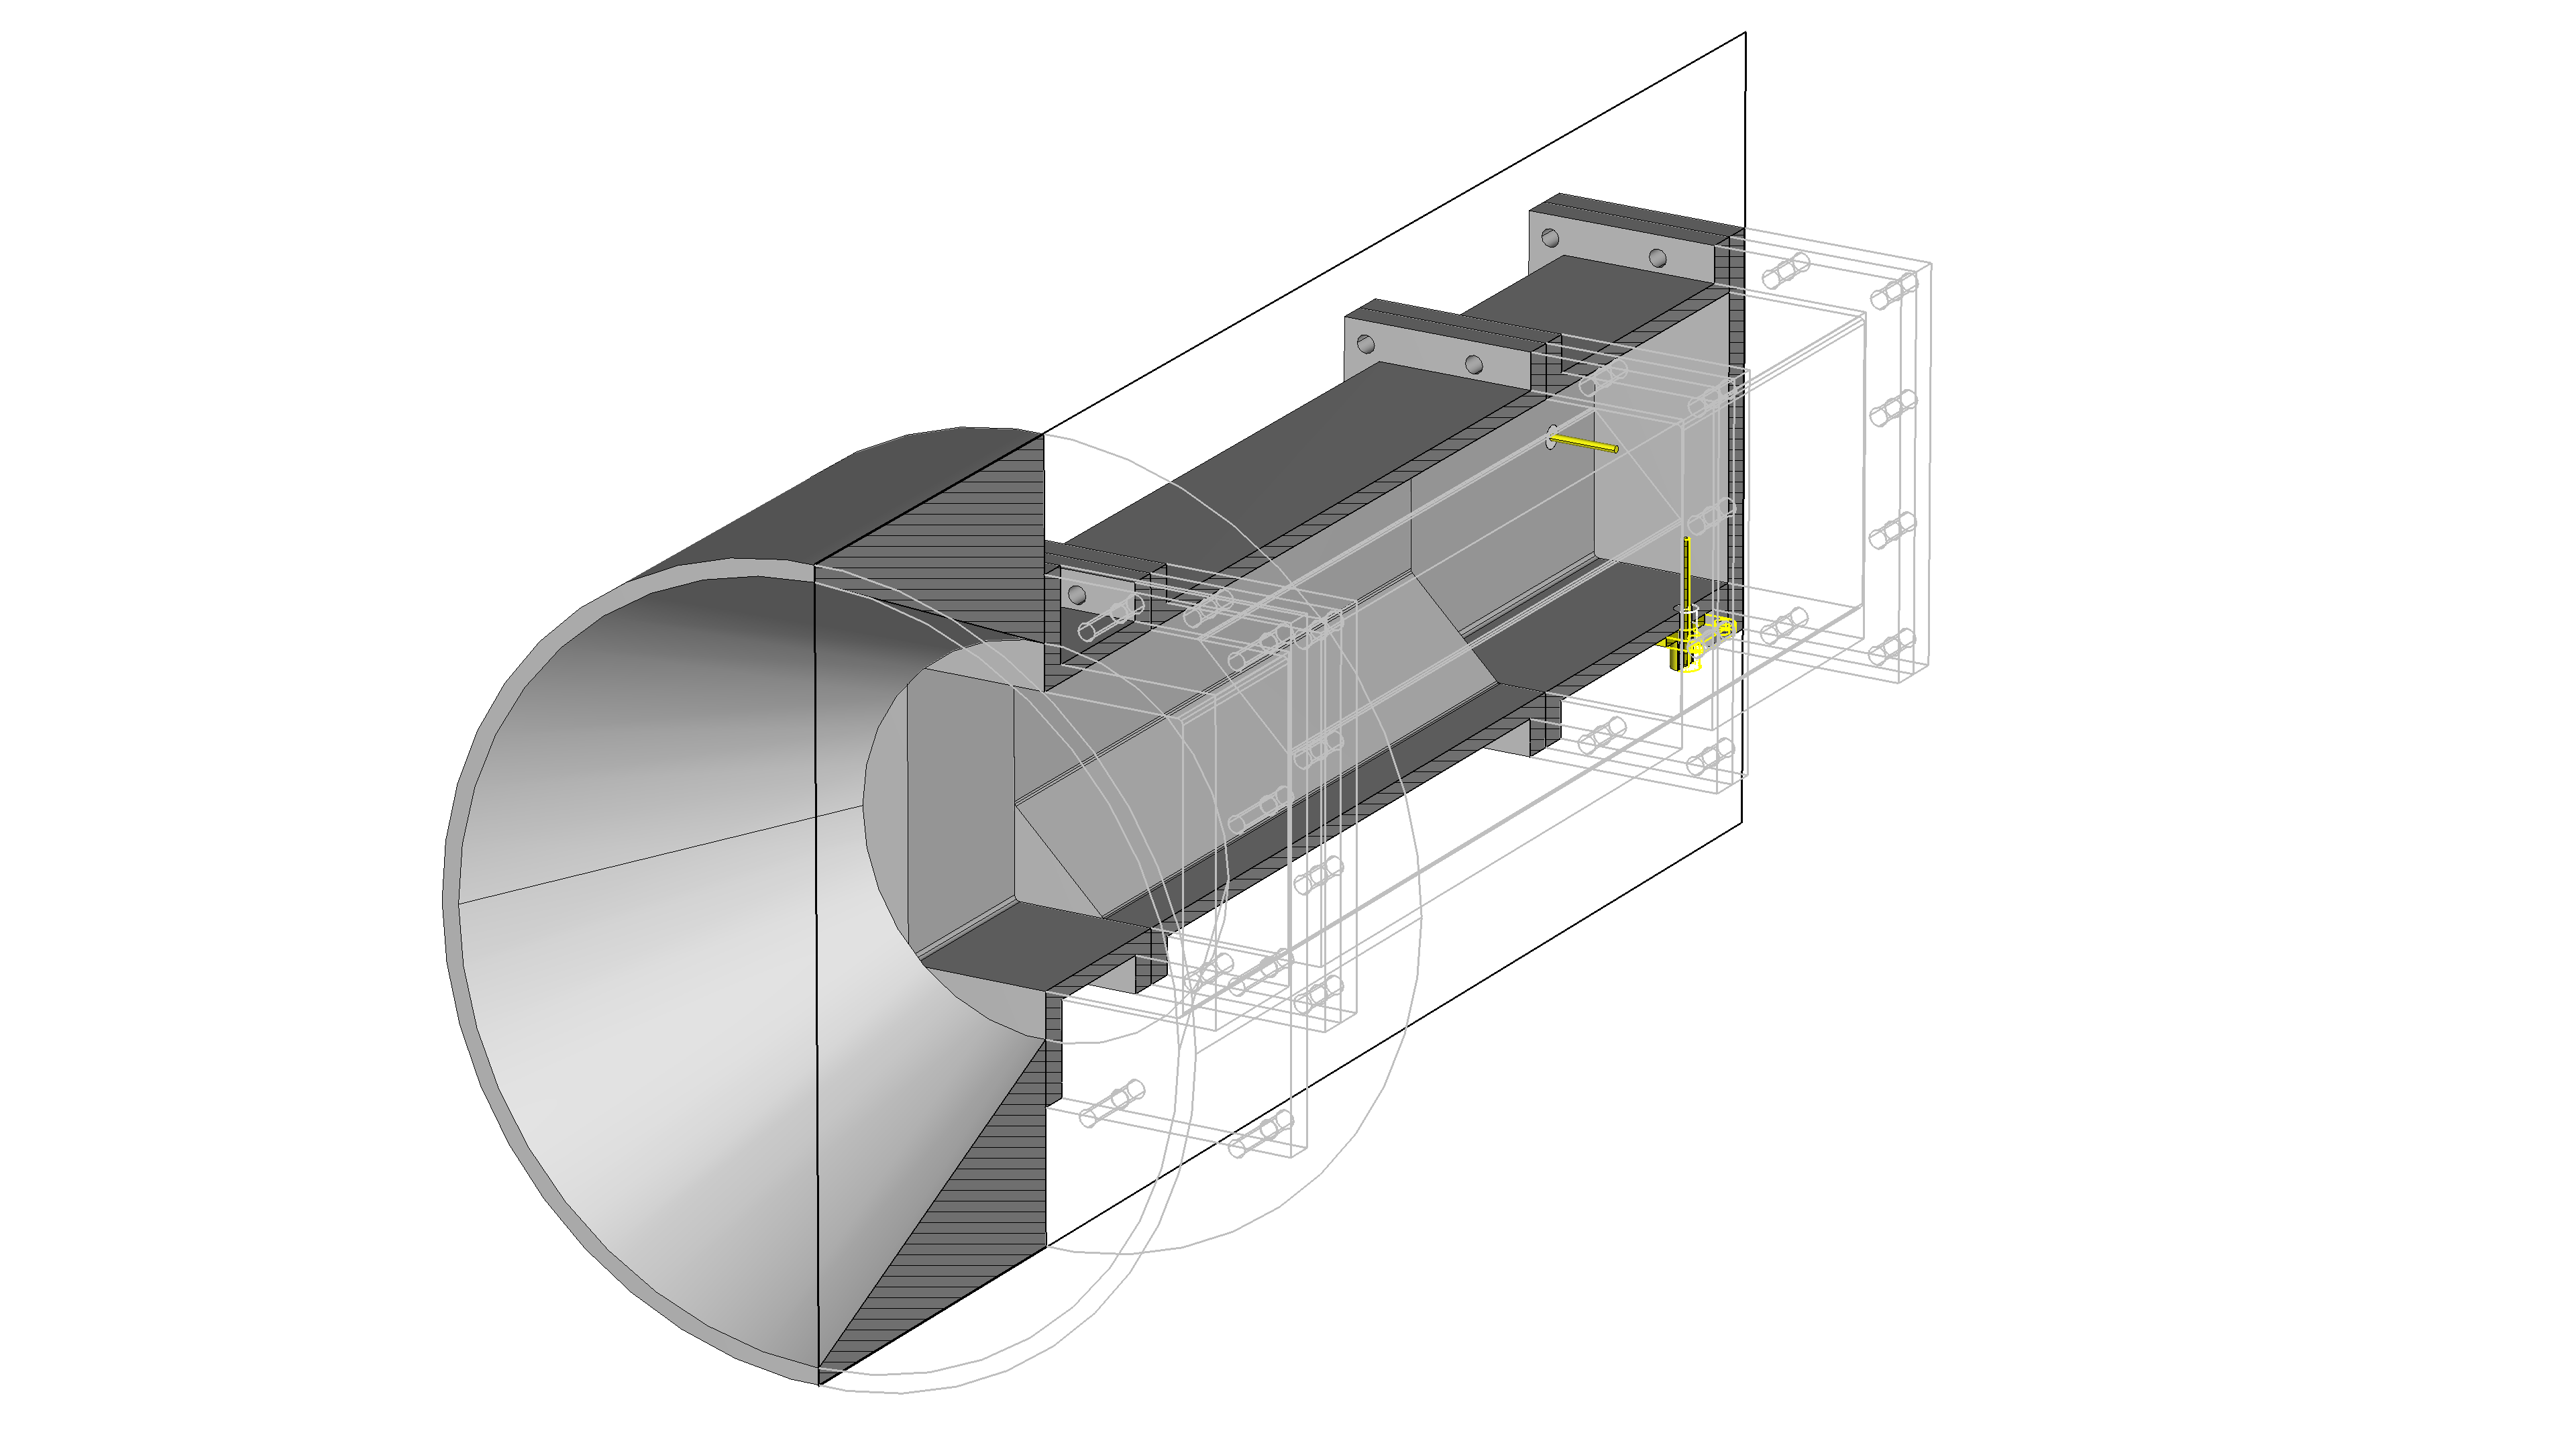
\includegraphics[width=.8\textwidth]{src/final_perspective.png}
    \caption{\label{fig:final-perspective}Final structure: MVP model}
\end{figure}

\section{Product finalization}
The structure illustrated in \cref{fig:final-perspective} represents the finalized model used for electromagnetic simulations, establishing a benchmark for subsequent comparison with measurement data. To ensure the utmost accuracy, these verification simulations employed exceptionally fine meshing settings and stringent convergence criteria based on energy dissipation. Concurrently, the final model underwent a design review with the principal engineer at Universal Microwave Technology, Inc. This consultation led to the implementation of final DFM modifications. These adjustments, aimed at ensuring compatibility with standard CNC machining processes, involved the modularization of the complete structure into five distinct components: the conical horn, square waveguide section, polarizer, dual-feed, and back-short. Each of these components was designed with standard waveguide flanges to facilitate assembly, and the antenna's geometry was further refined for efficient fabrication using drilling techniques. The resulting DFM-compliant model, depicted in \cref{fig:final-umt-perspective}, demonstrates that the internal dimensions remain unchanged, thereby preserving the critical electromagnetic performance characteristics of the original design.

\begin{figure}[!ht]
    \centering
    \includegraphics[width=.8\textwidth]{src/final_umt_perspective.png}
    \caption{\label{fig:final-umt-perspective}Final structure: DFM model}
\end{figure}

Universal Microwave Technology, Inc., is a leading company in the design, development and manufacturing of customized components, antennas and cables for the microwave and millimetre-wave frequency bands. Its state-of-the-art technology made it a perfect supplier with high confidence that the product would be fabricated with very little manufacturing tolerance. As expected and presented in \cref{fig:meas-vs-sim-sparameters,fig:meas-vs-sim-boresight-radiation}, the antenna performs in very good agreement with the precise simulations. The boresight gain shows slight positive deviation towards higher values which can be caused by a slight misalignment with the antenna axis, although the exact reason cannot be stated with certainty. These two figures are but a segment of all the measurement data which have been extracted in its entirety from the main matter of the thesis into \cref{appendix:measurement-results}. The appendix serves the purpose of uncluttering this discussing while preserving all measurement data taken, like a repository. The data presented in \cref{fig:meas-vs-sim-sparameters,fig:meas-vs-sim-boresight-radiation} are namely both taken from the second set of measurements as stated in the appendix.

\begin{figure}[!ht]
    \centering
    \includesvg[width=\textwidth]{src/meas_vs_sim_sparameters.svg}
    \caption{\label{fig:meas-vs-sim-sparameters}Measurement results: S-parameters}
\end{figure}

\begin{figure}[!ht]
    \centering
    \includesvg[width=\textwidth]{src/meas_vs_sim_boresight_radiation.svg}
    \caption{\label{fig:meas-vs-sim-boresight-radiation}Measurement results: polarization gains}
\end{figure}

%========== Conclusion ==========
\chapter*{Conclusion}
\label{chapter:conclusion}
\addcontentsline{toc}{chapter}{\nameref{chapter:conclusion}}

\lipsum[10-13]

\paragraph{Possible improvements:}
\begin{itemize}
    \item Polarizer: tapered transition into the prisms for lower reflections, as in~\parencite{bhardwaj-volakis:hexagonal-waveguide-based-circularly-polarized-horn-antennas-for-submmwave-terahertz-band}.
    \item Polarizer: perhaps various sections for wider operation bandwidth.
    \item Feed: disc-loaded, cylindrical, prismatic and other techniques of coaxial-to-waveguide transitions to improve bandwidth.
    \item Antenna: quad-ridge square pyramidal horn as a more robust option, especially with wider bandwidth requirements.
\end{itemize}

\appendix
%========== Appendix A: Constrained optimization ==========
\chapter{Constrained optimization}
\label{appendix:constrained-optimization}
In advanced optimization scenarios requiring algorithmic manipulation, such as geometric adjustments after new parameter values are set, the native optimization tool within CST Studio Suite is insufficient. While a range of settings is provided, the configuration is confined to optimization methods and algorithm-specific parameters. The remaining functionality is integrated within the operational framework of CST Studio Suite, thereby precluding the definition of proper constraints apart from specifying a bounding interval for each variable.

The CST Studio Suite installation, however, incorporates a collection of CST Python libraries, as documented in~\parencite{cst:python-libraries-documentation}. These libraries allow for external control of a CST Studio Suite instance and access to a subset of its features via a Python programming interface.  Fortunately, the available features provide the requisite components for the construction of an optimizer class, thus enabling the establishment of an interface between an external optimization algorithm and automated simulation processes.

\begin{lstlisting}[caption={Optimizer class initialization}, label={lst:init}, language=Python]
from cst.interface import DesignEnvironment
from cst.results import ProjectFile, ResultItem

class CSTOptimizer:

def __init__(
    self,
    project_path: str,
    optimization_config: dict[str, Any],
    vba_path: Optional[str] = None,
):
    self.project_path = project_path
    if vba_path:
        with open(vba_path, "r") as vba_file:
            self.check_geometry = vba_file.read()
    else:
        self.check_geometry = None
    self.cst = DesignEnvironment().connect_to_any_or_new()
    self.project = self.cst.open_project(self.project_path)
    self.result_module = ProjectFile(
        self.project_path, allow_interactive=True
    ).get_3d()
\end{lstlisting}

The code snippet in \cref{lst:init} illustrates a segment of the class initialization method. During initialization, the class receives the path to the target project, an optimization configuration in a dictionary data structure that allows for optimization method customization, results processing logic, objective functions and others, and an optional path to a VBA script. This script, if provided, is executed within CST Studio Suite using its built-in BASIC interpreter during each optimization step after new parameter values are set. Beyond this, the complete initialization method defines various runtime variables for progress tracking and unpacks the optimization configuration dictionary into individual attributes to enhance runtime efficiency. These latter components are not central to the described core functionality and are omitted in the snippet.

The primary motivation behind developing a custom optimizer lies in the ability to tailor the \emph{objective function}. This function is evaluated at each iteration of the optimization process, serving to quantify performance, termed the \emph{objective value}, for a given set of parameters suggested by the optimization algorithm. Within the context of simulation software, this typically involves updating the model with new parameter values, executing a simulation, and subsequently assessing the objective value. Constraints can thus be enforced by integrating a geometry check and potential adjustments after the model's structure is updated with the new parameter values. An implementation of this strategy within the optimizer class, with some minor details omitted for clarity, is presented in \cref{lst:objective_function}.

\begin{lstlisting}[caption={Objective function}, label={lst:objective_function}, language=Python]
def objective_function(self, x: np.ndarray) -> float:
    # Update parameters
    update_parameters = "Sub Main()\n"
    current_step = {}
    for name, value in zip(self.variable_names, x.round(5)):
        update_parameters += (
            f'StoreParameter("{name}", {value})\n'
        )
        current_step[name] = value
    update_parameters += (
        "RebuildOnParametricChange(True, False)\nEnd Sub\n"
    )
    self.project.schematic.execute_vba_code(
        update_parameters, timeout=None
    )
    # Execute geometry adjustment VBA script, if provided
    if self.check_geometry:
        self.project.schematic.execute_vba_code(
            self.check_geometry, timeout=None
        )
    # Run simulation
    try:
        self.project.modeler.run_solver()
        self.last_run_id += 1
    finally:
        self.project.save(include_results=True)
    # Evaluate objective value
    return self.evaluate_step(current_step)
\end{lstlisting}

For improved clarity and logical flow, the processing of simulation results is encapsulated within a dedicated method. This modular approach is beneficial due to the organization of CST Python libraries into multiple modules. As illustrated in \cref{lst:init}, the implementation utilizes the following two modules:
\begin{itemize}
    \item \texttt{cst.interface} provides classes that facilitate the interface for controlling CST Studio Suite.
    \item \texttt{cst.results} enables read-only access to one-dimensional results stored in CST project files.
\end{itemize}
As shown in \cref{lst:objective_function}, the main body of the objective function concludes with a completed simulation, followed by saving the project to ensure the accessibility of the project files to the result module. Subsequently, these results are processed and evaluated using the function detailed in \cref{lst:evaluate_step}. For brevity, the function evaluates the results using the \emph{Sum of Differences} norm. The full implementation allows for choosing the goal norm 
via the optimization configuration dictionary.

\begin{lstlisting}[caption={Optimization step evaluation}, label={lst:evaluate_step}, language=Python]
def evaluate_step(self, current_step: dict[str, Any]) -> float:
    # Get results
    results = [
        self.parse_results(
            self.result_module.get_result_item(
                treepath=goal["result"],
                run_id=self.last_run_id,
            ),
        )
        for goal in self.goals
    ]
    # Compute objective value
    objective_value = 0
    for result, goal in zip(results, self.goals):
        average_difference = sum(
            result - goal["target"]
        ) / len(result)
        objective_value += goal["weight"] * average_difference
    return objective_value
\end{lstlisting}

In addition to the core optimization routines, the optimizer class also incorporates ancillary methods, which are utilized in the presented listings. While these utilities play an essential role, they are not the primary focus of this discussion.  Among the utilities used in the listings are \texttt{get\_constraints} and \texttt{get\_options}, used in \cref{lst:minimize} and responsible for retrieving arguments relevant to the optimization method, and \texttt{parse\_results}, tasked with preparing raw data from CST.

The foundational elements established thus far -- simulation control, data retrieval, and performance evaluation -- facilitate the integration of established optimization methods. Such methods are commonly found in data-oriented programming languages, with a particularly robust and widely recognized implementation being available in the \emph{SciPy} library, an open-source scientific computing library for Python thoroughly documented in~\parencite{virtanen-et-al:scipy}.

\begin{lstlisting}[caption={Use of CSTOptimizer with SciPy}, label={lst:minimize}, language=Python]
from scipy.optimize import minimize

result = minimize(
    optimizer.objective_function,
    x0=np.array(optimizer.initial_values),
    method=optimizer.method,
    bounds=optimizer.bounds,
    constraints=optimizer.get_constraints(),
    options=optimizer.get_options(),
)
\end{lstlisting}

\Cref{lst:minimize} assembles the complete logic, integrating all previously described components to enable a full optimization process. While some supplementary logic concerning algorithm termination and the saving of optimal parameters is omitted here for brevity, all essential elements are present.

The VBA script executed within CST Studio Suite, as part of the process outlined in \cref{lst:objective_function}, which allows for geometry validation and potential adjustments following parametric modifications, represents the primary advantage of this approach. This entire side project originated as a solution to the problematic optimization behaviour described in \cref{subsection:dual-feed-optimization}. Therefore, the VBA script designed explicitly for adjusting the grating within a dual-feeding structure for a square waveguide is presented in \cref{lst:grating-adjustment}. This script serves both as a practical use case for the developed optimizer class and as a direct solution to the issue identified in the main body of this work.

\begin{lstlisting}[caption={Grating adjustment script}, label={lst:grating-adjustment}, language=VBScript]
waveguideSide = GetParameter("waveguideSide")
gratingGap = GetParameter("gratingGap")
wireDiameter = GetParameter("wireDiameter")
wireCount = GetParameter("wireCount")
Do While isGratingTooNarrow( _
        waveguideSide, gratingGap, _
        wireDiameter, wireCount)
    wireCount = wireCount + 2
Loop
Do While isIntersecting( _
        waveguideSide, gratingGap, _
        wireDiameter, wireCount)
    wireCount = wireCount - 2
    If wireCount < 1 Then
        Err.Raise vbObjectError + 100, _
            "Main", _
            "No feasible grating geometry found."
        Exit Sub
    End If
Loop
If wireCount <> GetParameter("wireCount") Then
    StoreParameter "wireCount", wireCount
    Call RebuildOnParametricChange(True, False)
End If
\end{lstlisting}

\Cref{lst:grating-adjustment} again represents a segment of a larger code base, omitting rudimentary steps like variable definitions and error handling for brevity. The script utilizes three custom functions. Two of these functions perform geometric validity checks related to two cases of invalid grating arrangements with varying gaps:
\begin{enumerate}[label=(\alph*)]
    \item A gap that is too narrow, resulting in a gap between the grating and waveguide walls.
    \item  A too wide gap, resulting in wires intersecting with the waveguide walls.
\end{enumerate}
These two cases are detected by the functions detailed in \cref{lst:is-grating-too-narrow} and \cref{lst:is-intersecting}, respectively. They are corrected in the main program loop by adding or removing grating wires as needed.

\begin{lstlisting}[caption={Check for a gap around the grating}, label={lst:is-grating-too-narrow}, language=VBScript]
Private Function isGratingTooNarrow( _
    waveguideSide As Double, _
    gratingGap As Double, _
    wireDiameter As Double, _
    wireCount As Integer _
) As Boolean
    Dim gapAroundGrating As Double
    gapAroundGrating = (waveguideSide - _
        wireCount * gratingGap - _
        wireDiameter) / 2
    If gapAroundGrating > gratingGap Then
        isGratingTooNarrow = True
    Else
        isGratingTooNarrow = False
    End If
End Function
\end{lstlisting}

\begin{lstlisting}[caption={Check for intersection with waveguide walls}, label={lst:is-intersecting}, language=VBScript]
Private Function isIntersecting( _
    waveguideSide As Double, _
    gratingGap As Double, _
    wireDiameter As Double, _
    wireCount As Integer _
) As Boolean
    Dim gratingEdge As Double
    gratingEdge = (wireCount - 1) / 2 * _
        gratingGap + wireDiameter / 2
    If gratingEdge > waveguideSide / 2 Then
        isIntersecting = True
    Else
        isIntersecting = False
    End If
End Function
\end{lstlisting}

%========== Appendix B: Measurement results ==========
\chapter{Measurement results}
\label{appendix:measurement-results}
This appendix presents a comprehensive collection of measurement data acquired from two separate measurement campaigns performed on the fabricated antenna prototype. The fabrication of the prototype and the subsequent measurements were expertly carried out by Universal Microwave Technology, Inc. Their contribution in bringing the design to a physical realization and meticulously characterizing its performance is gratefully acknowledged. These datasets are compiled here to ensure a clear and concise presentation within the main body of the thesis. While certain key results have been incorporated into the main discussion for direct comparison with simulated data, this appendix serves as a complete and detailed repository of all measured parameters.

Specifically, the data presented herein encompasses S-parameter measurements, providing insights into the antenna's impedance matching and power transmission characteristics. These measurements were performed using an Agilent Vector Network Analyzer (VNA). Additionally, the appendix includes the frequency responses of both boresight gain and boresight axial ratio, characterizing the antenna's performance across the operational bandwidth. These radiation properties, along with the radiation patterns, were measured in an in-house anechoic chamber using an open-ended waveguide as a sensing antenna. The radiation patterns are presented in the form of both elevation and azimuth cuts taken at frequencies of $\qty{5}{GHz}$, $\qty{5.3}{GHz}$, and $\qty{5.5}{GHz}$. This comprehensive dataset allows for a thorough and independent evaluation of the fabricated antenna's performance characteristics.

\newpage
\begin{figure}[!ht]
    \centering
    \includesvg[width=\textwidth]{src/meas1_sparameters.svg}
    \caption{\label{fig:meas1-sparameters}Measurement 1: S-parameters}
\end{figure}

\begin{figure}[!ht]
    \centering
    \includesvg[width=\textwidth]{src/meas1_boresight_radiation.svg}
    \caption{\label{fig:meas1-boresight-radiation}Measurement 1: polarization gains}
\end{figure}

\begin{figure}[!ht]
    \centering
    \includesvg[width=\textwidth]{src/meas1_elevation_radiation.svg}
    \caption{\label{fig:meas1-elevation-radiation}Measurement 1: elevation radiation pattern}
\end{figure}

\begin{figure}[!ht]
    \centering
    \includesvg[width=\textwidth]{src/meas1_azimuth_radiation.svg}
    \caption{\label{fig:meas1-azimuth-radiation}Measurement 1: azimuth radiation pattern}
\end{figure}

\begin{figure}[!ht]
    \centering
    \includesvg[width=\textwidth]{src/meas2_sparameters.svg}
    \caption{\label{fig:meas2-sparameters}Measurement 2: S-parameters}
\end{figure}

\begin{figure}[!ht]
    \centering
    \includesvg[width=\textwidth]{src/meas2_boresight_radiation.svg}
    \caption{\label{fig:meas2-boresight-radiation}Measurement 2: polarization gains}
\end{figure}

\begin{figure}[!ht]
    \centering
    \includesvg[width=\textwidth]{src/meas2_elevation_radiation.svg}
    \caption{\label{fig:meas2-elevation-radiation}Measurement 2: elevation radiation pattern}
\end{figure}

\begin{figure}[!ht]
    \centering
    \includesvg[width=\textwidth]{src/meas2_azimuth_radiation.svg}
    \caption{\label{fig:meas2-azimuth-radiation}Measurement 2: azimuth radiation pattern}
\end{figure}

%========== Nomenclature ==========
\printnomenclature

%========== Bibliography ==========
\printbibliography[heading=bibintoc]

% %========== Index ==========
\printindex

\end{document}
